 
%% bare_jrnl_compsoc.tex
%% V1.4b
%% 2015/08/26
%% by Michael Shell
%% See:
%% http://www.michaelshell.org/
%% for current contact information.
%%
%% This is a skeleton file demonstrating the use of IEEEtran.cls
%% (requires IEEEtran.cls version 1.8b or later) with an IEEE
%% Computer Society journal paper.
%%
%% Support sites:
%% http://www.michaelshell.org/tex/ieeetran/
%% http://www.ctan.org/pkg/ieeetran
%% and
%% http://www.ieee.org/

%%*************************************************************************
%% Legal Notice:
%% This code is offered as-is without any warranty either expressed or
%% implied; without even the implied warranty of MERCHANTABILITY or
%% FITNESS FOR A PARTICULAR PURPOSE! 
%% User assumes all risk.
%% In no event shall the IEEE or any contributor to this code be liable for
%% any damages or losses, including, but not limited to, incidental,
%% consequential, or any other damages, resulting from the use or misuse
%% of any information contained here.
%%
%% All comments are the opinions of their respective authors and are not
%% necessarily endorsed by the IEEE.
%%
%% This work is distributed under the LaTeX Project Public License (LPPL)
%% ( http://www.latex-project.org/ ) version 1.3, and may be freely used,
%% distributed and modified. A copy of the LPPL, version 1.3, is included
%% in the base LaTeX documentation of all distributions of LaTeX released
%% 2003/12/01 or later.
%% Retain all contribution notices and credits.
%% ** Modified files should be clearly indicated as such, including  **
%% ** renaming them and changing author support contact information. **
%%*************************************************************************


% *** Authors should verify (and, if needed, correct) their LaTeX system  ***
% *** with the testflow diagnostic prior to trusting their LaTeX platform ***
% *** with production work. The IEEE's font choices and paper sizes can   ***
% *** trigger bugs that do not appear when using other class files.       ***                          ***
% The testflow support page is at:
% http://www.michaelshell.org/tex/testflow/


\documentclass[10pt,journal,compsoc]{IEEEtran}
%
% If IEEEtran.cls has not been installed into the LaTeX system files,
% manually specify the path to it like:
% \documentclass[10pt,journal,compsoc]{../sty/IEEEtran}





% Some very useful LaTeX packages include:
% (uncomment the ones you want to load)


% *** MISC UTILITY PACKAGES ***
%
%\usepackage{ifpdf}
% Heiko Oberdiek's ifpdf.sty is very useful if you need conditional
% compilation based on whether the output is pdf or dvi.
% usage:
% \ifpdf
%   % pdf code
% \else
%   % dvi code
% \fi
% The latest version of ifpdf.sty can be obtained from:
% http://www.ctan.org/pkg/ifpdf
% Also, note that IEEEtran.cls V1.7 and later provides a builtin
% \ifCLASSINFOpdf conditional that works the same way.
% When switching from latex to pdflatex and vice-versa, the compiler may
% have to be run twice to clear warning/error messages.






% *** CITATION PACKAGES ***
%
\ifCLASSOPTIONcompsoc
  % IEEE Computer Society needs nocompress option
  % requires cite.sty v4.0 or later (November 2003)
  \usepackage[nocompress]{cite}
\else
  % normal IEEE
  \usepackage{cite}
\fi
% cite.sty was written by Donald Arseneau
% V1.6 and later of IEEEtran pre-defines the format of the cite.sty package
% \cite{} output to follow that of the IEEE. Loading the cite package will
% result in citation numbers being automatically sorted and properly
% "compressed/ranged". e.g., [1], [9], [2], [7], [5], [6] without using
% cite.sty will become [1], [2], [5]--[7], [9] using cite.sty. cite.sty's
% \cite will automatically add leading space, if needed. Use cite.sty's
% noadjust option (cite.sty V3.8 and later) if you want to turn this off
% such as if a citation ever needs to be enclosed in parenthesis.
% cite.sty is already installed on most LaTeX systems. Be sure and use
% version 5.0 (2009-03-20) and later if using hyperref.sty.
% The latest version can be obtained at:
% http://www.ctan.org/pkg/cite
% The documentation is contained in the cite.sty file itself.
%
% Note that some packages require special options to format as the Computer
% Society requires. In particular, Computer Society  papers do not use
% compressed citation ranges as is done in typical IEEE papers
% (e.g., [1]-[4]). Instead, they list every citation separately in order
% (e.g., [1], [2], [3], [4]). To get the latter we need to load the cite
% package with the nocompress option which is supported by cite.sty v4.0
% and later. Note also the use of a CLASSOPTION conditional provided by
% IEEEtran.cls V1.7 and later.

\usepackage{color}
\usepackage{booktabs} % For formal tables
\usepackage{url}
\usepackage{graphicx}
\usepackage{subfigure}
\usepackage{multirow}
\usepackage{xspace}
\usepackage{enumitem} % for itemize
\usepackage{hyperref}
\usepackage[normalem]{ulem}
\usepackage{soul}
\usepackage{balance}
\usepackage{comment}
\usepackage{amsmath}
\usepackage[dvipsnames]{xcolor}

\newcommand{\tool}{{\textsc{\small DiffTech}}\xspace}
\newcommand{\chen}[1]{\textcolor{red}{#1}}
\newcommand{\wang}[1]{\textcolor{blue}{#1}}
\newcommand{\revise}[1]{\textcolor{OliveGreen}{#1}}

% *** GRAPHICS RELATED PACKAGES ***
%
\ifCLASSINFOpdf
  % \usepackage[pdftex]{graphicx}
  % declare the path(s) where your graphic files are
  % \graphicspath{{../pdf/}{../jpeg/}}
  % and their extensions so you won't have to specify these with
  % every instance of \includegraphics
  % \DeclareGraphicsExtensions{.pdf,.jpeg,.png}
\else
  % or other class option (dvipsone, dvipdf, if not using dvips). graphicx
  % will default to the driver specified in the system graphics.cfg if no
  % driver is specified.
  % \usepackage[dvips]{graphicx}
  % declare the path(s) where your graphic files are
  % \graphicspath{{../eps/}}
  % and their extensions so you won't have to specify these with
  % every instance of \includegraphics
  % \DeclareGraphicsExtensions{.eps}
\fi
% graphicx was written by David Carlisle and Sebastian Rahtz. It is
% required if you want graphics, photos, etc. graphicx.sty is already
% installed on most LaTeX systems. The latest version and documentation
% can be obtained at: 
% http://www.ctan.org/pkg/graphicx
% Another good source of documentation is "Using Imported Graphics in
% LaTeX2e" by Keith Reckdahl which can be found at:
% http://www.ctan.org/pkg/epslatex
%
% latex, and pdflatex in dvi mode, support graphics in encapsulated
% postscript (.eps) format. pdflatex in pdf mode supports graphics
% in .pdf, .jpeg, .png and .mps (metapost) formats. Users should ensure
% that all non-photo figures use a vector format (.eps, .pdf, .mps) and
% not a bitmapped formats (.jpeg, .png). The IEEE frowns on bitmapped formats
% which can result in "jaggedy"/blurry rendering of lines and letters as
% well as large increases in file sizes.
%
% You can find documentation about the pdfTeX application at:
% http://www.tug.org/applications/pdftex






% *** MATH PACKAGES ***
%
%\usepackage{amsmath}
% A popular package from the American Mathematical Society that provides
% many useful and powerful commands for dealing with mathematics.
%
% Note that the amsmath package sets \interdisplaylinepenalty to 10000
% thus preventing page breaks from occurring within multiline equations. Use:
%\interdisplaylinepenalty=2500
% after loading amsmath to restore such page breaks as IEEEtran.cls normally
% does. amsmath.sty is already installed on most LaTeX systems. The latest
% version and documentation can be obtained at:
% http://www.ctan.org/pkg/amsmath





% *** SPECIALIZED LIST PACKAGES ***
%
%\usepackage{algorithmic}
% algorithmic.sty was written by Peter Williams and Rogerio Brito.
% This package provides an algorithmic environment fo describing algorithms.
% You can use the algorithmic environment in-text or within a figure
% environment to provide for a floating algorithm. Do NOT use the algorithm
% floating environment provided by algorithm.sty (by the same authors) or
% algorithm2e.sty (by Christophe Fiorio) as the IEEE does not use dedicated
% algorithm float types and packages that provide these will not provide
% correct IEEE style captions. The latest version and documentation of
% algorithmic.sty can be obtained at:
% http://www.ctan.org/pkg/algorithms
% Also of interest may be the (relatively newer and more customizable)
% algorithmicx.sty package by Szasz Janos:
% http://www.ctan.org/pkg/algorithmicx




% *** ALIGNMENT PACKAGES ***
%
%\usepackage{array}
% Frank Mittelbach's and David Carlisle's array.sty patches and improves
% the standard LaTeX2e array and tabular environments to provide better
% appearance and additional user controls. As the default LaTeX2e table
% generation code is lacking to the point of almost being broken with
% respect to the quality of the end results, all users are strongly
% advised to use an enhanced (at the very least that provided by array.sty)
% set of table tools. array.sty is already installed on most systems. The
% latest version and documentation can be obtained at:
% http://www.ctan.org/pkg/array


% IEEEtran contains the IEEEeqnarray family of commands that can be used to
% generate multiline equations as well as matrices, tables, etc., of high
% quality.




% *** SUBFIGURE PACKAGES ***
%\ifCLASSOPTIONcompsoc
%  \usepackage[caption=false,font=footnotesize,labelfont=sf,textfont=sf]{subfig}
%\else
%  \usepackage[caption=false,font=footnotesize]{subfig}
%\fi
% subfig.sty, written by Steven Douglas Cochran, is the modern replacement
% for subfigure.sty, the latter of which is no longer maintained and is
% incompatible with some LaTeX packages including fixltx2e. However,
% subfig.sty requires and automatically loads Axel Sommerfeldt's caption.sty
% which will override IEEEtran.cls' handling of captions and this will result
% in non-IEEE style figure/table captions. To prevent this problem, be sure
% and invoke subfig.sty's "caption=false" package option (available since
% subfig.sty version 1.3, 2005/06/28) as this is will preserve IEEEtran.cls
% handling of captions.
% Note that the Computer Society format requires a sans serif font rather
% than the serif font used in traditional IEEE formatting and thus the need
% to invoke different subfig.sty package options depending on whether
% compsoc mode has been enabled.
%
% The latest version and documentation of subfig.sty can be obtained at:
% http://www.ctan.org/pkg/subfig




% *** FLOAT PACKAGES ***
%
%\usepackage{fixltx2e}
% fixltx2e, the successor to the earlier fix2col.sty, was written by
% Frank Mittelbach and David Carlisle. This package corrects a few problems
% in the LaTeX2e kernel, the most notable of which is that in current
% LaTeX2e releases, the ordering of single and double column floats is not
% guaranteed to be preserved. Thus, an unpatched LaTeX2e can allow a
% single column figure to be placed prior to an earlier double column
% figure.
% Be aware that LaTeX2e kernels dated 2015 and later have fixltx2e.sty's
% corrections already built into the system in which case a warning will
% be issued if an attempt is made to load fixltx2e.sty as it is no longer
% needed.
% The latest version and documentation can be found at:
% http://www.ctan.org/pkg/fixltx2e


%\usepackage{stfloats}
% stfloats.sty was written by Sigitas Tolusis. This package gives LaTeX2e
% the ability to do double column floats at the bottom of the page as well
% as the top. (e.g., "\begin{figure*}[!b]" is not normally possible in
% LaTeX2e). It also provides a command:
%\fnbelowfloat
% to enable the placement of footnotes below bottom floats (the standard
% LaTeX2e kernel puts them above bottom floats). This is an invasive package
% which rewrites many portions of the LaTeX2e float routines. It may not work
% with other packages that modify the LaTeX2e float routines. The latest
% version and documentation can be obtained at:
% http://www.ctan.org/pkg/stfloats
% Do not use the stfloats baselinefloat ability as the IEEE does not allow
% \baselineskip to stretch. Authors submitting work to the IEEE should note
% that the IEEE rarely uses double column equations and that authors should try
% to avoid such use. Do not be tempted to use the cuted.sty or midfloat.sty
% packages (also by Sigitas Tolusis) as the IEEE does not format its papers in
% such ways.
% Do not attempt to use stfloats with fixltx2e as they are incompatible.
% Instead, use Morten Hogholm'a dblfloatfix which combines the features
% of both fixltx2e and stfloats:
%
% \usepackage{dblfloatfix}
% The latest version can be found at:
% http://www.ctan.org/pkg/dblfloatfix




%\ifCLASSOPTIONcaptionsoff
%  \usepackage[nomarkers]{endfloat}
% \let\MYoriglatexcaption\caption
% \renewcommand{\caption}[2][\relax]{\MYoriglatexcaption[#2]{#2}}
%\fi
% endfloat.sty was written by James Darrell McCauley, Jeff Goldberg and 
% Axel Sommerfeldt. This package may be useful when used in conjunction with 
% IEEEtran.cls'  captionsoff option. Some IEEE journals/societies require that
% submissions have lists of figures/tables at the end of the paper and that
% figures/tables without any captions are placed on a page by themselves at
% the end of the document. If needed, the draftcls IEEEtran class option or
% \CLASSINPUTbaselinestretch interface can be used to increase the line
% spacing as well. Be sure and use the nomarkers option of endfloat to
% prevent endfloat from "marking" where the figures would have been placed
% in the text. The two hack lines of code above are a slight modification of
% that suggested by in the endfloat docs (section 8.4.1) to ensure that
% the full captions always appear in the list of figures/tables - even if
% the user used the short optional argument of \caption[]{}.
% IEEE papers do not typically make use of \caption[]'s optional argument,
% so this should not be an issue. A similar trick can be used to disable
% captions of packages such as subfig.sty that lack options to turn off
% the subcaptions:
% For subfig.sty:
% \let\MYorigsubfloat\subfloat
% \renewcommand{\subfloat}[2][\relax]{\MYorigsubfloat[]{#2}}
% However, the above trick will not work if both optional arguments of
% the \subfloat command are used. Furthermore, there needs to be a
% description of each subfigure *somewhere* and endfloat does not add
% subfigure captions to its list of figures. Thus, the best approach is to
% avoid the use of subfigure captions (many IEEE journals avoid them anyway)
% and instead reference/explain all the subfigures within the main caption.
% The latest version of endfloat.sty and its documentation can obtained at:
% http://www.ctan.org/pkg/endfloat
%
% The IEEEtran \ifCLASSOPTIONcaptionsoff conditional can also be used
% later in the document, say, to conditionally put the References on a 
% page by themselves.




% *** PDF, URL AND HYPERLINK PACKAGES ***
%
%\usepackage{url}
% url.sty was written by Donald Arseneau. It provides better support for
% handling and breaking URLs. url.sty is already installed on most LaTeX
% systems. The latest version and documentation can be obtained at:
% http://www.ctan.org/pkg/url
% Basically, \url{my_url_here}.





% *** Do not adjust lengths that control margins, column widths, etc. ***
% *** Do not use packages that alter fonts (such as pslatex).         ***
% There should be no need to do such things with IEEEtran.cls V1.6 and later.
% (Unless specifically asked to do so by the journal or conference you plan
% to submit to, of course. )


% correct bad hyphenation here
\hyphenation{op-tical net-works semi-conduc-tor}


\begin{document}
%
% paper title
% Titles are generally capitalized except for words such as a, an, and, as,
% at, but, by, for, in, nor, of, on, or, the, to and up, which are usually
% not capitalized unless they are the first or last word of the title.
% Linebreaks \\ can be used within to get better formatting as desired.
% Do not put math or special symbols in the title.
%\title{Tell Them Apart: Distilling Technology Differences from Crowd-Scale Comparison Discussions}
\title{DiffTech: Differencing Similar Technologies from Crowd-Scale Comparison Discussions}
%
%
% author names and IEEE memberships
% note positions of commas and nonbreaking spaces ( ~ ) LaTeX will not break
% a structure at a ~ so this keeps an author's name from being broken across
% two lines.
% use \thanks{} to gain access to the first footnote area
% a separate \thanks must be used for each paragraph as LaTeX2e's \thanks
% was not built to handle multiple paragraphs
%
%
%\IEEEcompsocitemizethanks is a special \thanks that produces the bulleted
% lists the Computer Society journals use for "first footnote" author
% affiliations. Use \IEEEcompsocthanksitem which works much like \item
% for each affiliation group. When not in compsoc mode,
% \IEEEcompsocitemizethanks becomes like \thanks and
% \IEEEcompsocthanksitem becomes a line break with idention. This
% facilitates dual compilation, although admittedly the differences in the
% desired content of \author between the different types of papers makes a
% one-size-fits-all approach a daunting prospect. For instance, compsoc 
% journal papers have the author affiliations above the "Manuscript
% received ..."  text while in non-compsoc journals this is reversed. Sigh.

\author{Michael~Shell,~\IEEEmembership{Member,~IEEE,}
        John~Doe,~\IEEEmembership{Fellow,~OSA,}
        and~Jane~Doe,~\IEEEmembership{Life~Fellow,~IEEE}% <-this % stops a space
\IEEEcompsocitemizethanks{\IEEEcompsocthanksitem M. Shell was with the Department
of Electrical and Computer Engineering, Georgia Institute of Technology, Atlanta,
GA, 30332.\protect\\
% note need leading \protect in front of \\ to get a newline within \thanks as
% \\ is fragile and will error, could use \hfil\break instead.
E-mail: see http://www.michaelshell.org/contact.html
\IEEEcompsocthanksitem J. Doe and J. Doe are with Anonymous University.}% <-this % stops an unwanted space
\thanks{Manuscript received April 19, 2005; revised August 26, 2015.}}

% note the % following the last \IEEEmembership and also \thanks - 
% these prevent an unwanted space from occurring between the last author name
% and the end of the author line. i.e., if you had this:
% 
% \author{....lastname \thanks{...} \thanks{...} }
%                     ^------------^------------^----Do not want these spaces!
%
% a space would be appended to the last name and could cause every name on that
% line to be shifted left slightly. This is one of those "LaTeX things". For
% instance, "\textbf{A} \textbf{B}" will typeset as "A B" not "AB". To get
% "AB" then you have to do: "\textbf{A}\textbf{B}"
% \thanks is no different in this regard, so shield the last } of each \thanks
% that ends a line with a % and do not let a space in before the next \thanks.
% Spaces after \IEEEmembership other than the last one are OK (and needed) as
% you are supposed to have spaces between the names. For what it is worth,
% this is a minor point as most people would not even notice if the said evil
% space somehow managed to creep in.



% The paper headers
\markboth{Journal of \LaTeX\ Class Files,~Vol.~14, No.~8, August~2015}%
{Shell \MakeLowercase{\textit{et al.}}: Bare Demo of IEEEtran.cls for Computer Society Journals}
% The only time the second header will appear is for the odd numbered pages
% after the title page when using the twoside option.
% 
% *** Note that you probably will NOT want to include the author's ***
% *** name in the headers of peer review papers.                   ***
% You can use \ifCLASSOPTIONpeerreview for conditional compilation here if
% you desire.



% The publisher's ID mark at the bottom of the page is less important with
% Computer Society journal papers as those publications place the marks
% outside of the main text columns and, therefore, unlike regular IEEE
% journals, the available text space is not reduced by their presence.
% If you want to put a publisher's ID mark on the page you can do it like
% this:
%\IEEEpubid{0000--0000/00\$00.00~\copyright~2015 IEEE}
% or like this to get the Computer Society new two part style.
%\IEEEpubid{\makebox[\columnwidth]{\hfill 0000--0000/00/\$00.00~\copyright~2015 IEEE}%
%\hspace{\columnsep}\makebox[\columnwidth]{Published by the IEEE Computer Society\hfill}}
% Remember, if you use this you must call \IEEEpubidadjcol in the second
% column for its text to clear the IEEEpubid mark (Computer Society jorunal
% papers don't need this extra clearance.)



% use for special paper notices
%\IEEEspecialpapernotice{(Invited Paper)}



% for Computer Society papers, we must declare the abstract and index terms
% PRIOR to the title within the \IEEEtitleabstractindextext IEEEtran
% command as these need to go into the title area created by \maketitle.
% As a general rule, do not put math, special symbols or citations
% in the abstract or keywords.
\IEEEtitleabstractindextext{%
\begin{abstract}
	
	Developers can use different technologies for many software development tasks in their work.
	However, when faced with several technologies with comparable functionalities, it is not easy for developers to select the most appropriate one, as comparisons among technologies are time-consuming by trial and error.
	Instead, developers can resort to expert articles, read official documents or ask questions in Q\&A sites for technology comparison, but it is opportunistic to get a comprehensive comparison as online information is often fragmented or contradictory.
	To overcome these limitations, we propose the \textit{diffTech} system that exploits the crowdsourced discussions from Stack Overflow, and assists technology comparison with an informative summary of different comparison aspects.
	We first build a large database of comparable technologies in software engineering by mining tags in Stack Overflow, and then locate comparative sentences about comparable technologies with natural language processing methods.
	We further mine prominent comparison aspects by clustering similar comparative sentences and representing each cluster with its keywords.
	The evaluation demonstrates both the accuracy and usefulness of our model and we implement our approach into a practical website for public use.
	
\end{abstract}

% Note that keywords are not normally used for peerreview papers.
\begin{IEEEkeywords}
differencing similar technology, Stack Overflow, NLP
\end{IEEEkeywords}}


% make the title area
\maketitle


% To allow for easy dual compilation without having to reenter the
% abstract/keywords data, the \IEEEtitleabstractindextext text will
% not be used in maketitle, but will appear (i.e., to be "transported")
% here as \IEEEdisplaynontitleabstractindextext when the compsoc 
% or transmag modes are not selected <OR> if conference mode is selected 
% - because all conference papers position the abstract like regular
% papers do.
\IEEEdisplaynontitleabstractindextext
% \IEEEdisplaynontitleabstractindextext has no effect when using
% compsoc or transmag under a non-conference mode.



% For peer review papers, you can put extra information on the cover
% page as needed:
% \ifCLASSOPTIONpeerreview
% \begin{center} \bfseries EDICS Category: 3-BBND \end{center}
% \fi
%
% For peerreview papers, this IEEEtran command inserts a page break and
% creates the second title. It will be ignored for other modes.
\IEEEpeerreviewmaketitle


\IEEEraisesectionheading{\section{Introduction}\label{sec:introduction}}

%BACKGROUND
A diverse set of technologies (e.g, algorithms, programming languages, platforms, libraries/frameworks, concepts for software engineering)~\cite{chen2016explore, chen2016techland} is available for use by developers and that set continues growing.
By adopting suitable technologies, it will significantly accelerate the software development process and also enhance the software quality.
But when developers are looking for proper technologies for their tasks, they are likely to find several comparable candidates.
For example, they will find \textit{bubble sort} and \textit{quick sort} algorithms for sorting, \textit{nltk} and \textit{opennlp} libraries for NLP, \textit{Eclipse} and \textit{Intellij} for developing Java applications.
%\textcolor{red}{CCY: Will revise the examples after obtaining all results.}

%POTENTIAL methods
Faced with so many candidates, developers are expected to have a good understanding of different technologies in order to make a proper choice for their work.
However, even for experienced developers, it can be difficult to keep pace with the rapid evolution of technologies.
Developers can try each of the candidates in their work for the comparison.
%, or read documentations, tutorials, examples of each candidate technology.
%\textcolor{blue}{??XINGZC: How about official documentation of a technology? They will describe what the technology is good for. There are two papers ``Patterns of knowledge in API reference documentation'' and ``A field study of API learning resources''. The first one shows that quality and environment knowledge is almost never present and explains that this knowledge remains tacit in the mind of API developers. The second one shows that developers need this type of knowledge to perform their work. At least for API comparison, we can say official documentation is not enough}.
But such trial-and-error assessment is time-consuming and labor extensive.
Instead, we find that the perceptions of developers about comparable technologies and the choices they make about which technology to use are very likely to be influenced by how other developers \textit{see} and \textit{evaluate} the technologies.
So developers often turn to the two information sources on the Web~\cite{bao2017extracting} to learn more about comparable technologies.

First, they read experts' articles about technology comparison like \href{https://dzone.com/articles/why-idea-better-eclipse}{\textit{``Intellij vs. Eclipse: Why IDEA is Better''}}.
Second, developers can seek answers on Q\&A websites such as Stack Overflow or Quora (e.g., \href{https://stackoverflow.com/questions/47011991/apache-open-nlp-vs-nltk}{\textit{``Apache OpenNLP vs NLTK''}}).
These expert articles and community answers are indexable by search engines, thus enabling developers to find answers to their technology comparison inquiries.

\begin{figure}
	\centering
	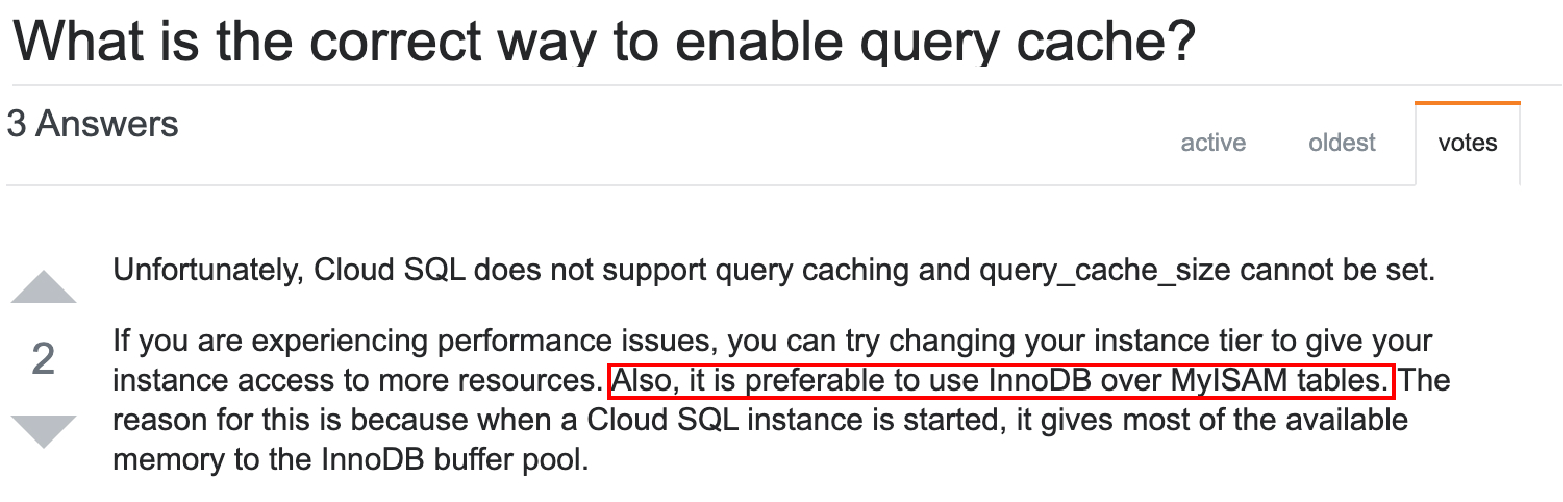
\includegraphics[width=0.47\textwidth]{figures/fig1.pdf}
	
	\vspace{-5mm}
	\caption{A comparative sentence in a question (\#30654296) that is not explicitly for technology comparison.}
	\label{fig:example}
	\vspace{-3mm}
\end{figure}

%LIMITATION of the potential methods
%\textcolor{red}{CCY: I remove two limitations due to their vulnurability, please have a look. In addition, our work cannot also solve the ``diverse opinions'' .}
However, there are two limitations with expert articles and community answers.
%[leftmargin=*]
\begin{itemize}[leftmargin=*]
	%\item \textit{Out of date:} The technology itself is in a constant state of change, while expert articles and community answers, once posted, are rarely updated, leaving the knowledge in them out of date.\textcolor{red}{CCY: Please find some examples to illustrate the first point.}
	
	\item \textit{Fragmented view:} An expert article or community answer usually focuses on a specific aspect of some comparable technologies, and developers have to aggregate the fragmented information into a complete comparison in different aspects.
	For example, to compare \textit{mysql} and \textit{postgresql}, one article~\cite{web:mysql1} contrasts their speed, while another~\cite{web:mysql2} compares their reliability.
	Only after reading both articles, developers can have a relatively comprehensive overview of these two comparable technologies.
	
	%\item \textit{Only intentional comparisons:} Expert articles and community answers cover some technology comparisons that developers intentionally make, but there are much more ``unintended'' knowledge hidden in the Q\&A discussions that do not intentionally discuss or compare technologies. 
	%\item \textit{Personal opinions:} Experts write their own opinions about the similar technologies they use. But their statement of the pros and cons may not be reliable, as the conclusion may be obtained by misusing the technologies or from just personal feelings without hard evidence. 
	%\textcolor{red}{Note that many of these comparative sentences are not present in posts that intentionally discuss or compare two technologies. Instead, hey are widely present when users answer other types of questions. 
	%Fig.\ref{fig:example} shows such as example: the answer ``accidentally'' compares the security of \textit{POST} and \textit{GET}, while the question ``How secure is a HTTP post?'' does not explicit ask for this comparison.
	
	\item \textit{Diverse opinions:} One expert article or community answer is based on the author's knowledge and experience. %??XINGZC: This point could bite back. We fundamentally analyze and summarize community answers. If community answers is questionable because they are opinion-based, then how can our summary be good? Do we have some measurements to tell who are more trustable?}.
	%\textcolor{red}{CCY: We mitigate that problem for three reasons: 1)we only use answers larger than 0 score which means all sentence has been checked by at least one user; 2)we provide multiple comparative sentences for each pair of similar technology, and user can check the crowd opinion rather than one.}
	However, the knowledge and experience of developers vary greatly.
	For example, one developer may prefer \textit{Eclipse} over \textit{Intellij} because \textit{Eclipse} fits his project setting better.
	But that setting may not be extensible to other developers.
	At the same time, some developers may prefer \textit{Intellij} over \textit{Eclipse} for other reasons.
	Such contradictory preferences among different opinions may confuse developers. 
	
\end{itemize}
%Expert articles and community answers have three limitations.

%In this work, we propose a model to aggregate such separated implicit users' opinions as a whole to explicitly compare similar technologies.

%\textcolor{blue}{I formulate the research problem as all the four limitations create difficulties in aggregating information manually. Our approach provides an automated solution to aggregate information.}
The above two limitations create a high barrier for developers to effectively gather useful information about technology differences on the Web in order to tell apart comparable technologies.
Although developers may manually aggregate relevant information by searching and reading many web pages, that would be very opportunistic and time consuming.
To overcome the above limitations, we present the \textit{diffTech} system that automatically distills and aggregates fragmented and trustworthy technology comparison information from the crowd-scale Q\&A discussions in Stack Overflow, and assists technology comparison with an informative summary of different aspects of comparison information.
%Note that the technology differences our system aggregates may be originally scattered in many posts that do not intentionally compare technologies.

Our system is motivated by the fact that a wide range of technologies have been discussed by millions of users in Stack Overflow~\cite{chen2016towards}, and users often express their preferences toward a technology and compare one technology with the others in the discussions.
Apart from posts explicitly about the comparison of some technologies, many comparative sentences \textbf{hide} in posts that are implicitly about technology comparison.
Fig.\ref{fig:example} shows such an example: the answer ``accidentally'' compares \textit{Innodb} and \textit{Myisam}, while the question ``What is the correct way to enable query cache?'' does not explicit ask for this comparison.
Inspired by such phenomenon, we then propose our system to mine and aggregate the comparative sentences in Stack Overflow discussions.

As shown in Fig.~\ref{fig:overview}, we consider Stack Overflow tags as a collection of technology terms and first find comparable technologies by analyzing tag embeddings and categories.
\revise{Our system then mines comparative opinions from Q\&A discussions by analyzing sentence patterns, calculating word mover distance~\cite{kusner2015word} and community detection~\cite{girvan2002community} to cluster comparative sentences into different aspects by which users compare the two technologies for user inspection. 
Finally, we fine-tune the BERT~\cite{devlin2018bert} model to summarize overall sentiment from all the comparative sentences for each comparable technology pairs.}
%\textcolor{red}{I think that we hide out-of-date problems.}
%\textcolor{blue}{Our system analyzes the metadata of the posts from which technology comparison information is extracted, such as post time, post score, post owner's reputation score, to distill likely up-to-date and trustworthy information about technology differences ??XINGZC: from your early comment, I think we analyze post score. How about post owner's reputation? May also be a good indicator of information quality. Furthermore, if we mention out of date as a limitation, we better have some ways to deal with it, for example, by considering the post time, more recent, more up to date. Do not need to do any analysis. Just present some metadata information like post time, user reputation score, post score when showing the comparative sentences is enough.}.
%\textcolor{red}{We then locate the comparative sentences that ...}


As there is no ground truth for technology comparison, we manually validate the performance of each step of our approach. 
The experiment results confirm the accuracy of comparable technology identification (90.7\%), and distilling comparative sentences (89.1\%) from Q\&A discussions.
% recall (\textcolor{red}{??\%})
\revise{By manually building the ground truth, we show that our clustering method (word mover distance and community detection) for comparative sentences significantly outperforms other baselines. 
Regarding the accuracy of overall sentiment summarization, our model also boost \chen{??\%} improvement compared with the baselines.
In addition, we also demonstrate the generality of our approach by successfully extracting comparative opinions of comparable technologies in other domain-specific datasets.}


\begin{comment}
Our first task is to \textcolor{red}{find similar technologies in software engineering domain ??XINGZC: should we reference to our similartech and say this paper extends it to broader technologies?}.
\textcolor{blue}{CCY: ASE is double-blind, we cannot say that is our previous work.}
In Stack Overflow, each question is attached with several tags and each tag is a keyword or a software-specific term which shows what topics this questions resolves.
So we take the tags in Stack Overflow as the representatives of technologies.
We adopt word embedding to tag sentences to obtain tag vector which capture the semantic of tags.
In the vector space, the more closed tag vectors, the more similar are the tags.
\end{comment}

%For example, a user may state that a library is better in speed or easier to learn than the other library in one post, which provides detailed opinions on these technologies.
%As a result, these comparative sentences can be very helpful in summarizing technology comparisons.

%\textcolor{blue}{With comparative sentences that compare two technologies directly ??XINGZC: we should explain that such comparative sentences are not just present in posts that intentionally discuss and compare two technologies. Instead, they are widely present when users answer other types of questions. Is this the case? We may need to collect some data to prove this and also show that those non-intentional comparative sentences cover more pairs of technologies and broader points about these technologies than those intentional comparison posts. Otherwise, people may challenge us ``why not just return the accepted or the most voted answers to those intentional comparison posts?''}, \textcolor{red}{CCY: Good point and I added it below in red.} 


%This paper proposes a method to identify and summarize comparative opinions from Stack Overflow automatically.
%A \textit{comparative opinion} is defined as a comparative sentence which compares the one technology with another, while expressing the user's sentiment on a chosen topic such as memory usage, usability, and performance.

\revise{This paper is an extended version of our earlier study~\cite{huang2018tell}, the extension makes the following additional contributions:
\begin{itemize}
	\item Apart from the existing single-sentence patterns, we also take the context and coreference into the consideration for discovering more comparative sentences about similar technologies.
	%Our model can not only spot the similar technologies, but also their differences.
	\item To give developers an clear overview, we develop a classifier for identifying the sentiment towards each technology, and aggregate the crowd opinions in total.
	\item Based on the extracted comparative opinions, we implement a practical website\footnote{\url{https://difftech.herokuapp.com/}} for developers looking for technology comparison knowledge. The analysis of site visiting logs demonstrate the usefulness of our tool. 
	\item  We not only update previous experiments by including new data and new baselines, but also add more detailed analysis of experiments results. We also demonstrate the generality of our method in other domain-specific datasets.
\end{itemize}
}

\begin{figure}
	\centering
	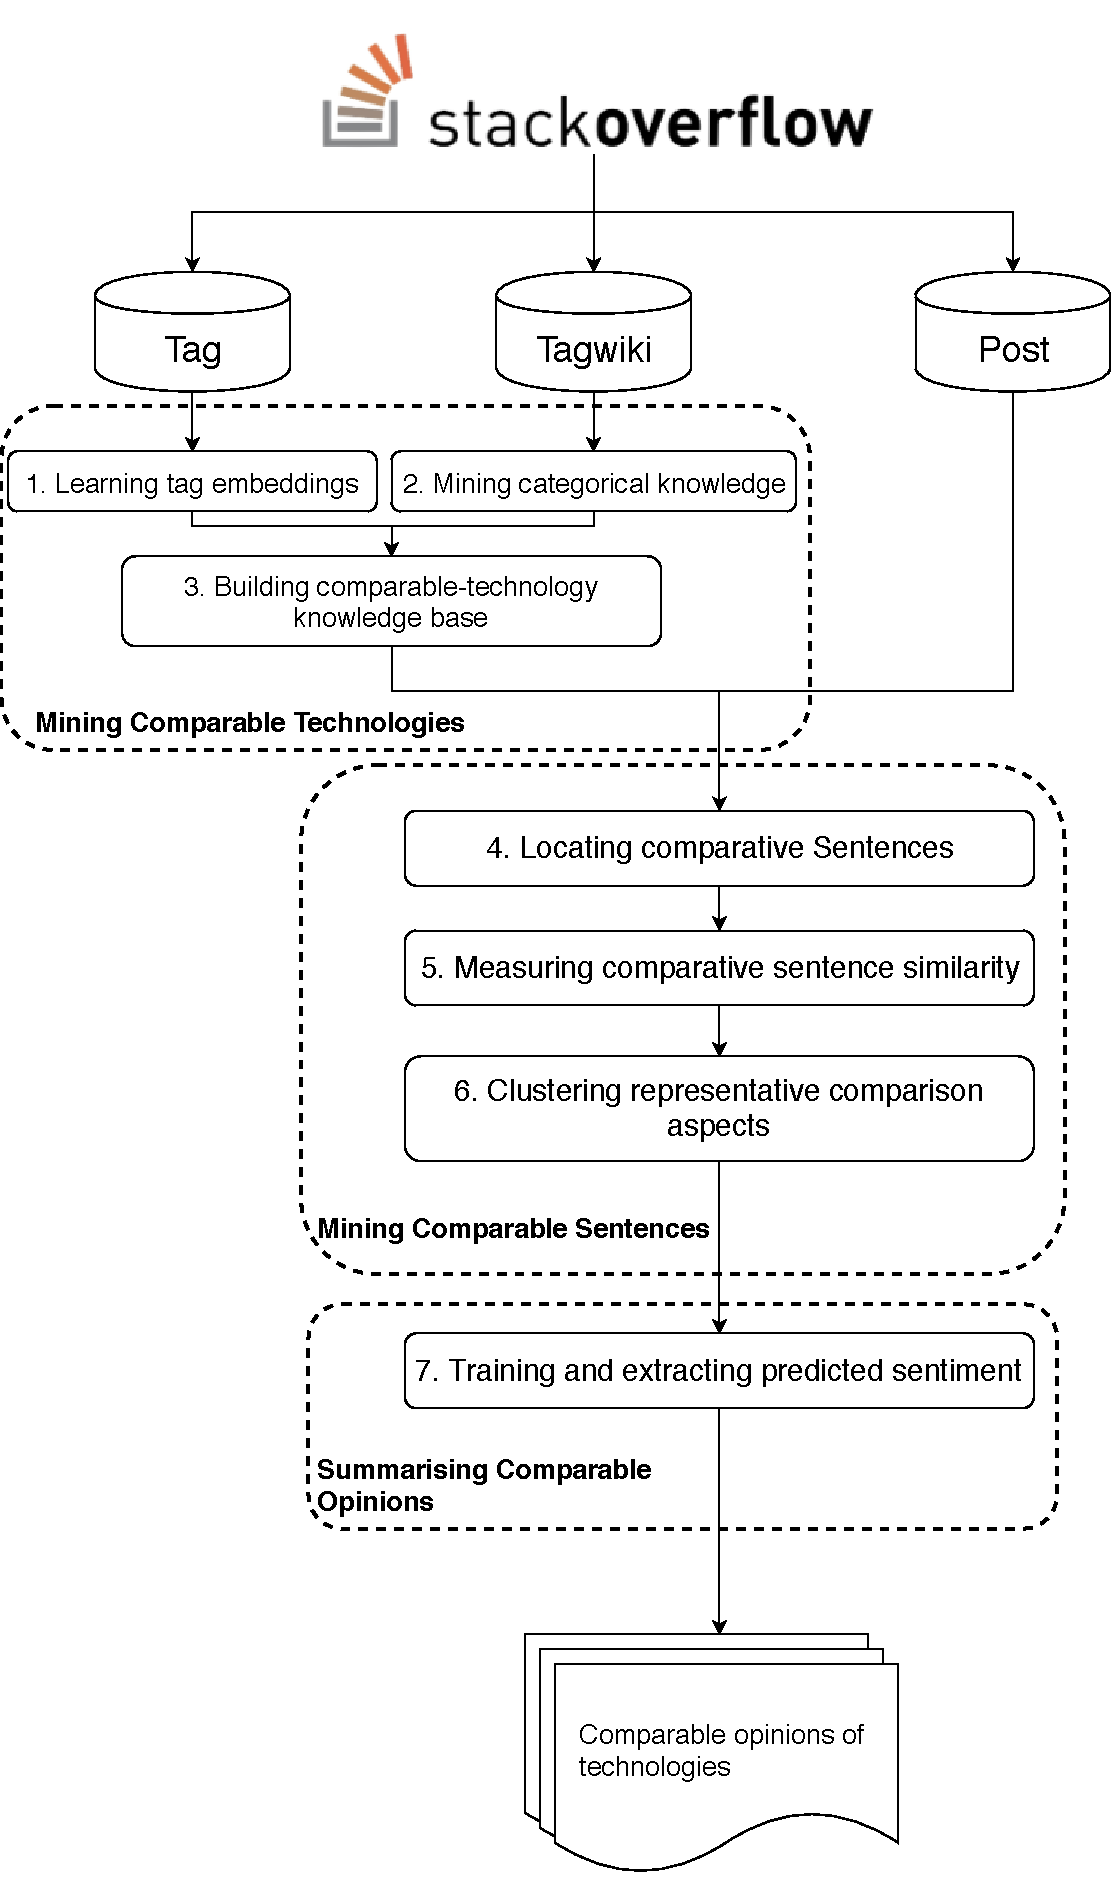
\includegraphics[width=0.48\textwidth]{figures/overview.pdf}
	\vspace{-4mm}
	\caption{The overview of our approach}
	\label{fig:overview}
	\vspace{-3mm}
\end{figure} 
%\section{Approach}
\label{sec:approach}

The overall structure of this section can follow my previous work~\cite{chen2017unsupervised}.

\subsection{Finding similar technique}

We find similar technique within Stack Overflow tags based on word embedding and categorical information.

\subsubsection{Learning Tag Embeddings}
\label{sec:w2v}

\begin{figure}
	\centering
	\subfigure[Continuous skip-gram model]{%
		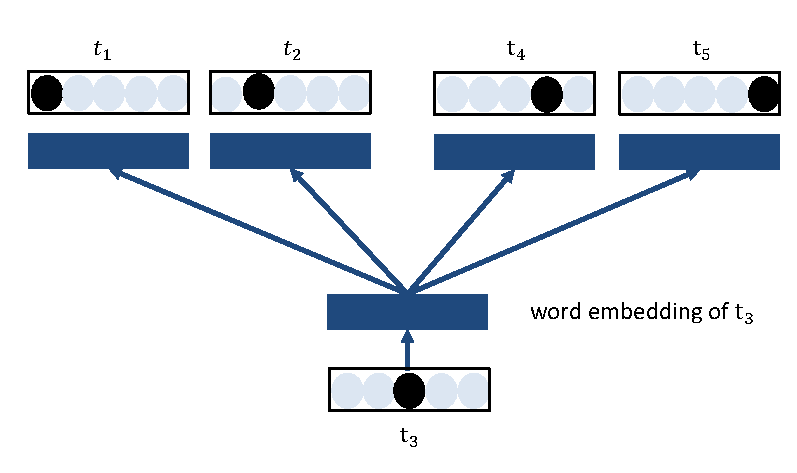
\includegraphics[width=0.23\textwidth]{figures/w2v_skip.pdf}
		\label{fig:w2v_skip}
	}
	\hfill
	\subfigure[Continuous bag-of-words model]{%
		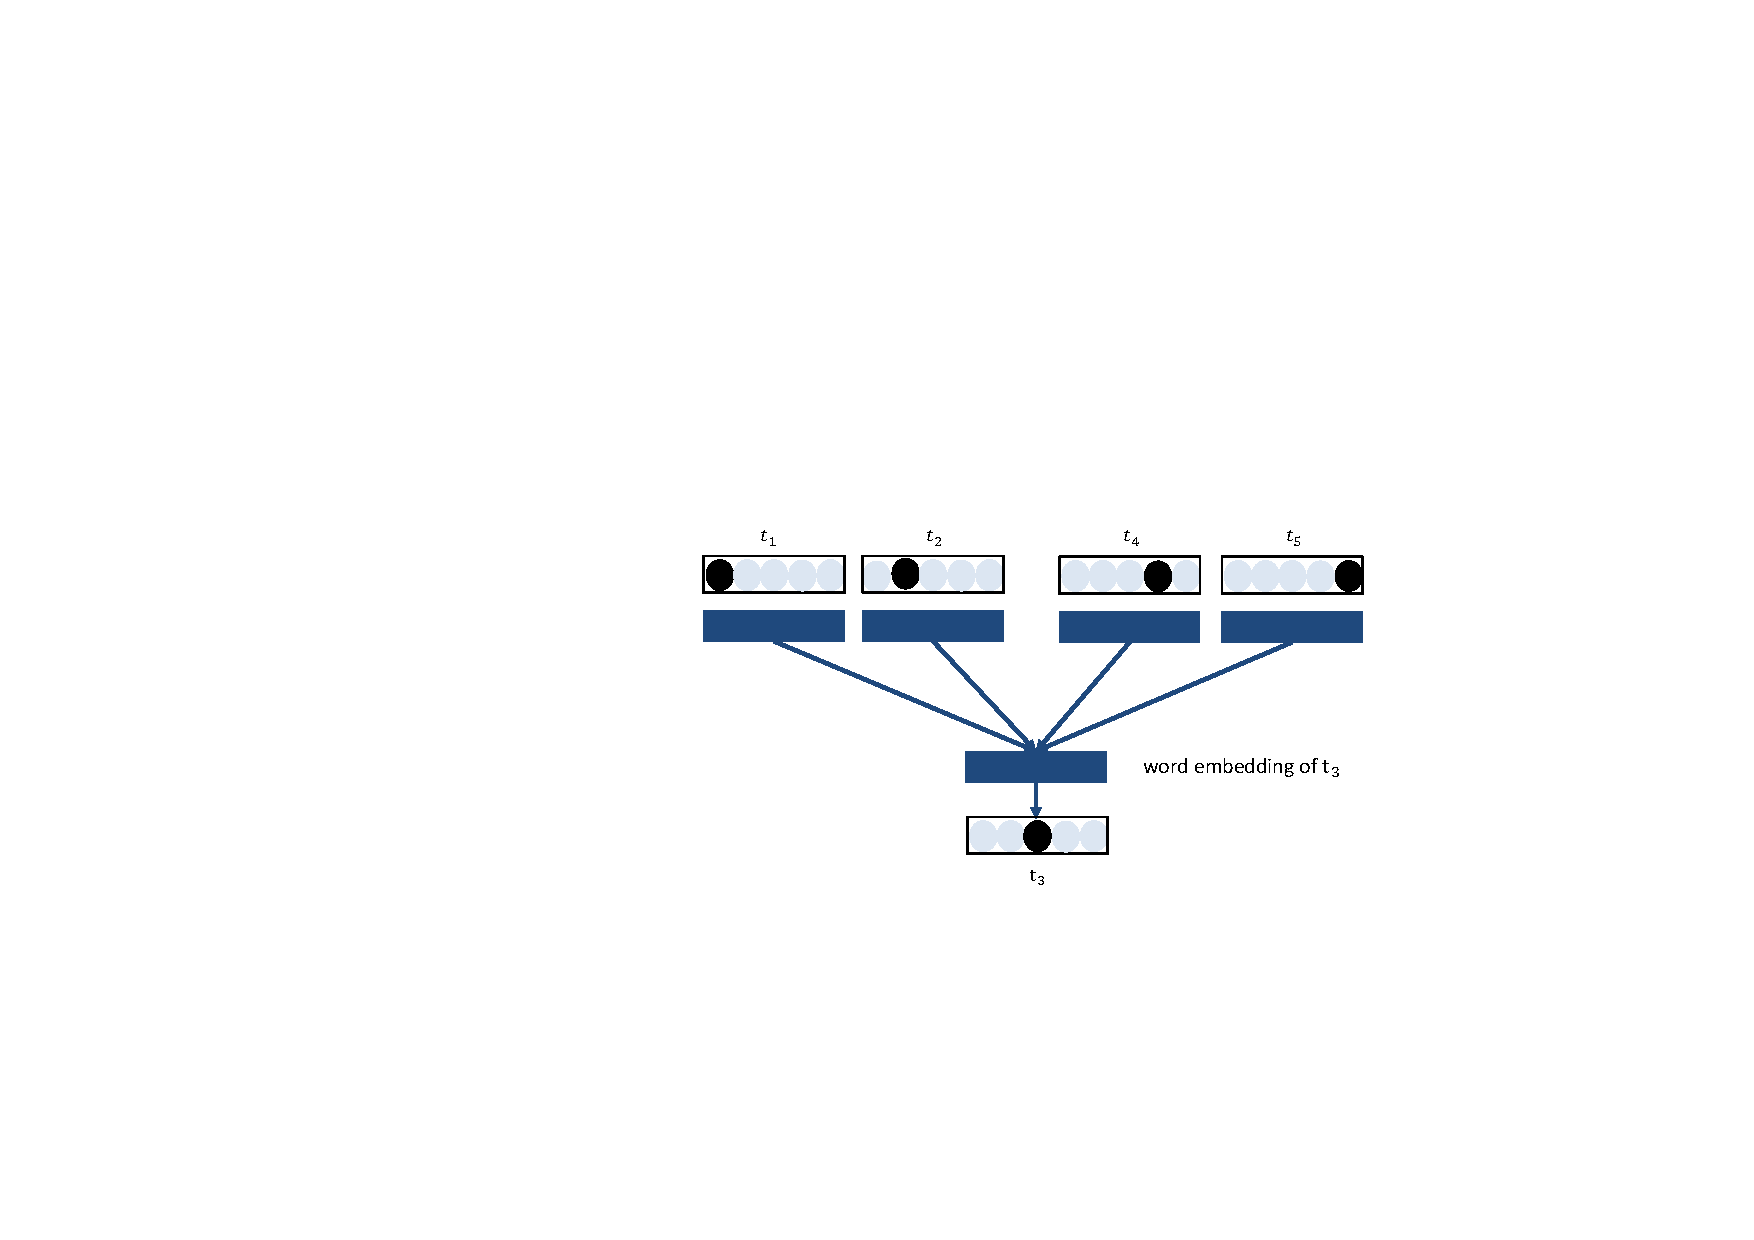
\includegraphics[width=0.23\textwidth]{figures/w2v_cbow.pdf}
		\label{fig:w2v_cbow}
	}
	\caption{The architecture of the two word embeddings models. The continuous skip-gram model predicts surrounding words given the central word, and the CBOW model predicts the central word based on the context words. Note the differences in arrow direction between the two models.
	}
	\label{fig:w2v}
\end{figure}

Word embeddings are dense low-dimensional vector representations of words that are built on the assumption that words with similar meanings tend to be present in similar context.
Studies~\cite{turian2010word, mikolov2013efficient} show that word embeddings are able to capture rich semantic and syntactic properties of words for measuring word similarity.
In our approach, given a corpus of tag sentences, we use word embedding methods to learn the word representation of each tag using the surrounding context of the tag in the corpus of tag sentences.


There are two kinds of widely-used word embedding methods~\cite{mikolov2013efficient}, the continuous skip-gram model~\cite{mikolov2013distributed} and the continuous bag-of-words (CBOW) model.
As illustrated in Fig.~\ref{fig:w2v}, the objective of the continuous skip-gram model is to learn the word representation of each word that is good at predicting the co-occurring words in the same sentence (Fig.~\ref{fig:w2v_skip}), while the CBOW is the opposite, that is, predicting the center word by the context words (Fig.~\ref{fig:w2v_cbow}).
Note that word order within the context window is not important for learning word embeddings.

Specifically, given a sequence of training text stream $t_{1}, t_{2}, ..., t_{k}$, the objective of the continuous skip-gram model is to maximize the following average log probability:
\begin{equation}
L = \frac{1}{K}\sum_{k=1}^{K} \sum_{-N\preceq j \preceq N, j\neq0} \log p(t_{k+j}|t_{k})
\label{equ:condition_skip}
\end{equation}
while the objective of the CBOW model is:
\begin{equation}
L = \frac{1}{K}\sum_{k=1}^{K} \log p(t_{k}|(t_{k-N}, t_{k-N+1}, ..., t_{k+N}) )
\label{equ:condition_cbow}
\end{equation}
where $t_{k}$ is the central word, $t_{k+j}$ is its surrounding word with the distance $j$, and $N$ indicates the context window size to be $2N+1$.
In our application of the word embedding, a tag sentence is a training text stream, and each tag is a word.
As tag sentence is short (has at most 5 tags), we set $N$ at 2 in our approach so that the context of one tag is all other tags in the current sentences.
That is, the context window contains all other tags as the surrounding words for a given tag.
Therefore, tag order does not matter in this work for learning tag embeddings.


The probability $p(t_{k+j}|t_{k})$ in Eq.~\ref{equ:condition_skip} or $p(t_{k}|(t_{k-j}, t_{k-j+1}, ..., t_{k+j}) )$ in Eq.~\ref{equ:condition_cbow} can be formulated as a log-linear softmax function which can be efficiently solved by the negative sampling method~\cite{mikolov2013distributed}.
After the iterative feed-forward and back propagation, the training process finally converges, and each tag obtains a low-dimension vector as its word representation (i.e., tag embedding) in the resulting vector space.

To determine which word-embedding model performs better in our analogical library reasoning task , we carry out a comparison experiment, and the details are discussed in Section~\ref{sec:comparison_w2v}.



\subsubsection{Mining Categorical Knowledge}

\label{sec:categoryKG}

\begin{figure}
	\centering
	\begin{tikzpicture}
	%\tikzset{level distance=1cm}
	%\tikzset{sibling distance=0.3cm}
	\tikzstyle{level 1}=[level distance=0.8cm, sibling distance=0.1cm]
	\tikzstyle{level 2}=[level distance=0.8cm, sibling distance=0.1cm]
	\tikzstyle{level 3}=[level distance=0.8cm, sibling distance=0.1cm]
	\tikzstyle{every node}=[font=\scriptsize]
	
	\Tree [.S [.NP [.NNS iOS ] ]
	[.VBZ is ]
	[.DT a ]
	[.JJ mobile ]
	[.NP [.NN operating ] [.NN system ] ]
	[.VBD developed ]
	[.IN by ]
	[.NP [.NNP Apple ] ]
	]
	
	\end{tikzpicture}
	\caption{POS tagging and phrase chunking results of the definition sentence of the tag \textit{iOS}}
	\label{fig:exampleChunking}
\end{figure}


In Fig.~\ref{fig:knowledgeGraph}, we can see that the tags can be of different categories, such as programming language, library, framework, tool, IDE, operating systems, etc.
To determine the category of a tag, we resort to the tag definition in the TagWiki of the tag.
The TagWiki of a tag is collaboratively edited by the Stack Overflow community.
Although there are no strict formatting rules in Stack Overflow, the TagWiki description usually starts with a short sentence to define the tag.
For example, the tagWiki of the tag \textit{iOS} starts with the sentence ``iOS is a mobile operating system developed by Apple''.
Typically, the first noun phrase just after the \textit{be} verb defines the category of the tag.
For example, from the tag definition of \textit{iOS}, we can learn that the category of \textit{iOS} is \textit{operating system}.
For the generality of our approach, we define \textit{noun phrase} in this work as a phrase consisting of consecutive nouns between other POS tags, including at least one noun.



Based on the above observation of tag definitions, we use the NLP methods (similar to the methods used in~\cite{kazama2007exploiting} for named entity recognition) to extract such noun phrase from the tag definition sentence as the category of a tag.
%The overview of extracting categorical knowledge can be seen in Figure.\ref{fig:flowChartCategory}.
Given the tagWiki of a tag in Stack Overflow, we extract the first sentence of the TagWiki description, and clean up the sentence by removing hyperlinks and brackets such as ``\{\}'', ``()''.
Then, we apply Part of Speech (POS) tagging and phrase chunking to the extracted sentence.
POS tagging is the process of marking up a word in a text as corresponding to a particular part of speech, such as noun, verb, adjective.
Phrase chunking is the process of segmenting a sentence into its subconstituents, such as noun phrases, verb phrases.
Different tools usually agree on the POS tags of nouns, and we find that POS tagger in NLTK~\cite{bird2006nltk}\footnote{\url{http://www.nltk.org/_modules/nltk/tag.html}} is especially suitable for our task.
In NLTK, the noun is annotated by different POS tags\footnote{\url{https://www.ling.upenn.edu/courses/Fall_2003/ling001/penn_treebank_pos.html}} including NN (Noun, singular or mass), NNS (Noun, plural), NNP (Proper noun, singular), NNPS (Proper noun, plural).
Then we use the phrase chunking i.e., regular expression to recognize consecutive nouns (at least one noun) as noun phrase by their POS tags.
%We adopt the default POS tagging and \textcolor{red}{??phrase chunking} implemented in NLTK\footnote{\url{http://www.nltk.org/_modules/nltk/tag.html}}.
%NLTK supports POS tags defined in the Penn Treebank Project\footnote{\url{https://www.ling.upenn.edu/courses/Fall_2003/ling001/penn_treebank_pos.html}}.
Fig.~\ref{fig:exampleChunking} shows the results for the tag definition sentence of \textit{iOS}.
Based on the POS tagging and phrase chunking results, we extract the first noun phrase (NP) (\textit{operating system} in this example) after the be verb (\textit{is} in this example).
We use this noun phrase as the category of the tag.
That is, the category of \textit{iOS} is \textit{operating system}.

With this method, we obtain 318 categories for the 23,658 tags (about 67\% of all the tags that have TagWiki).
We manually normalize these 318 categories labels, such as merging \textit{operating system} and \textit{os} as \textit{os}, \textit{libraries} and \textit{lib} as \textit{library}, and normalizing uppercase and lowercase (e.g., \textit{API} and \textit{api}).
As a result, we obtain 167 categories.
Furthermore, we manually categorize these 167 categories into four general categories: programming language, platform, library, and concept/standard.
These four general categories are defined in our previous work for named entity recognition~\cite{ye2016software}.
This generalization step is necessary, especially for the library tags that broadly refer to the tags whose fine-grained categories can be library, framework, api, toolkit, wrapper, and so on\footnote{A complete list can be found at \url{https://graphofknowledge.appspot.com/libCategory}}.
This is because the meaning of these fine-grained categories is often overlapping, and there is no consistent rule for the usage of these terms in the TagWiki.
For example, in Stack Overflow’s TagWiki, \textit{junit} is defined as a framework, \textit{google-visualization} is defined as an API, and \textit{wxpython} is defined as a wrapper. All these tags are referred to as library tags in our approach.


Although the above method obtains the tag category for the majority of the tags, the first sentence of the TagWiki of some tags is not formatted in the standard ``tag be noun phrase'' form.
For example, the first sentence of the TagWiki of the tag \textit{itext} is ``Library to create and manipulate PDF documents in Java'', or for \textit{markermanager}, the tag definition sentence is ``A Google Maps tool'', or for \textit{ghc-pkg}, the tag definition sentence is ``The command ghc-pkg can be used to handle GHC packages''.
As there is no \textit{be} verb in this sentence, the above NLP method cannot return a noun phrase as the tag category.
According to our observation, for most of such cases, the category of the tag is still present in the sentence, but often in many different ways.
It is very likely that the category word appears as the first noun phrase that match the existing category words in the definition sentence.
Therefore, we use a dictionary look-up method to determine the category of such tags.
Specially, we use the 167 categories obtained using the above NLP method as a dictionary to recognize the category of the tags that have not been categorized using the NLP method.
Given an uncategorized tag, we scan the first sentence of the tag's TagWiki from the beginning, and search for the first match of a category label in the sentence.
If a match is found, the tag is categorized as the matched category.
For example, the tag \textit{itext} is categorized as \textit{library} using this dictionary look-up method.
Using the dictionary look-up method, we obtain the category for 9,648 more tags.


Note that we cannot categorize some (less than 15\%) of the tags using the above NLP method and the dictionary look-up method.
This is because these tags do not have a clear tag definition sentence, for example, the TagWiki of the tag \textit{richtextbox} states that ``The RichTextBox control enables you to display or edit RTF content''.
This sentence is not a clear definition of what \textit{richtextbox} is.
Or no category match can be found in the tag definition sentence of some tags.
For example, the TagWiki of the tag \textit{carousel} states that ``A rotating display of content that can house a variety of content''.
Unfortunately, we do not have the category ``display'' in the 167 categories we collect using the NLP method.
When building analogical-libraries knowledge base, we exclude these uncategorized tags as potential candidates.

\subsubsection{Building similar-technology knowledge base}
Given a technology tag $t_1$ with its vector $vec(t_1)$, we first find most similar library $t_2$ whose vector $vec(t_2)$ is most closed to it, i.e.,
\begin{equation}
	\operatornamewithlimits{argmax}_{t_2 \in T}  \cos (vec(t_1), vec(t_2)) 
	\label{equ:similarity}
\end{equation} 
where $T$ is the set of technology tags excluding $t_1$, and $cos(u, v)$ is the cosine similarity of the two vectors.

\begin{table}
	\scriptsize
	\center	
	\begin{tabular}{l|l}
		\hline
		\textbf{Source Tech} & \textbf{Top-5 recommendations from word embedding} \\
		\hline
		nltk      & \textcolor{red}{\st{nlp}}, \textcolor{red}{\st{named-entity-recognition}}, opennlp, gate, \textcolor{red}{\st{language-model}} \\
				\hline
	\end{tabular}
	\vspace{1mm}
	\caption{Examples of filtering results by categorical knowledge (in red) \textcolor{red}{CCY: need to update with new examples}}
	\label{tab:filterResult}
\end{table}

Note that tags whose tag embedding is similar to the vector $vec(t_1)$ may not always be in the same category.
For example, tag embeddings of the tags \textit{word-sense-disambiguation}, \textit{pos-tagging} and \textit{sentiment-analysis} are similar to the vector $vec(nltk)$.
These tags are relevant to the \textit{nltk} library as they refer to some NLP concepts and tasks, but they are not analogical libraries to the \textit{nltk}.
In our approach, we rely on the category of tags (i.e., categorical knowledge) to return only tags within the same category as candidates.


In practice, there could be several similar technologies $t_2$ to the technology $t_1$.
Thus, we select tags $t_2$ with the cosine similarity in Eq.~\ref{equ:similarity} above a threshold $Thresh$.
Take the library \textit{nltk} (a NLP library in python) as an example.
We will preserve several candidates which are libraries such as \textit{textblob}, \textit{stanford-nlp}.

\subsection{Locating comparative sentences}
\textcolor{red}{Apart from Stack Overflow, we may also need to consider other related sites in Stack Exchange such as ask ubuntu, super user, unix \& linux, server fault, software engineering, software recommendation.}

\begin{table*}
	\centering
	\label{tab:pattern}
	\begin{tabular}{l l l l}
	\hline
	No. & Pattern & Sequence example & Original sentence \\ \hline \hline
	1 & \textit{TECH * VBZ * JJR} & jnnodb has 30 higher & innodb has 30 higher performance than myisam on average\\
	2 & \textit{TECH * VBZ * RBR} & post is more elegant & using post is more elegant and has more options for further development than passing them via get
\\
	3 & \textit{JJR * CIN * TECH} & slower than mysql & postgresql is slower than mysql especially when it comes to fine tuning in the end \\
	4 & \textit{RBR JJ * CIN TECH} & more powerful than velocity & freemarker is more powerful than velocity
 \\
	5 & \textit{CV * CIN TECH} & prefer ant over maven & i prefer ant over maven personally
\\
	6 & \textit{CV VBG TECH} & recommend using html5lib & i strongly recommend using html5lib instead of beautifulsoup
\\
	7 & \textit{CV TECH} & beat accurev & i have used svn cvs clearcase base ucm ccc harvest but none of them can beat accurev's strengths\\ \hline
	\end{tabular}
	\caption{The 7 comparative patterns. \textcolor{red}{CCY: 1)Please add the pattern ID at the first column. 2)For each pattern, why not consider both TECH1 and TECH2? 3)Add one column to show how many comparative sentences are extracted by this pattern. 4)replace the long examples with short sentences} }
\end{table*}

There are three steps to find comparative sentences of similar technologies.
We first carry out some preprocessing to the Stack Overflow data.
Then we locate the sentences that contain the name of any pair of similar technologies, and further spot the comparative sentences by checking if they satisfy the comparative patterns.
We will discuss these steps in detail in this section.

To extract convincing opinions about the comparison of similar technologies, we only consider answers with at least 1 score points.
Then we separate all convincing answers into individual sentences by punctuations like ``.'',  ``!'', ``?'', etc.
Note that we remove all questions sentences end with question mark, as we want to extract facts instead of doubts.
We lowercase all sentences to make them consistent with technology names because all tags are in lowercase.

\textcolor{red}{CCY: Give a table of some sample aliases}
To find sentences contain pairs of similar technologies, only using the tag names is not enough.
As posts in Stack Overflow are some informal discussion about programming-related issues, users may give different alias to the same thing.
For example, ``javascript'' can also be written in other forms such as ``js'', ``java-script'', ``javascrip'', etc.
So, aliases of software technologies are always abbreviations, synonyms, and some frequent misspellings in this work.
Such alias may lead to significant loss of comparative sentences.
Chen et al's work~\cite{chen2017unsupervised} built a large thesaurus of software-specific terms.
Based on their results, we find 7310 different alias for 3731 software technologies.
These aliases help find more potential comparative sentences.

To further identify comparative sentences from sentences containing similar technique, we propose a comparative pattern matching method. 
A sequence of POS tags is used to form a \textit{comparative pattern}. 
For example, ``\textit{RBR JJ IN}'' is a pattern that consists of a comparative adverb, a adjective and subsequently a preposition, such as "more efficient than", ``less friendly than'', etc. 
We extend the list of common POS tags to enhance the identification of comparative sentences.
More specifically, we create three comparative POS tags: \textit{CV} (comparative verbs, e.g. prefer, compare), \textit{CIN} (comparative prepositions, e.g. than, over) and \textit{TECH} (technology reference, including its name and aliases, e.g. python, eclipse).

Based on observations, we find that comparative sentences can be represented by some specific comparative patterns. 
We summarise 7 comparative patterns and corresponding examples in Table\ref{tab:pattern}.
To make the patterns more  flexible, we used a wildcard character to represent a list of arbitrary words. 
For each sentence containing similar technologies, we obtain their POS and check if any one of 7 patterns appear in them.
According to these comparative patterns, we can determine whether a sentence is a comparative sentence or not. 

\begin{comment}
The main process includes:
\begin{enumerate}
	\item Checking whether a sentence contains similar technique, including checking abbreviations and synonyms.
	\item Labeling all words in a sentence containing similar technique with common POS tags and our extended comparative POS tags;
	\item Using comparative patterns to match the sequence of POS tags. If the sentence matches at least one comparative pattern, we consider it as a comparative sentence.
\end{enumerate}}	
\end{comment}



\begin{comment}
\subsection{Extracting comparative opinions}
By analysing the sentence structure with Natural Language Processing, we extract the comparative relationships (like ``faster''), and relationship direction (like `` java --> python'').
So we transform the unstructured opinions into structured comparison. 

\subsubsection{Relationship extraction}
Observing the identified comparative sentences, we find that most of comparative relationships can be categorized into three patterns of POS tag sequence: RBR JJ (e.g. more powerful), JJR (e.g. faster) and JJR \textit{Noun} (e.g. better performance). Note that \textit{Noun} consists of NN, NNS, NNP and NNPS. We extract the part matching these three patterns in each sentence to represent the comparative relationship between the similar technique included in the sentence.
   
\subsubsection{Topic analysis}
In order to figure out what aspects of techniques users are concerned about, we conduct topic analysis based on the extracted relationships.
We use a keyword-based approach to analyze the topics. The relationships we extracted from comparative sentences are represented by ajectives (JJ), comparative adjectives (JJR) and nouns (NN, NNS, NNP and NNPS). Hence, we compile a list of keywords for each topic as Table 2 shows. The topic of each comparative sentence depends on whether this sentence contains at least one corresponding keyword.
\subsubsection{Preference Analysis} 
\end{comment}

\subsection{Extracting aspects}
After identifying comparative sentences, we extract the aspects of comparisons to summarize the comparative opinions. We utilize Word Mover's Distance to build graph for each similar technique pair and use community detection to classify comparative sentences. 
\subsubsection{Word Mover's Distance}
Word Mover's Distance (WMD) is a novel tool that allows us to accurately measure the similarity between two sentences. As Fig. ~\ref{fig:wmd} shows, the two sentences, ``\textit{postgresql} offers more security functionality than \textit{mysql}'' and "\textit{mysql} provides less safety features than \textit{postgresql}" have no words in common, but the "traveling distance" between them is small. WMD calculates the minimum amount of required distance "moving" from the embedded words of one sentence to the embedded words of another sentence~\cite{kusner2015word}. For normalization, we use WMD similarity that is simply the negative distance. For each comparative sentence, we use POS tags to extract adjectives (JJ), comparative adjectives (JJR) and nouns (NN, NNS, NNP and NNPS) as keywords to calculate WMD similarity. If the WMD similarity between comparative sentences exceeds the specified threshold, the two sentences would be added as two nodes and a linking edge to the graph for each similar technique pair. The threshold is not fixed and it depends on the difference between numbers of the extracted keywords.
\subsubsection{Community Detection}
After building graph for each similar technique pair, we use Givan-Newman algorithm to detect communities in the graph. The Givan-Newman algorithm is a hierarchical method and hence allows us to control the size of each detected community~\cite{girvan2002community}. We keep the size of communities for each similar technique pair appropriate based on the total number of comparative sentences. For each detected community, we extract the words with highest TF-IDF values as the aspect.

\begin{figure}
	\centering
	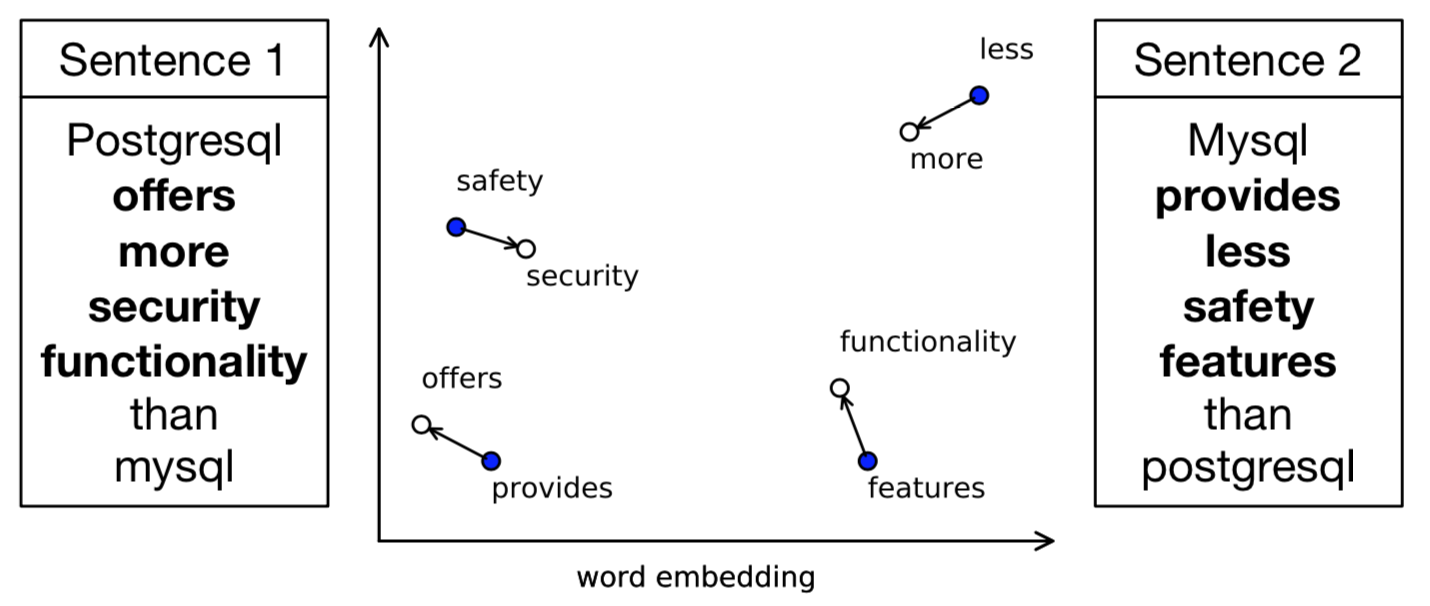
\includegraphics[width=0.5\textwidth]{figures/wmd.pdf}
	\label{fig:wmd}
	\caption{An illustration of the word mover's distance}
\end{figure}}

\subsection{Organizing the overall comparison}
We need to aggregate all individual opinions into an overview, so that users can obtain a more direct understanding of the different between the similar technique.
\section{Mining Similar Technology}
\label{sec:similarTech}

%We find comparable technologies by incorporating categorical information into word embedding of Stack Overflow tags.

Studies~\cite{barua2014developers, chen2016mining, treude2011programmers} show that Stack Overflow tags identify computer programming technologies that questions and answers revolve around. 
They cover a wide range of technologies, from algorithms (e.g.,  \textit{dijkstra, rsa}), programming languages (e.g., \textit{golang, javascript}), libraries and frameworks (e.g.,  \textit{gson, flask}), and development tools (e.g., \textit{sublime, vmware}). 
In this work, we regard Stack Overflow tags as a collection of technologies that developers would like to compare. 
We leverage word embedding techniques to infer semantically related tags, and develop natural language methods to analyze each tag's TagWiki to determine the corresponding technology's category (e.g., algorithm, library, IDE).
Finally, we build a knowledge base of comparable technologies by filtering the same-category, semantically-related tags. 

\subsection{Learning Tag Embeddings}
\label{sec:w2v}

\begin{figure}
	\centering
	\subfigure[Continuous skip-gram model]{%
		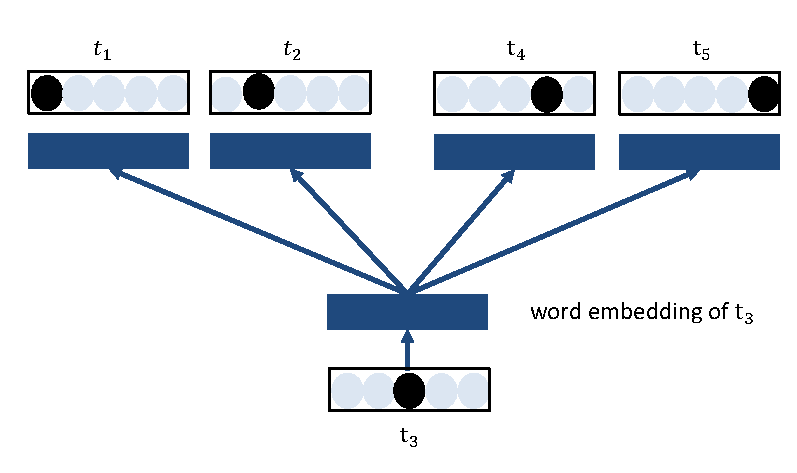
\includegraphics[width=0.23\textwidth]{figures/w2v_skip.pdf}
		\label{fig:w2v_skip}
	}
	\hfill
	\subfigure[Continuous bag-of-words model]{%
		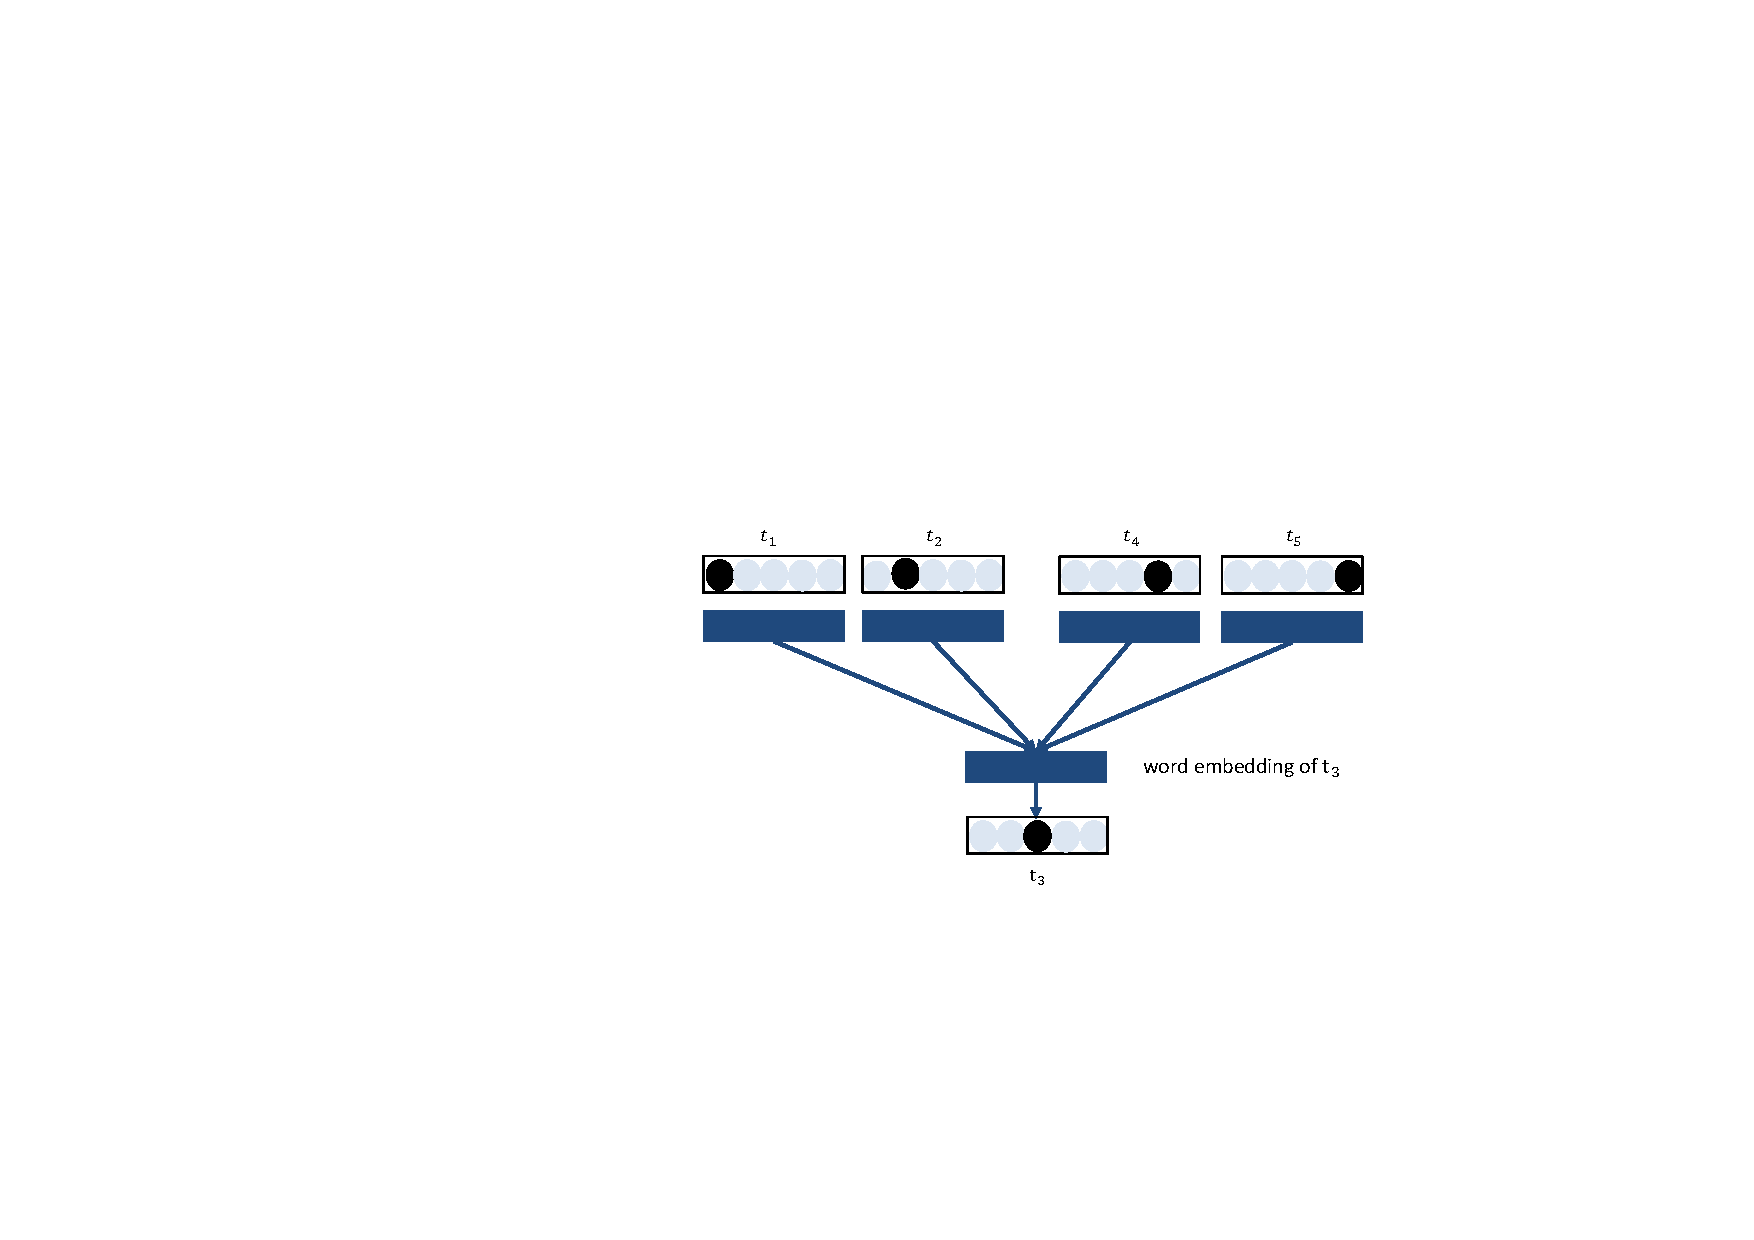
\includegraphics[width=0.23\textwidth]{figures/w2v_cbow.pdf}
		\label{fig:w2v_cbow}
	}
	\caption{The architecture of the two word embeddings models. The continuous skip-gram model predicts surrounding words given the central word, and the CBOW model predicts the central word based on the context words. Note the differences in arrow direction between the two models.
	}
	\vspace{-2mm}
	\label{fig:w2v}
\end{figure}

Word embeddings are dense low-dimensional vector representations of words that are built on the assumption that words with similar meanings tend to be present in similar context.
Studies~\cite{chen2016mining, mikolov2013efficient} show that word embeddings are able to capture rich semantic and syntactic properties of words for measuring word similarity.
In our approach, given a corpus of tag sentences, we use word embedding methods to learn the word representation of each tag using the surrounding context of the tag in the corpus of tag sentences.


There are two kinds of widely-used word embedding methods~\cite{mikolov2013efficient}, the continuous skip-gram model~\cite{mikolov2013distributed} and the continuous bag-of-words (CBOW) model.
As illustrated in Fig.~\ref{fig:w2v}, the objective of the continuous skip-gram model is to learn the word representation of each word that is good at predicting the co-occurring words in the same sentence (Fig.~\ref{fig:w2v_skip}), while the CBOW is the opposite, that is, predicting the center word by the context words (Fig.~\ref{fig:w2v_cbow}).
Note that word order within the context window is not important for learning word embeddings.

Specifically, given a sequence of training text stream $t_{1}, t_{2}, ..., t_{k}$, the objective of the continuous skip-gram model is to maximize the following average log probability:
\begin{equation}
L = \frac{1}{K}\sum_{k=1}^{K} \sum_{-N\preceq j \preceq N, j\neq0} \log p(t_{k+j}|t_{k})
\label{equ:condition_skip}
\end{equation}
while the objective of the CBOW model is:
\begin{equation}
L = \frac{1}{K}\sum_{k=1}^{K} \log p(t_{k}|(t_{k-N}, t_{k-N+1}, ..., t_{k+N}) )
\label{equ:condition_cbow}
\end{equation}
where $t_{k}$ is the central word, $t_{k+j}$ is its surrounding word with the distance $j$, and $N$ indicates the window size.
In our application of the word embedding, a tag sentence is a training text stream, and each tag is a word.
As tag sentence is short (has at most 5 tags), we set $N$ as 5 in our approach so that the context of one tag is all other tags in the current sentences.
That is, the context window contains all other tags as the surrounding words for a given tag.
Therefore, tag order does not matter in this work for learning tag embeddings.

\begin{comment}
The probability $p(t_{k+j}|t_{k})$  or $p(t_{k}|(t_{k-j}, t_{k-j+1}, ..., t_{k+j}) )$ in Eq.~\ref{equ:condition_skip} and Eq.~\ref{equ:condition_cbow} can be formulated as a log-linear softmax function which can be efficiently solved by the negative sampling method~\cite{mikolov2013distributed}.
After the iterative feed-forward and back propagation, the training process finally converges, and each tag obtains a low-dimension vector as its word representation (i.e., tag embedding) in the resulting vector space.	
\end{comment}
To determine which word-embedding model performs better in our comparable technology reasoning task , we carry out a comparison experiment, and the details are discussed in Section~\ref{sec:comparison_w2v}.



\subsection{Mining Categorical Knowledge}

\label{sec:categoryKG}

\begin{comment}
\begin{figure}
	\centering
	\begin{tikzpicture}
	%\tikzset{level distance=1cm}
	%\tikzset{sibling distance=0.3cm}
	\tikzstyle{level 1}=[level distance=0.8cm, sibling distance=0.1cm]
	\tikzstyle{level 2}=[level distance=0.8cm, sibling distance=0.1cm]
	\tikzstyle{level 3}=[level distance=0.8cm, sibling distance=0.1cm]
	\tikzstyle{every node}=[font=\scriptsize]
	
	\Tree [.S [.NP [.NNS iOS ] ]
	[.VBZ is ]
	[.DT a ]
	[.JJ mobile ]
	[.NP [.NN operating ] [.NN system ] ]
	[.VBD developed ]
	[.IN by ]
	[.NP [.NNP Apple ] ]
	]
	
	\end{tikzpicture}
	\caption{POS tagging and phrase chunking results of the definition sentence of the tag \textit{iOS} \textcolor{red}{Change this example}}
	\label{fig:exampleChunking}
\end{figure}	
\end{comment}

\begin{figure}
	\centering
	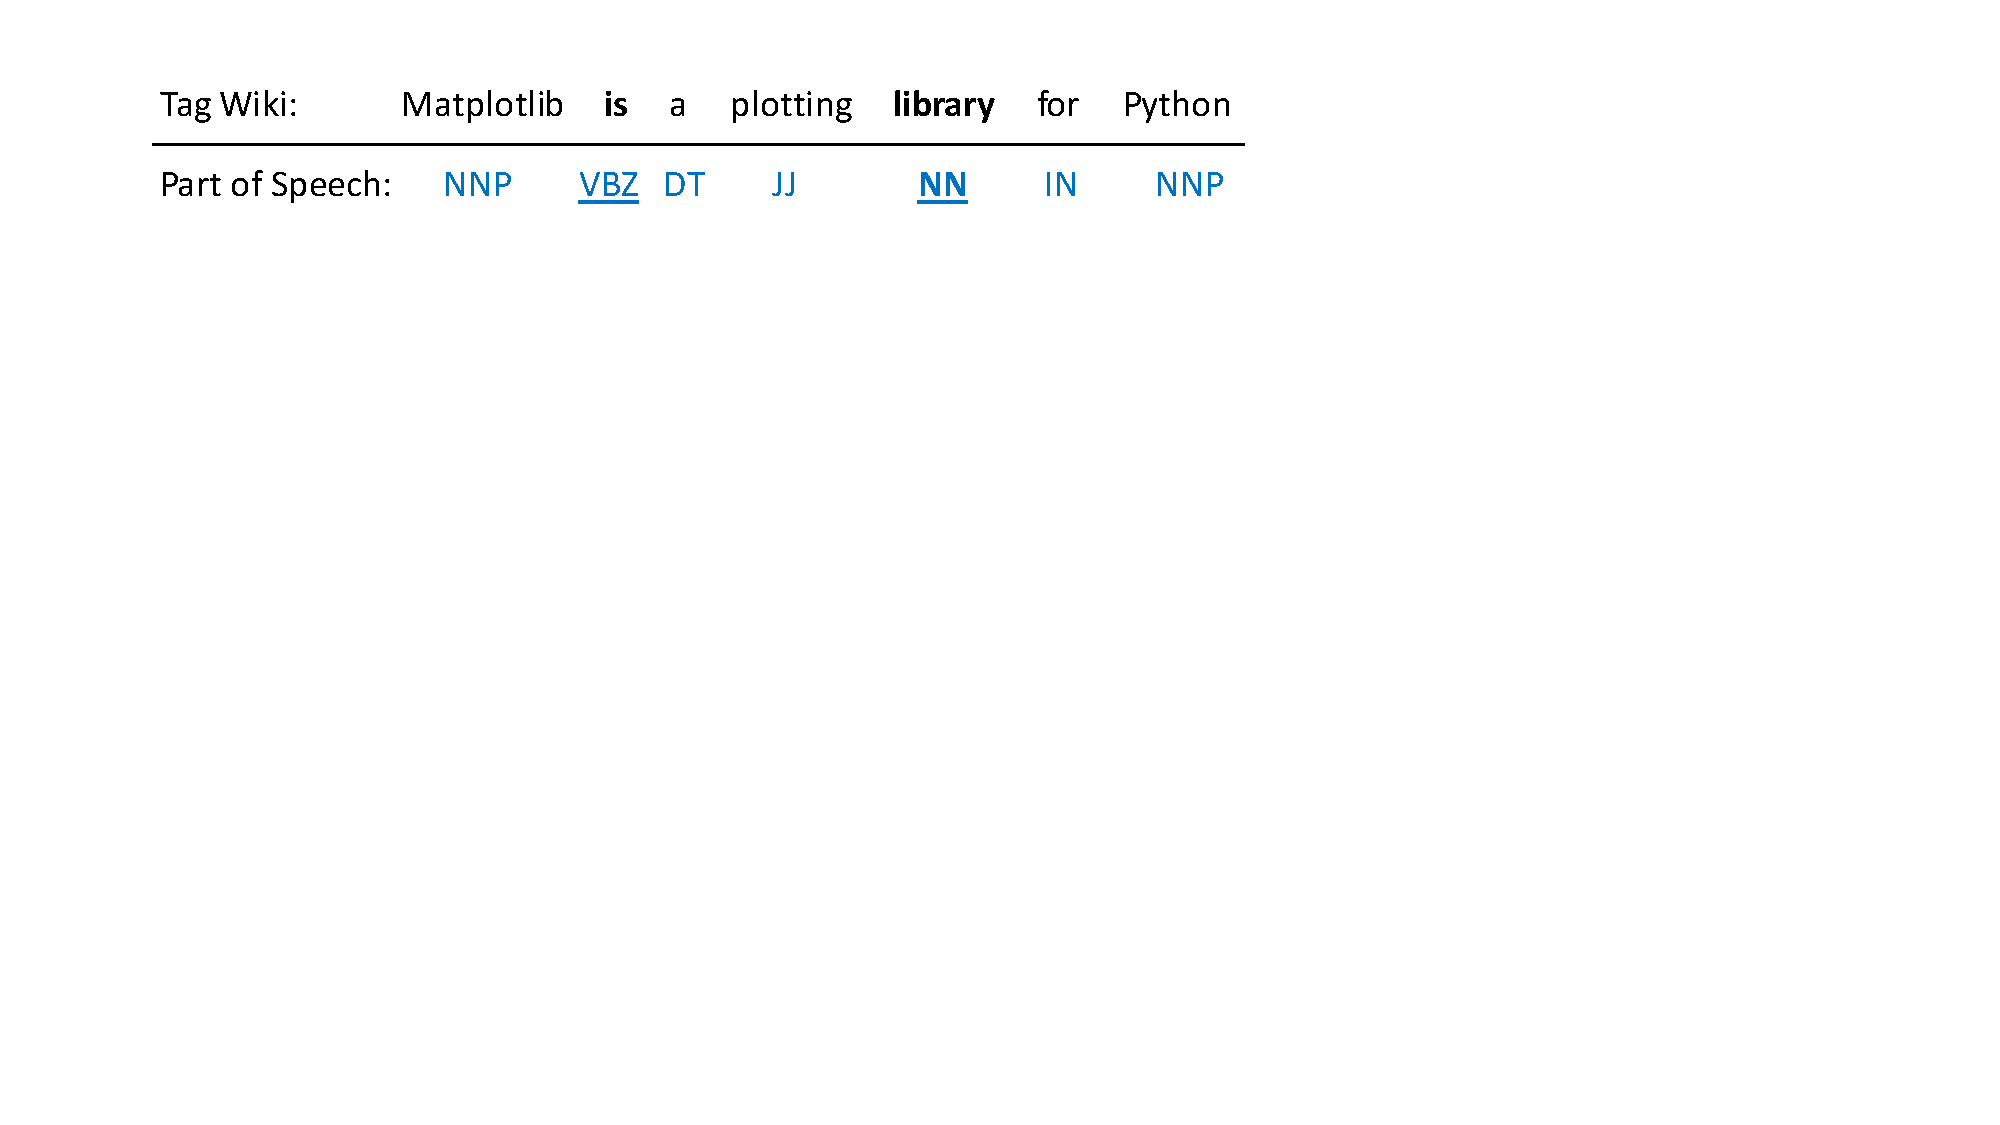
\includegraphics[width=0.46\textwidth]{figures/pos.pdf}
	\vspace{-3mm}
	\caption{POS tagging of the definition sentence of the tag \textit{RSA}}
	\vspace{-2mm}
	\label{fig:exampleChunking}
\end{figure}
In Stack Overflow, tags can be of different categories, such as programming language, library, framework, tool, API, algorithm, etc.
To determine the category of a tag, we resort to the tag definition in the TagWiki of the tag.
The TagWiki of a tag is collaboratively edited by the Stack Overflow community.
Although there are no strict formatting rules in Stack Overflow, the TagWiki description usually starts with a short sentence to define the tag.
For example, the tagWiki of the tag \textit{Matplotlib} starts with the sentence ``Matplotlib is a plotting library for Python''.
Typically, the first noun just after the \textit{be} verb defines the category of the tag.
For example, from the tag definition of \textit{Matplotlib}, we can learn that the category of \textit{Matplotlib} is \textit{library}.

Based on the above observation of tag definitions, we use the NLP methods~\cite{kazama2007exploiting, chen2016mining} to extract such noun from the tag definition sentence as the category of a tag.
%The overview of extracting categorical knowledge can be seen in Figure.\ref{fig:flowChartCategory}.
Given the tagWiki of a tag in Stack Overflow, we extract the first sentence of the TagWiki description, and clean up the sentence by removing hyperlinks and brackets such as ``\{\}'', ``()''.
Then, we apply Part of Speech (POS) tagging to the extracted sentence.
POS tagging is the process of marking up a word in a text as corresponding to a particular part of speech, such as noun, verb, adjective.
%Phrase chunking is the process of segmenting a sentence into its subconstituents, such as noun phrases, verb phrases.
NLP tools usually agree on the POS tags of nouns, and we find that POS tagger in NLTK~\cite{bird2004nltk} is especially suitable for our task.
In NLTK, the noun is annotated by different POS tags~\cite{web:nltktag} including NN (Noun, singular or mass), NNS (Noun, plural), NNP (Proper noun, singular), NNPS (Proper noun, plural).
%Then we use the phrase chunking i.e., regular expression to recognize consecutive nouns (at least one noun) as noun phrase by their POS tags.
%We adopt the default POS tagging and \textcolor{red}{??phrase chunking} implemented in NLTK\footnote{\url{http://www.nltk.org/_modules/nltk/tag.html}}.
%NLTK supports POS tags defined in the Penn Treebank Project\footnote{\url{https://www.ling.upenn.edu/courses/Fall_2003/ling001/penn_treebank_pos.html}}.
Fig.~\ref{fig:exampleChunking} shows the results for the tag definition sentence of \textit{RSA}.
Based on the POS tagging results, we extract the first noun  (\textit{algorithm} in this example) after the be verb (\textit{is} in this example) as the category of the tag.
That is, the category of \textit{RSA} is \textit{algorithm}.
Note that if the noun is some specific words such as \textit{system}, \textit{development}, we will further check its neighborhood words to see if it is \textit{operating system} or \textit{independent development environment}.

With this method, we obtain 318 categories for the 23,658 tags (about 67\% of all the tags that have TagWiki).
We manually normalize these 318 categories labels, such as merging \textit{app} and \textit{applications} as \textit{application}, \textit{libraries} and \textit{lib} as \textit{library}, and normalizing uppercase and lowercase (e.g., \textit{API} and \textit{api}).
As a result, we obtain 167 categories.
Furthermore, we manually categorize these 167 categories into five general categories: programming language, platform, library, API, and concept/standard~\cite{ye2016software}.
This is because the meaning of the fine-grained categories is often overlapping, and there is no consistent rule for the usage of these terms in the TagWiki.
This generalization step is necessary, especially for the library tags that broadly refer to the tags whose fine-grained categories can be library, framework, api, toolkit, wrapper, and so on.
%\footnote{A complete list can be found at \url{https://graphofknowledge.appspot.com/libCategory}}
For example, in Stack Overflow's TagWiki, \textit{junit} is defined as a framework, \textit{google-visualization} is defined as an API, and \textit{wxpython} is defined as a wrapper. 
All these tags are referred to as library tags in our approach.


Although the above method obtains the tag category for the majority of the tags, the first sentence of the TagWiki of some tags is not formatted in the standard ``tag be noun phrase'' form.
For example, the first sentence of the TagWiki of the tag \textit{itext} is ``Library to create and manipulate PDF documents in Java'', or for \textit{markermanager}, the tag definition sentence is ``A Google Maps tool'', or for \textit{ghc-pkg}, the tag definition sentence is ``The command ghc-pkg can be used to handle GHC packages''.
As there is no \textit{be} verb in this sentence, the above NLP method cannot return a noun phrase as the tag category.
According to our observation, for most of such cases, the category of the tag is still present in the sentence, but often in many different ways.
It is very likely that the category word appears as the first noun phrase that match the existing category words in the definition sentence.
Therefore, we use a dictionary look-up method to determine the category of such tags.
Specially, we use the 167 categories obtained using the above NLP method as a dictionary to recognize the category of the tags that have not been categorized using the NLP method.
Given an uncategorized tag, we scan the first sentence of the tag's TagWiki from the beginning, and search for the first match of a category label in the sentence.
If a match is found, the tag is categorized as the matched category.
For example, the tag \textit{itext} is categorized as \textit{library} using this dictionary look-up method.
Using the dictionary look-up method, we obtain the category for 9,648 more tags.

Note that we cannot categorize some (less than 15\%) of the tags using the above NLP method and the dictionary look-up method.
This is because these tags do not have a clear tag definition sentence, for example, the TagWiki of the tag \textit{richtextbox} states that ``The RichTextBox control enables you to display or edit RTF content''.
This sentence is not a clear definition of what \textit{richtextbox} is.
Or no category match can be found in the tag definition sentence of some tags.
For example, the TagWiki of the tag \textit{carousel} states that ``A rotating display of content that can house a variety of content''.
Unfortunately, we do not have the category ``display'' in the 167 categories we collect using the NLP method.
When building comparable-technologies knowledge base, we exclude these uncategorized tags as potential candidates.

\subsection{Building Similar-technology Knowledge Base}
Given a technology tag $t_1$ with its vector $vec(t_1)$, we first find most similar library $t_2$ whose vector $vec(t_2)$ is most closed to it, i.e.,
\begin{equation}
	\operatornamewithlimits{argmax}_{t_2 \in T}  \cos (vec(t_1), vec(t_2)) 
	\label{equ:similarity}
\end{equation} 
where $T$ is the set of technology tags excluding $t_1$, and $cos(u, v)$ is the cosine similarity of the two vectors.

\begin{table}
	\small
	\center	
	\caption{Examples of filtering results by categorical knowledge (in red)}
	\vspace{-2mm}
	\setlength{\tabcolsep}{0.2em}
	\begin{tabular}{l|l}
		\hline
		\textbf{Source} & \textbf{Top-5 recommendations from word embedding} \\
		\hline
		nltk   & \textcolor{red}{\st{nlp}}, opennlp, gate, \textcolor{red}{\st{language-model}}, stanford-nlp \\
		tcp    & tcp-ip, \textcolor{red}{\st{network-programming}}, udp, \textcolor{red}{\st{packets}}, \textcolor{red}{\st{tcpserver}} \\
		vim    & sublimetext, \textcolor{red}{\st{vim-plugin}}, emacs, nano, gedit\\
		swift  & objective-c, \textcolor{red}{\st{cocoa-touch}}, \textcolor{red}{\st{storyboard}}, \textcolor{red}{\st{launch-screen}} \\%,\textcolor{red}{\st{asset-catalog}} \\
		%unicode & gbk, utf, 
		bubble-sort & insertion-sort, selection-sort, mergesort, timsort, heapsort \\
				\hline
	\end{tabular}
	\vspace{-3mm}
	\label{tab:filterResult}
\end{table}

Note that tags whose tag embedding is similar to the vector $vec(t_1)$ may not always be in the same category.
For example, tag embeddings of the tags \textit{nlp}, \textit{language-model} are similar to the vector $vec(nltk)$.
These tags are relevant to the \textit{nltk} library as they refer to some NLP concepts and tasks, but they are not comparable libraries to the \textit{nltk}.
In our approach, we rely on the category of tags (i.e., categorical knowledge) to return only tags within the same category as candidates.
Some examples can be seen in Table~\ref{tab:filterResult}.


In practice, there could be several comparable technologies $t_2$ to the technology $t_1$.
Thus, we select tags $t_2$ with the cosine similarity in Eq.~\ref{equ:similarity} above a threshold $Thresh$.
Take the library \textit{nltk} (a NLP library in python) as an example.
We will preserve several candidates which are libraries such as \textit{textblob}, \textit{stanford-nlp}.
\section{Mining Comparative Opinions}


%2) According to the word embedding, can we adopt better clustering methods?



For each pair of comparable technologies in the knowledge base, we analyze the Q\&A discussions in Stack Overflow to extract plausible comparative sentences by which Stack Overflow users express their opinions on the comparable technologies. 
\revise{Note that the comparison of comparable technologies may lie in one sentence, but also consecutive sentences.
So, we also take the context into consideration for comparison opinion extraction.}
%\wang{Sometimes users express their opinion in one simple comparative sentence, and sometimes they tend to compare technology pairs in two sentences respectively. Either way, we may obtain many comparative sentences for each pair of comparable technologies.}
Displaying all these sentences as a whole may make it difficult for developers to read and digest the comparison information.
Therefore, we measure the similarity among the comparative sentences, and then cluster them into several groups, each of which may identify a prominent aspect of technology comparison that users are concerned with.
%The extracted comparative sentences are clustered to reveal the prominent aspects that users are concerned with when comparing the two technologies.

\subsection{Extracting Comparative Sentences}
\label{sec:comparativeSentence}

There are three steps to extract comparative sentences of the two technologies.
We first carry out some preprocessing of the Stack Overflow post content.
Then we locate the sentences that contain the name of the two technologies, and further select the comparative sentences that satisfy a set of comparative sentence patterns.

\subsubsection{Preprocessing}
To extract trustworthy opinions about the comparison of technologies, we consider only answer posts with positive score points.
Then we split the textual content of such answer posts into individual sentences by punctuations like ``.'',  ``!'', ``?''.
We remove all sentences ended with question mark, as we want to extract facts instead of doubts. 
We further exclude sentences from question post, as most of them are assumptions or questions to ask.
We lowercase all sentences to make the sentence tokens consistent with the technology names because all tags are in lowercase. 
\begin{figure}
	\centering
	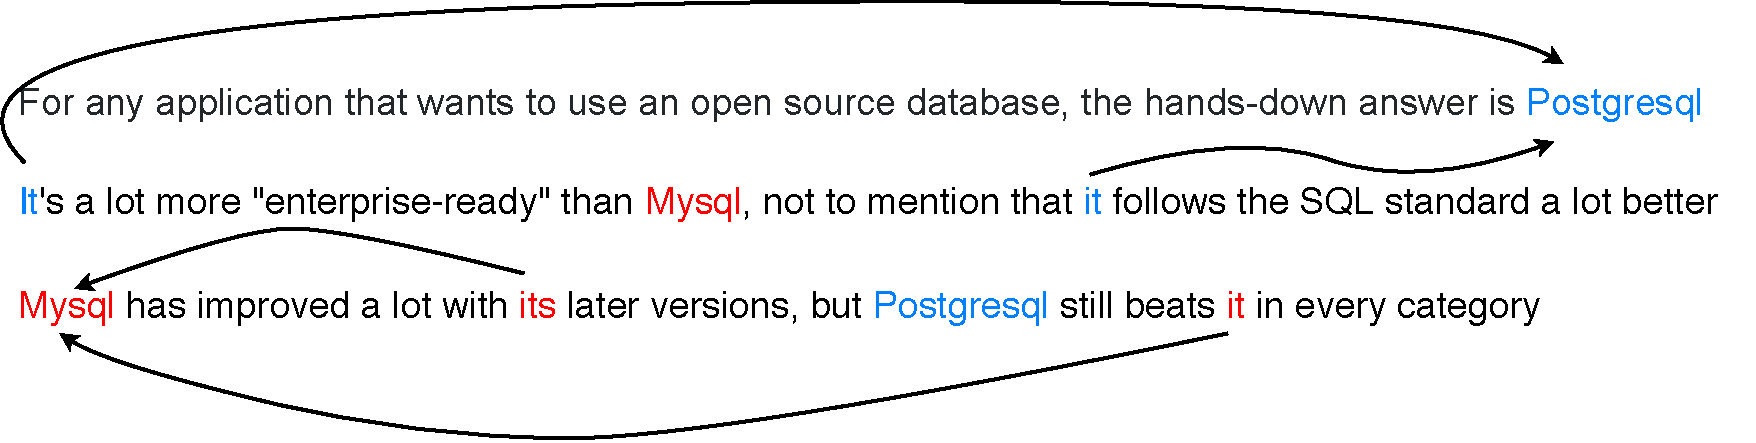
\includegraphics[width=0.47\textwidth]{figures/coreference.pdf}
	\vspace{1mm}
	\caption{An example of coreference resolution in comparative sentence.}
	\label{fig:coreference}
	\vspace{-3mm}
\end{figure}

\revise{Note that within the technical discussion in Stack Overflow, developers may adopt some pronoun like ``it'', ``that'', ``which'' to represent the technology.
For example, given the paragraph ``\textit{For any application that wants to use an open source database, the hands-down answer is postgresql. It's a lot more enterprise-ready than mysql, not ot mention that it follows the SQL standard a lot better. Mysql has improved a lot with its later versions, but Postgresql still beats it in every category.}'' as seen in Figure~\ref{fig:coreference}, the two ``it'' in the second sentence refers to ``postgresql'' in the first sentence. 
But with some cases, the reference may be too far from its source, leading to the negative influence to the location of comparative sentences. 
Therefore, we adopt the coreference resolution algorithm~\cite{clark2016deep} to recover the pronoun before locating comparative sentences.}

\revise{Conventionally, the coreference resolution is based on a set of manual-crafted rules by analyzing dependency tree of words in the sentence.
However, those rules may not be scalable, therefore, we adopt the state-of-the-art neural network based coreference method, named NeuralCoref\footnote{\url{https://github.com/huggingface/neuralcoref}}.
It feeds word embedding of potential words around each mention to two neural networks with one for giving score for finding a possible antecedent, and the other giving a score for a mention having no antecedent.
Given two scores, we compare them and pick the highest score to determine whether the mention has an antecedent and which word it is.}
  
\begin{comment}
\wang{We adopt the coreference method from NeuralCoref~\cite{}(site the github page?or medium page). The method extracts the mentions and potential antecedents by parsing sentences with spaCy parser~\cite{honnibal2015improved} first. Then it uses trained word embedding model, which was trained on the OntoNotes 5.0 dataset\cite{ralph2012ontonotes}, to tokenize pairs of mentions. The method includes the neural mention-ranking model\cite{clark2016deep}, which takes in the words vectors and some additional features(i.e. length of mentions, location of metnions...) as input. The input gets through four hidden layers of fully connected neural nets with rectified linear (ReLU) activation functions~\cite{nair2010rectified}, and the output links the the mention with its highest scored antecedent.  They apply the ranking model into two neural nets. One net is to give a score for each pair or mention and its possible antecedent, the other net is to give a score of the mention that doesn't have antecedents. Finally, given two scores, the method compares them and pick the highest score to determine whether the mention has an antecedent and which word it is. }
%\wang{We also use Coreference technique to preprocess sentences that contains tech pairs. The Coreference resolution can annotate sentence clusters and help us replace the pronoun with its corresponding subject, which should be helpful for us to locate and select comparative sentences in the following sections. Fig \ref{fig:coreference} shows that the Corefrerence reads that \textit{It} in the second sentence refers to the \textit{Postgresql} in the first sentece. So we further change the \textit{It} to \textit{Postgresql}, which makes it matches Pattern 2 for Single sentence.} 
\end{comment}



\subsubsection{Locating Candidate Sentences}
\revise{The sentences mentioning a pair of comparable technologies may contain the comparison opinion of them.
According to our observation, the comparison may occur in either one single sentence, or the contextual sentences.
Therefore, the candidate comparison sentences may be single sentences mentioning two comparable technologies, or the consecutive sentences with each of it containing one comparable technology respectively.
}

Note that using only the tag names is not enough.
As posts in Stack Overflow are informal discussions about programming-related issues, users often use alias to refer to the same technology.
Aliases of technologies can be abbreviations, synonyms and some frequent misspellings.
\revise{For example, there are several different alias of ``visual studio'' in many forms such as ``visual-studio'' (synonym), ``vs'' (abbreviation), and ``visual studion'' (misspelling) in the discussions.}
The presence of such aliases will lead to significant missing of comparative sentences, if we match technology mentions in a sentence with only tag names.
Chen et al.'s work~\cite{chen2019sethesaurus} builds a large thesaurus of morphological forms of software-specific terms, including abbreviations, synonyms and misspellings.
Table~\ref{tab:alias} shows some examples of technologies aliases in this thesaurus.
Based on this thesaurus, we find 7310 different alias for 3731 software technologies.
These aliases help to locate more candidate comparative sentences that mention certain technologies.

\begin{table}
	\scriptsize
	\center	
	\caption{Examples of alias}
	\vspace{-4mm}
	%\setlength{\tabcolsep}{0.3em}
    \setlength{\tabcolsep}{0.1em}
	\begin{tabular}{c c c}
		\hline
		\textbf{Tech term} & \textbf{Synonyms} & \textbf{Abbreviation} \\
		\hline
		photoshop & adobe\_photoshop, photoshops & ps \\
		dataframe & data-frame, pd.dataframe & df \\
		libgd &  gd\_library & gd \\		
        microsoft sql server & ms-sql, msql, ms\_sql & mssql \\
        		breadth-first search & breadth first search, breadth-first-search & bfs \\
				\hline
	\end{tabular}
	\vspace{-3mm}
	\label{tab:alias}
\end{table}

\subsubsection{Selecting Comparative Sentences}
%\textcolor{blue}{Not all sentences mentioning the two technologies are comparative sentences, for example, ... give an example ...}.
To identify comparative sentences from candidate sentences, we develop two sets of comparative sentence patterns: \revise{one for the single sentence and the other for contextual sentences.} 
Single sentence pattern is a sequence of POS tags. 
For example, the sequence of POS tags ``\textit{RBR JJ IN}'' is a pattern that consists of a comparative adverb (\textit{RBR}), an adjective (\textit{JJ}) and subsequently a preposition (\textit{IN}), such as "more efficient than", ``less friendly than'', etc. 
We extend the list of common POS tags to enhance the identification of comparative sentences.
More specifically, we create four comparative POS tags: \textit{CV} (comparative verbs, e.g. prefer, compare, beat), \textit{CIN} (comparative prepositions, e.g. than, over), \textit{NW} (negation words, e.g. wouldn't, doesn't ), and \textit{TECH} (technology reference, including the name and aliases of a technology, e.g. python, eclipse).

\begin{table*}
	\centering
	\caption{\revise{Patterns of comparative single sentences} \chen{1. Please change the examples 2. For each pattern, should we have both TECHs appearing in each pattern?}}
	\vspace{-3mm}
% 	\setlength{\tabcolsep}{0.1em}
\renewcommand{\arraystretch}{1.2}
	\textbf{Single sentence} 
	\begin{tabular}{l|l|l|l}
		\hline 
		\textbf{No.} & \textbf{Pattern} & \textbf{Sequence example} & \textbf{Original sentence} \\ \hline
		1 & \textit{TECH * VBZ * (JJR} $\lor$\textit{ RBR)} & innodb has 30 higher & InnoDB has 30\% higher performance than MyISAM on average. \\ \hline
		\multirow{2}{*}{2} & \multirow{2}{*}{\textit{((RBR JJ) } $\lor$\textit{ JJR) * CIN * TECH}} & faster than coalesce & Isnull is faster than coalesce. \\
		& & more complex than mysql & Triggers in postgresql have a syntax a bit more complex than mysql. \\ \hline
		3 & \textit{CV * CIN TECH} & recommend scylla over cassandra  & I would recommend scylla over cassandra. \\ \hline
		4 & \textit{CV VBG TECH} & recommend using html5lib & I strongly recommend using html5lib instead of beautifulsoup. \\
		\hline 
		%7 & \textit{CV TECH} & beat accurev & I have used svn, cvs,  clearcase but none of them can beat accurev's strengths\\ 
		%\vspace{1mm}	
	\end{tabular}
	
	\vspace{-3mm}
	\label{tab:patternSingle}
\end{table*}

%we find that comparative sentences can be represented by some specific comparative patterns.
Based on data observations of comparative sentences, we summarise four comparative patterns for single sentences as seen in Table~\ref{tab:patternSingle}.
To make the patterns more flexible, we use a wildcard character to represent a list of arbitrary words to match the pattern. 
For each sentence mentioning the two comparable technologies, we obtain its POS tags and check if it matches any one of four patterns.
If so, the sentence will be selected as a single comparative sentence.

\revise{For contextual candidate sentences, we develop three patterns for identifying comparative opinions in Table~\ref{tab:patternMultiple}. First, ... Second, ...}
\wang{The first two patterns are similar to the first two patterns in single sentence. Instead, those sentences tend to split the comparable technologies into each sentence respectfully. So we collect those sentences mentioned both of the comparable technology pairs, check if one of them match the POS tags pattern and the other sentence is using the second technology as a subject or an object, then we find a match.}
\chen{The first two patterns are further needed for discussion as there is some obvious flaw with it. For example, what if one sentence contain the pattern, the other sentence is not related to the pattern?}
\revise{The other pattern is that one contextual sentences is the affirmation (AFF) while the other is negation (NEG) with at least one comparable technology appears as the subject of one sentence.
For example, the prior sentence ``Cassini does not support HTTPs'' is the negation sentence, and the latter sentence ``However, you can use IIS to do this'' is the affirmation sentence, resulting in the comparison opinion that IIS can support the feature that is not owned by Cassini.}
\chen{How do we know one sentence is positive while the other is negative, and this example is not very good.}
\wang{In order to extract the \textit{AFF-NEG} pattern, We firstly create a list of negation words defined as ``\textit{NW}'' in POS tag. For each pair of sentences we check if either of them match the pattern ``\textit{TECH NW}'',so that we locate the negation sentence. Then, for the other sentence, we make sure it contains the other comparative tag and match the following one of the pattern:``\textit{TECH VB NN}'', ``\textit{TECH VB JJ}'', ``\textit{TECH VB RB}'', and ``\textit{VB TECH TO VB}''. All of which are making sure the other sentence is a affirmation sentence talking about the comparative tag. If the selected pair of sentences match the rules we talked above, we select them as \textit{AFF-NEG} pattern comparative sentences.  }

%\wang{During the process of exploring and observing real data, we find out that users also tend to describe a tech pair in two sentences, so we further develop the Contextual sentence. For two contextual sentences, if they contain two comparable technologies respectfully, and either of them match the first 2 patterns, we select them as contextual comparative sentence. For the \textit{POS-NEG} pattern, we collect sentences that contain comparable technologies but have different semantic statements, whereas one is positive the other is negative. Table~\ref{tab:pattern} shows these patterns and the corresponding examples of comparative sentences. s}
%According to these comparative patterns, we can determine whether a sentence is a comparative sentence or not. 


\begin{table*}
	\centering
	\caption{\revise{Patterns of comparative contextual sentences} \chen{1. The first two patterns need to be further discussed. 2. Please preserve the original style of the example}}
	\begin{tabular}{l|l|l|l}
		\hline 
		\textbf{No.} & \textbf{Pattern} & \textbf{Sequence example} & \textbf{Original sentence} \\ \hline
		\multirow{2}{*}{1} & \multirow{2}{*}{ \textit{TECH * VBZ * (JJR} $\lor$\textit{ RBR)}} & \multirow{2}{*}{triple des is generally better} & Triple des is generally better but there are some known theoretical attacks. \\ & & & If you have a choice of cipher you might want to look at aes instead. \\
		\hline
		\multirow{2}{*}{2} & \multirow{2}{*}{\textit{((RBR JJ) } $\lor$\textit{ JJR) * CIN * TECH}} & \multirow{2}{*}{faster than MySQL}  & Postgres has a richer set of abilities and a better optimizer.\\& & &  Its ability to do hash joins often makes it much faster than MySQL for joins. \\
		\hline
		\multirow{2}{*}{3} & \multirow{2}{*}{\textit{AFF | NEG}} & cassini does not & Cassini does not support https. \\ & &iis to do  & However you can use iis to do this.
		
	\end{tabular}
	\label{tab:patternMultiple}
\end{table*}


\subsection{Measure Sentence Similarity}
\label{sec:measuresimilarity}
\begin{comment}
So we have a word embedding matrix $X ∈ R^{(d \times n)}$ with $d$ as the embedding size of one word, and $n$ as the vocabulary size.
The $i^{th}$ column, $v_i ∈ R^d$, represents the embedding of the $i^{th}$
word in $d$-dimensional space. 
We assume text sentences are represented as normalized bag-of-words vectors, $S ∈ R^{n}$. 
To be precise, if word $i$ appears $f_i$ times in the sentence, we denote $S_i = \frac{f_i}{\sum^{n}_{j=1}f_j}$.
\end{comment}

To measure the similarity of two comparative sentences, we adopt the Word Mover's Distance~\cite{kusner2015word} which is especially useful for short-text comparison.
%\textcolor{blue}{... one sentence to explain the key idea of Word Mover's Distance ...}
Given two sentences $S_1$ and $S_2$, we take one word $i$ from $S_1$ and one word $j$ from $S_2$.
Let their word vectors be $v_i$ and $v_j$.
The distance between the word $i$ and the word $j$ is the Euclidean distance between their vectors, $c(i, j) = ||v_i - v_j||_2$.
To avoid confusion between word and sentence distance, we will refer to $c(i, j)$ as the cost associated with ``traveling'' from one word to another.
%Let $T \subseteq R^{n \times m}$ be a (sparse) flow matrix where $n$ and $m$ are the number of words of sentence $S_1$ and $S_2$ respectively.
One word $i$ in $S_1$ may move to several different words in the $S_2$, but its total weight is 1.
So we use $T_{ij} \geq 0$ to denote how much of word $i$ in $S_1$ travels to word $j$ in $S_2$.
%To transform $S_1$ entirely into $S_2$, we ensure that the entire outgoing flow from word $i$ equals $S_i$, i.e., $\sum_j T_{ij} = S_i$
It costs $\sum_j T_{ij}c(i,j)$ to move one word $i$ entirely into $S_2$.
We define the distance between the two sentences as the minimum (weighted) cumulative cost required to move all words from $S_1$ to $S_2$, i.e., $D(S_1, S_2) = \sum_{i,j} T_{ij}c(i,j)$.
This problem is very similar to transportation problem i.e., how to spend less to transform all goods from source cities $A_1, A_2, ...$ to target cities $B_1, B_2, ...$.
Getting such minimum cost actually is a well-studied optimization problem of earth mover distance~\cite{ling2007efficient, pele2009fast}.
%We allow each word $i$ in $S_1$ to be transformed into any word in $S_2$ \textcolor{blue}{in total or in parts ??mean what? ``all or some words in $S_2$? I do not think we really need to mention this. This really depends on the input sentence representation. If we do not use initial sentences but only subsequence containing words to be compared, then we can alway have all to all}. 

\begin{figure}
	\centering
	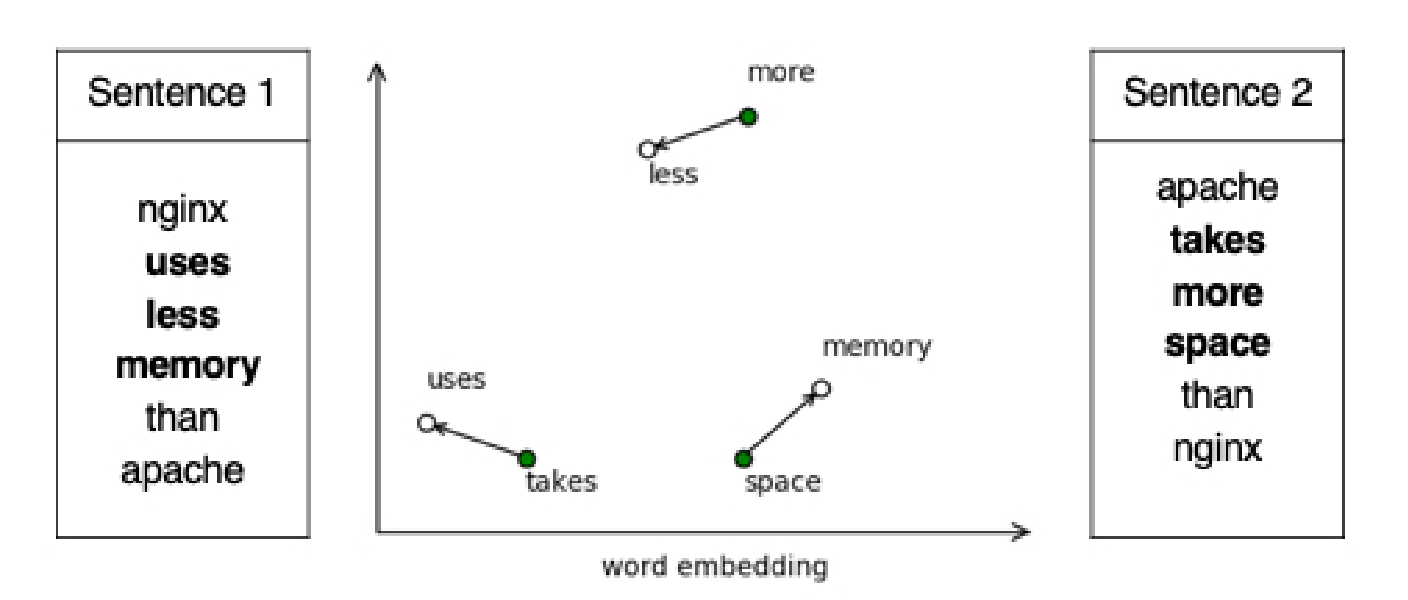
\includegraphics[width=0.49\textwidth]{figures/wmd1.pdf}
	\vspace{-7mm}
	\caption{An illustration of measuring similarity of two comparative sentences \chen{Please use the PDF file.}}
	\vspace{-3mm}
	\label{fig:wmd}
\end{figure}

To use word mover's distance in our approach, we first train a word embedding model based on the post content of Stack Overflow so that we get a dense vector representation for each word in Stack Overflow.
Word embedding has been shown to be able to capture rich semantic and syntactic information of words.
Our approach does not consider word mover's distance for all words in a sentence.
Instead, for each comparative sentence, we extract only keywords with POS tags that are most relevant to the comparison, including adjectives (JJ), comparative adjectives (JJR) and nouns (NN, NNS, NNP and NNPS), not including the technologies under comparison. 
Then, we compute the minimal word movers' distance between the keywords in one sentence and those in the other sentences.
Base on the distance, we further compute the similarity score of the two sentences by 
$$ similarity \ score (S_1, S_2) = \frac{1}{1+D(S_1, S_2)} $$
The similarity score is in range $(0, 1)$, and the higher the score, the more similar the two sentences.
If the similarity score between the two sentences is larger than the threshold, we regard them as similar.
The threshold is 0.55 in this work, determined heuristically by a small-scale pilot study. 
We show some similar comparative sentences by word mover's distance in Table~\ref{tab:wmd}.

To help reader understand word movers' distance, we show an example in Figure~\ref{fig:wmd} with two comparative sentences for comparing \textit{apache} and \textit{nginx}: ``\textit{nginx uses less memory than apache}'' and ``'\textit{Apache takes more space than nginx}'.
The keywords in the two sentences that are most relevant to the comparison are highlighted in bold.
We see that the minimum distance between the two sentences is mainly the accumulation of word distance between pairs of similar words \textit{(uses, takes)}, \textit{(less, more)}, and \textit{(memory, space)}. 
%If we consider the distance between other pairs of words, such as \textit{(security, less)}, \textit{(offer, functionality)}, the overall distance would be much larger.
As the distance between the two sentences is small, the similarity score is high even though the two sentences use rather different words and express the comparison in reverse directions.

\begin{comment}
Word Mover's Distance (WMD) is a novel tool that allows us to accurately measure the similarity between two sentences. As Fig. ~\ref{fig:wmd} shows, apart from the technology names, the two sentences, ``\textit{postgresql} offers more security functionality than \textit{mysql}'' and ``\textit{mysql} provides less safety features than \textit{postgresql}'' have no words in common, but the "traveling distance" between them is small. WMD measures the minimum amount of required distance "moving" from the embedded words of one sentence to the embedded words of another sentence~\cite{kusner2015word}. For normalization, we compute WMD similarity that is simply the negative distance. For each comparative sentence, we use POS tagger to extract adjectives (JJ), comparative adjectives (JJR) and nouns (NN, NNS, NNP and NNPS) as candidate keywords. Then, we calculate WMD similarity based on the four candidate keywords near every technology. 
\end{comment}                                                     

\begin{table*}
	\centering
	\caption{Examples of similar comparative sentences by Word Mover's Distance}
	\vspace{-3mm}
	\begin{tabular}{l|l}
	\hline
	\textbf{Comparable technology pair} & \textbf{Comparative sentences} \\ \hline
	\multirow{2}{*}{\textit{quicksort} \& \textit{mergesort}} & Quicksort is done in place and doesn’t require allocating memory, unlike mergesort. \\ & Mergesort would use more space than quicksort. \\ \hline
	\multirow{2}{*}{\textit{swing} \& \textit{awt}} & Consider using swing which has much better performance over the old heavyweight awt. \\ & Yes swing has newer and better apis than awt. \\ \hline
	\multirow{2}{*}{\textit{google-chrome} \& \textit{safari}} & But safari takes more time than google-chrome browser. \\ &  I get a lot of results about how safari is slower than google-chrome. \\ \hline
	\multirow{2}{*}{\textit{get} \& \textit{post}} & Post is also more secure than get because you aren t sticking". \\ & When you use post data is a a lot more safer than get and you can send large no. of request parameters. \\ \hline
	\multirow{2}{*}{\textit{tcp} \& \textit{udp}} & Tcp is a slower more reliable protocol than udp is. \\ & This is the reason why udp is much faster than tcp. \\ \hline
	\end{tabular}
	\vspace{-1mm}
	\label{tab:wmd}
\end{table*}
	
\subsection{Clustering Representative Comparison Aspects}
For each pair of comparable technologies, we collect a set of comparative sentences about their comparison in Section~\ref{sec:comparativeSentence}.
Within these comparative sentences, we find pairs of similar sentences in Section~\ref{sec:measuresimilarity}.
We take each comparative sentence as one node in the graph.
If the two sentences are determined as similar, we add an edge between them in the graph.
In this way, we obtain a graph of comparative sentences for a given pair of comparative technologies.

\begin{figure}
	\centering
	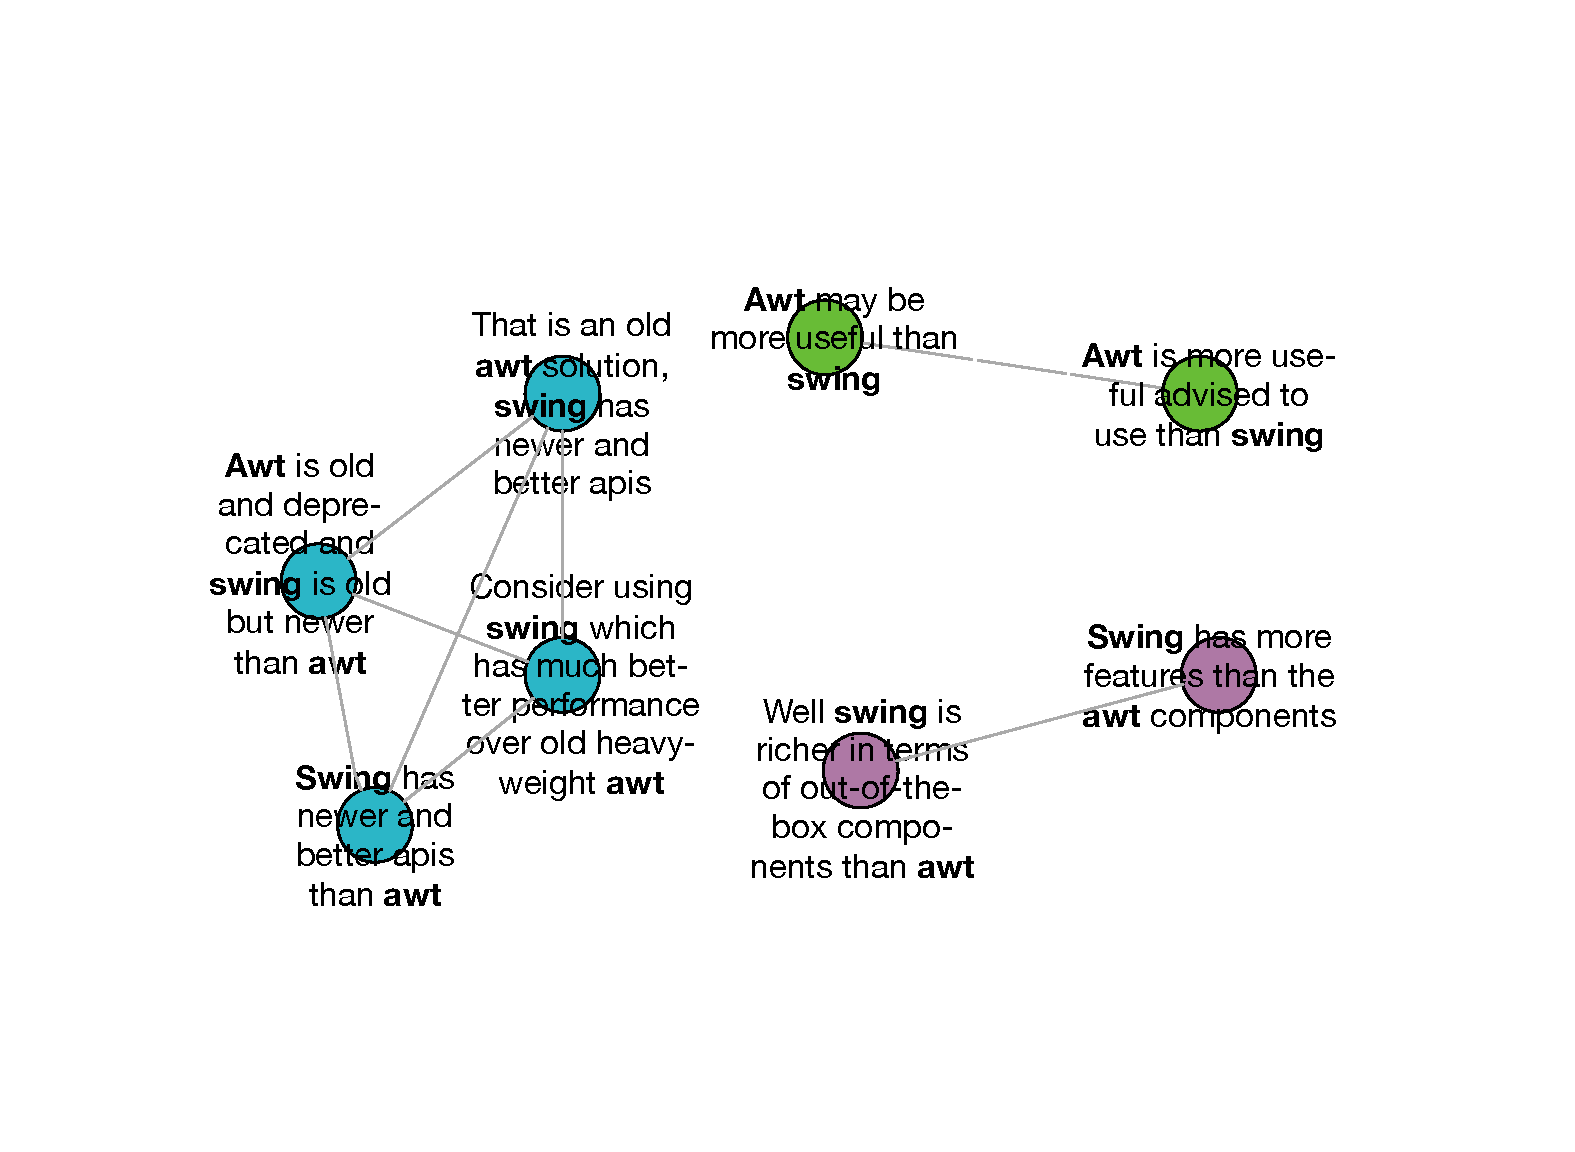
\includegraphics[width=0.45\textwidth]{figures/communities.pdf}
	\vspace{-6mm}
	\caption{Communities in the graph of comparative sentences \chen{This example does not show the power of community detection, as each subgraph is regarded as a community.}}
	\vspace{-3mm}
	\label{fig:communities}
\end{figure} 

Although some comparative sentences are very different in words or comparison directions (examples shown in Fig.~\ref{fig:wmd} and Table~\ref{tab:wmd}), they may still share the same comparison opinions.
In graph theory, a set of highly correlated nodes is referred to as a community (cluster) in the network.
Based on the sentence similarity, we cluster similar opinions by applying the community detection algorithm to the graph of comparative sentences.
In this work, we use the Girvan-Newman algorithm~\cite{girvan2002community} which is a hierarchical community detection method.
It uses an iterative modularity maximization method to partition the network into a finite number of disjoint clusters that will be considered as communities. 
Each node must be assigned to exactly one community.
Fig.~\ref{fig:communities} shows the graph of comparative sentences for the comparison of \textit{awt} and \textit{swing} (two java toolkits), in which each node is a comparative sentence, and the detected communities are visualized in the same color.
%Do we need to introduce the tricks that we use for our cases

As seen in Fig.~\ref{fig:communities}, each community may represent a prominent comparison aspect of the two comparable technologies.
But some communities may contain too many comparative sentences to understand easily.
Therefore, we use TF-IDF (Term Frequency Inverse Document Frequency) to extract keywords from comparative sentence in one community to represent the comparison aspect of this community.
TF-IDF is a statistical measure to evaluate the importance of a word to a document in a collection. 
It consists of two parts: term frequency (TF, the number occurrences of a term in a document) and inverse document frequency (IDF, the logarithm of the total number of documents in the collection divided by the number of documents in the collection that contain the specific term).
For each community, we remove stop words in the sentences, and regard each community as a document.
We take the top-3 words with largest TF-IDF scores as the representative aspect for the community.
Table~\ref{tab:aspects} shows the comparison aspects of four communities for comparing \textit{UDP} with \textit{TCP}.
The representative keywords directly show that the comparison between \textit{UDP} with \textit{TCP} mainly focuses on four aspects: speed, header, usability, and fields that they are used for.

\begin{table*}
	\centering
	\caption{The representative keywords for clusters of \textit{UDP} and \textit{TCP}.}
	\vspace{-3mm}
	\setlength{\tabcolsep}{0.01em}
	\begin{tabular}{l|l}
	\hline
	\textbf{Representative keywords} & \textbf{Comparative sentences} \\ \hline
	\multirow{3}{*}{faster slower reliable} & One often finds the argument that udp is faster then tcp \\ & Udp is way lighter and faster but somewhat less reliable than tcp. \\ & Udp is generally faster than tcp as it does not have to do the overhead checking of consistency that tcp must deal with.\\ \hline
	\multirow{3}{*}{header connection size} & You will notice that the tcp header has more fields than the udp header and many of those fields will be populated. \\ & Udp communication is connection less as compared to tcp which need a connection. \\ & The header size of udp is less than tcp. \\ \hline
	\multirow{3}{*}{harder, easier,travelsal} & Doing p2p nat traversal over tcp is a bit harder than udp. \\ & Keep in mind that implementing udp traversal is easier than tcp. \\ & It was introduced since the nat traversal for tcp is much more complicated than udp. \\ \hline
	%\multirow{3}{*}{better, protocol} & Udp is a lightweight protocol ;tcp is a better choice if you want robust packet delivery and sequencing. \\ & In general the tcp protocol manages the available network bandwidth better than the udp protocol. \\ & Udp scales better than tcp because of reduced states that need to be maintained in the operating system. \\ \hline
	\end{tabular}
	\vspace{-1mm}
	\label{tab:aspects}
\end{table*}


\begin{comment}
If the WMD similarity between comparative sentences exceeds a specified threshold, the two sentences would be added as two nodes and a linking edge to the graph for each similar technology pair. The threshold is not fixed and it depends on the difference between numbers of the extracted keywords. If a comparative sentence was not added to the graph, the sentence would be considered to belong to the ``others'' aspect.
	
After building graph for each similar technology pair, we use Givan-Newman algorithm to detect communities in the graph. The Givan-Newman algorithm is a hierarchical method and hence allows us to control the size of each detected community~\cite{girvan2002community}. We keep the size of communities for each similar technology pair appropriate based on the total number of comparative sentences.

In order to figure out what aspects of technologies users are concerned about, we extract the words with highest TF-IDF values as the aspect for each detected community.

Term frequency-inverse document frequency (TF-IDF) is a statistical measure that is intended to evaluate the importance of a word to a document in a collection. The TF-IDF consists of two parts: term frequency (TF, the number occurrences of a term in a document) and inverse document frequency (IDF, the logarithm of the total number of documents in the collection divided by the number of documents in the collection that contain the specific term). The TF measures the frequency of a term while the IDF reflects the importance of a term. Therefore, the higher TF-IDF value of a term demonstrates that the term is more important to the document.

In our scenario, we utilize the TF-IDF value to extract representative keywords for each clusters. For each comparative technology pair, we consider every cluster as a document and use all documents to form a collection. Then, we calculate the TF-IDF value for each candidate keyword and extract at most three words with highest TF-IDF values as the representative keywords for each cluster.

\end{comment}


\begin{comment}
The main process includes:
\begin{enumerate}
	\item Checking whether a sentence contains similar technology, including checking abbreviations and synonyms.
	\item Labeling all words in a sentence containing similar technology with common POS tags and our extended comparative POS tags;
	\item Using comparative patterns to match the sequence of POS tags. If the sentence matches at least one comparative pattern, we consider it as a comparative sentence.
\end{enumerate}}	

\subsection{Extracting comparative opinions}
By analysing the sentence structure with Natural Language Processing, we extract the comparative relationships (like ``faster''), and relationship direction (like `` java --> python'').
So we transform the unstructured opinions into structured comparison. 

\subsubsection{Relationship extraction}
Observing the identified comparative sentences, we find that most of comparative relationships can be categorized into three patterns of POS tag sequence: RBR JJ (e.g. more powerful), JJR (e.g. faster) and JJR \textit{Noun} (e.g. better performance). Note that \textit{Noun} consists of NN, NNS, NNP and NNPS. We extract the part matching these three patterns in each sentence to represent the comparative relationship between the similar technology included in the sentence.
   
\subsubsection{Topic analysis}
In order to figure out what aspects of technologies users are concerned about, we conduct topic analysis based on the extracted relationships.
We use a keyword-based approach to analyze the topics. The relationships we extracted from comparative sentences are represented by ajectives (JJ), comparative adjectives (JJR) and nouns (NN, NNS, NNP and NNPS). Hence, we compile a list of keywords for each topic as Table 2 shows. The topic of each comparative sentence depends on whether this sentence contains at least one corresponding keyword.

\begin{table*}
	\begin{tabular}{l l l}
		\hline
		Topic \& Adjectives (JJ) & Comparative adjectives (JJR) & Nouns (NN, NNS, NNP \& NNPS) \\ \hline
	\end{tabular}
\end{table*}	


\subsubsection{Preference Analysis} 

\subsection{Organizing the overall comparison}
We need to aggregate all individual opinions into an overview, so that users can obtain a more direct understanding of the different between the similar technology.
\end{comment}
\section{Summarizing Overall Opinion}
\begin{figure}
	\centering
	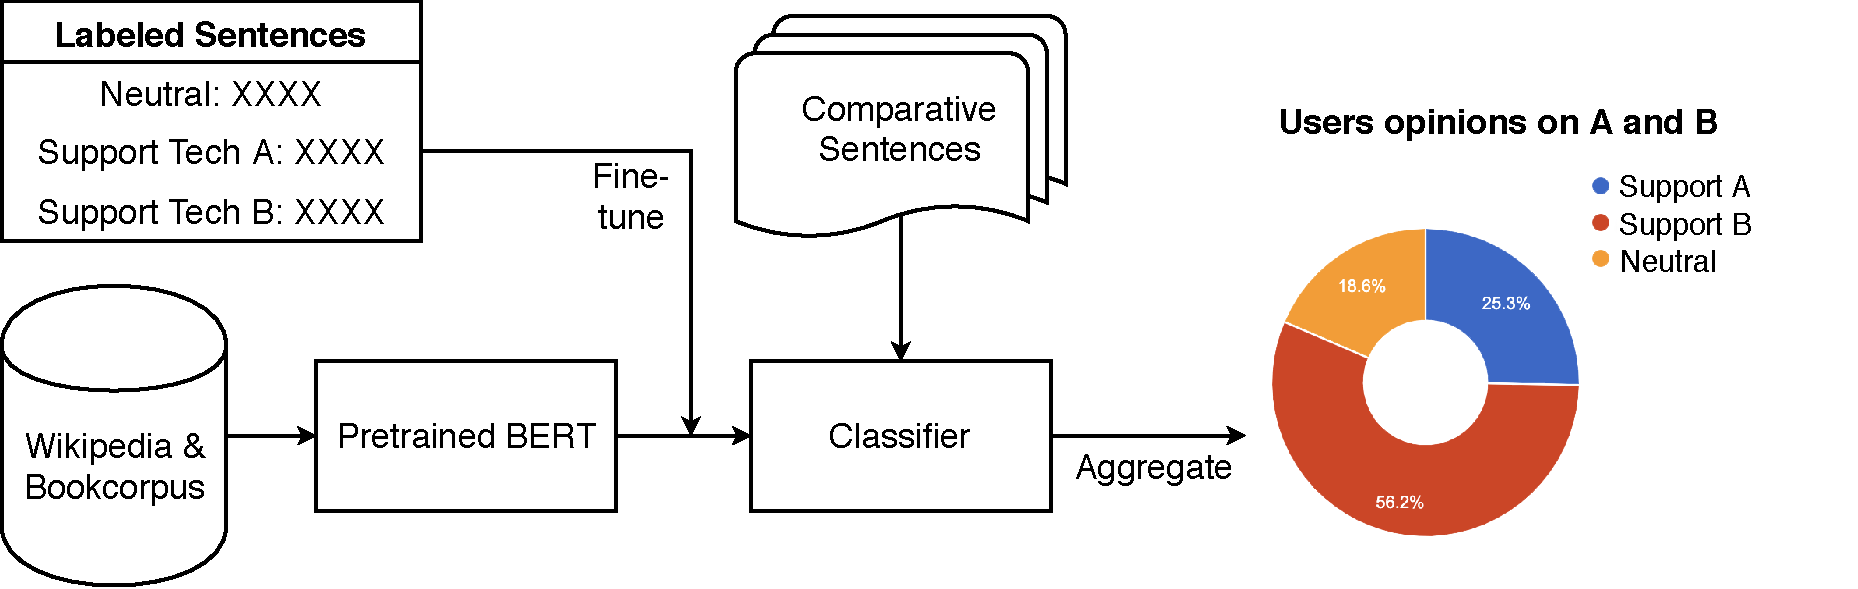
\includegraphics[width=0.45\textwidth]{figures/bert.pdf}
	\vspace{-2mm}
	\caption{\revise{Summerizing overall opinions towards each technology}}
	\label{fig:finetune}
\end{figure} 
\revise{For some comparable technologies, there may be too many comparison opinions which are too time-consuming for developers to read all of them.
Therefore, we further develop a sentiment classifier based on the BERT model~\cite{devlin2018bert} for automatically distilling the overall opinion towards the comparable technologies.
That summarization can be an important criteria for developers to determine which technology to adopt.}
\chen{Please draw a flow chart for this process including: 1) preprocessing the data, labeling data, splitting data 2) introduce the pretrained BERT model 3) fine tune the model 4) get the summarization sentiment.}\wang{The general process of summarising overall opinion is shown in Fig.~\ref{fig:finetune}}

\begin{comment}
While comparing two techniques, users also would like to see an overall opinion on which technology is better or which one should they use.  
After collecting all the comparative sentences, we randomly picked several sentences and label them based on semantically which technology they think is better. After that, we use BERT\cite{devlin2018bert} model to train the labeled sentences, and manage to predict which technology the writer suggest from the comparative sentences. For each comparable technology pair, we collect all the prediction of sentences and generate an overall opinion for each pair.
\end{comment}

\begin{figure*}
	\centering
	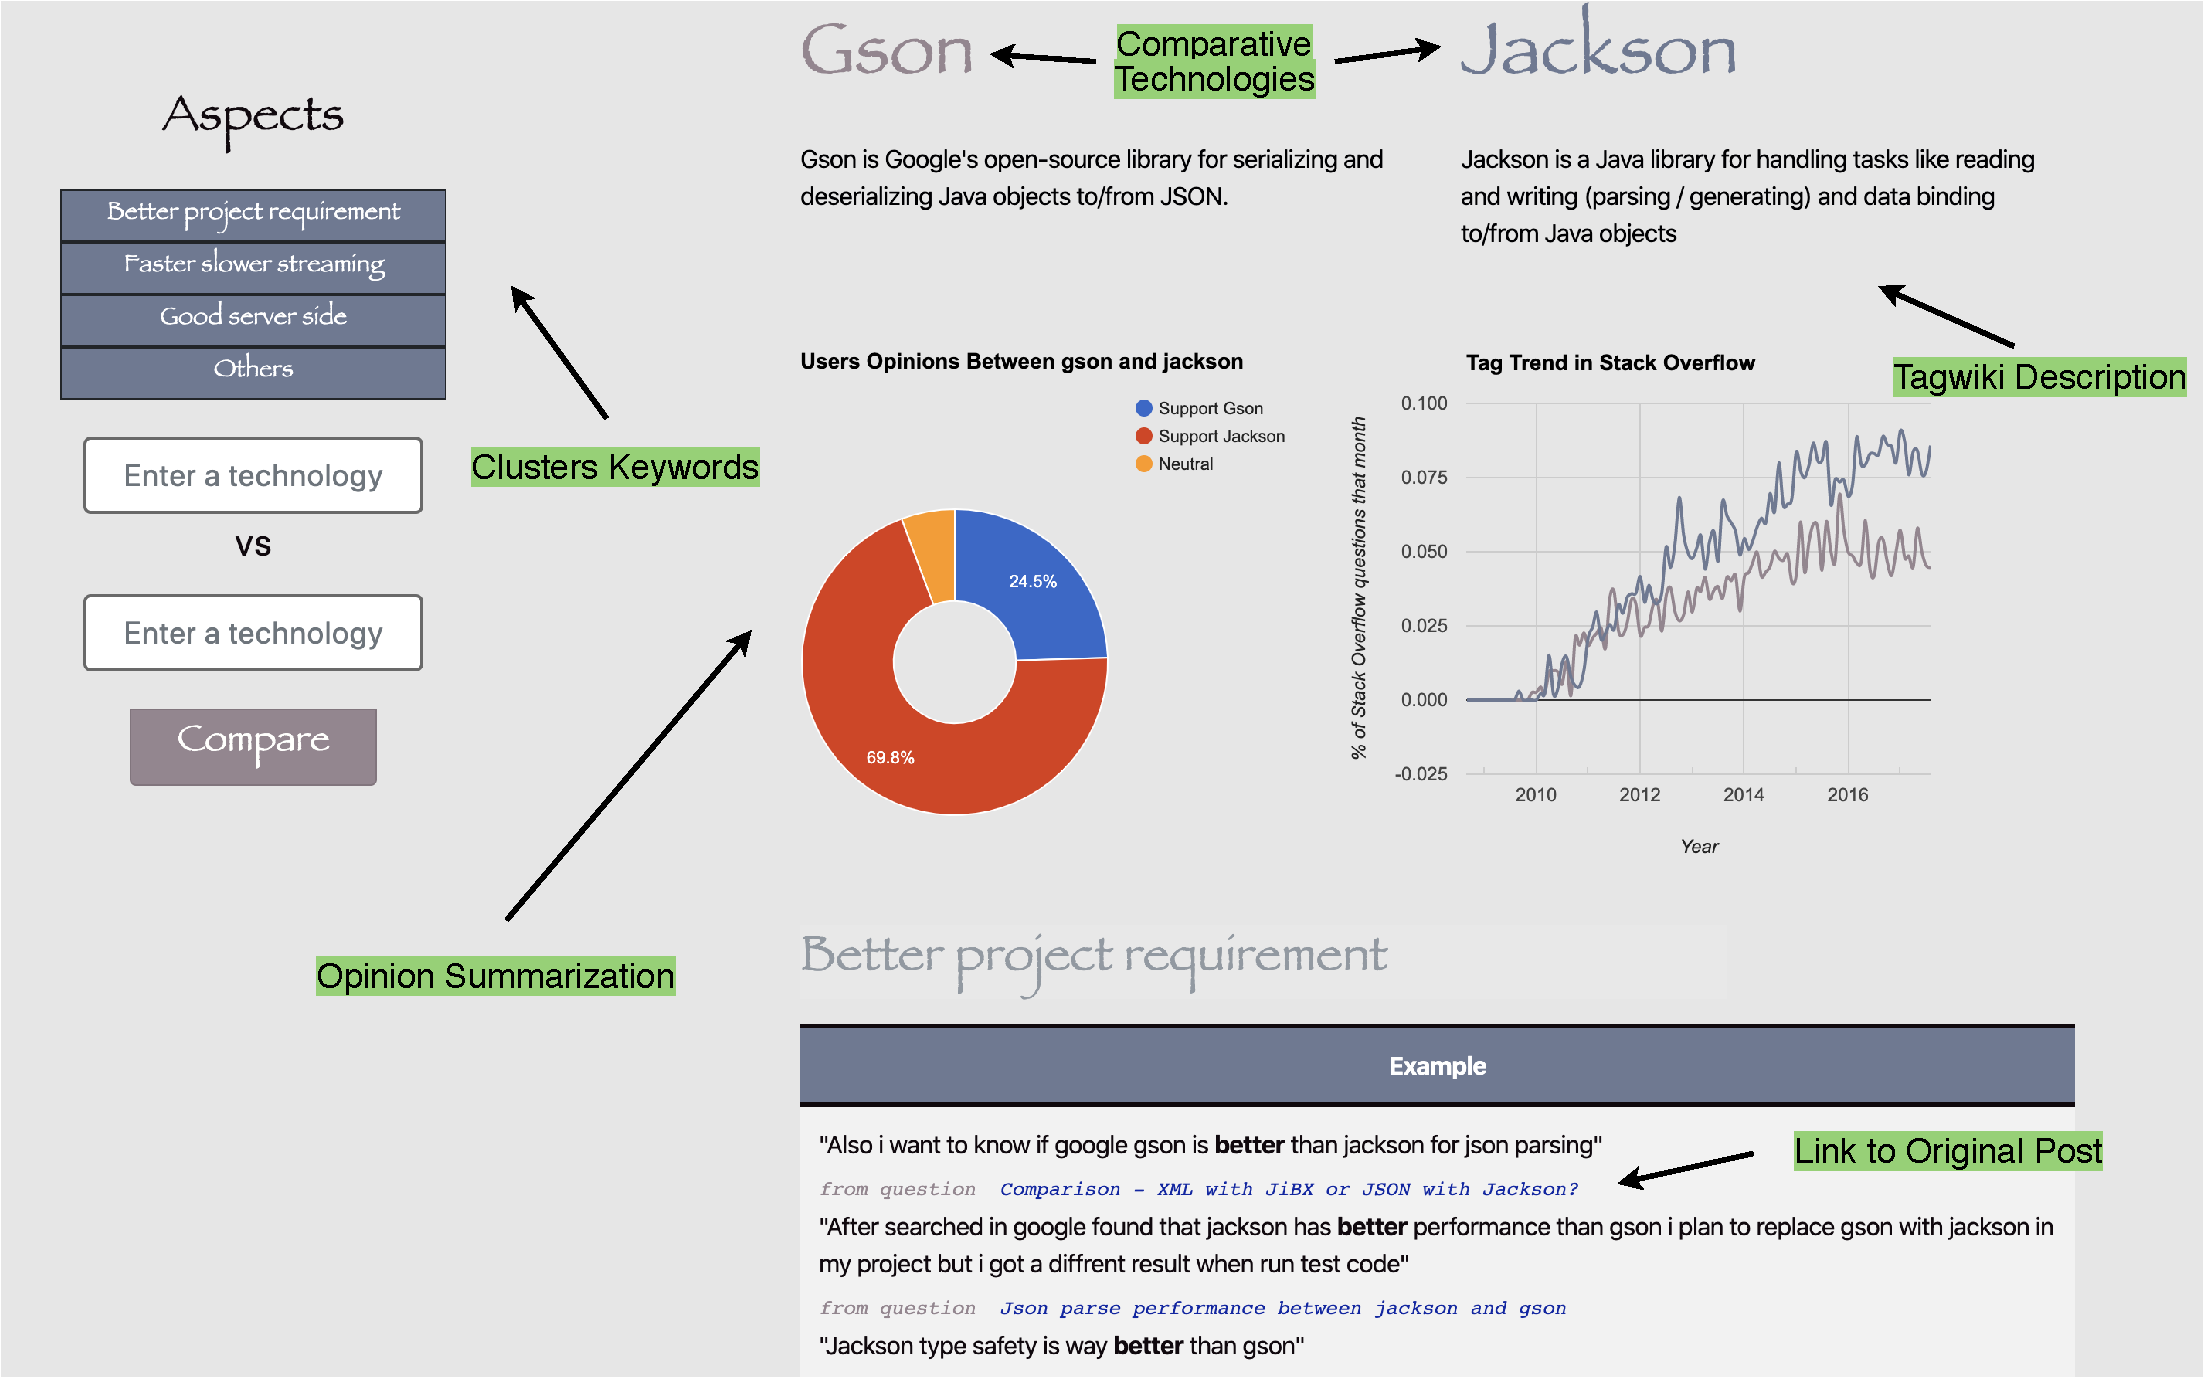
\includegraphics[height=90mm]{figures/website.pdf}
	\vspace{-3mm}
	\caption{The screenshot of our website \textit{DiffTech} and some important elements in the website \chen{1) The first sentence is a question actually that should be removed; 2) Can we find change another example that there is no explicit comparison posts? 3) For the webpage, can we add a line after the tagwiki, and a line after the trend? 4) For the trend graph, how to know which line is for which technology? 5) The clustering of this example is not good, so change another example.}}
	\vspace{-3mm}
	\label{fig:website}
\end{figure*} 

\revise{
For summarizing the overall opinions toward comparable technologies, we formulate it as a classification problem.
Given a set of comparative sentences about them, we build a classifier for identifying which technology does each sentence support.
By counting the total number of support sentences for each technology, we obtain the sentiment summarization of them.
We replace the comparable technology pairs with two unique tokens i.e., TechA (first occurrence) and TechB (second occurrence) to generalize different technology pairs.
We randomly select 801 comparative sentences and replace the comparable technology pairs with two unique tokens i.e., TechA (first occurrence) and TechB (second occurrence) to generalize different technology pairs.}

\begin{comment}
As mentioned above, we use BERT, which stands for Bidirectional Encoder Representations from
Transformers, for deploying sentence analysis. There are already plenty of pre-trained models in the market, we choose BERT because it supposed to be the first deeply bidirectional, unsupervised language representation, pre-trained using only a plain text corpus\cite{web:bertblog}. And quite a lot works have proved that BERT model \wang{find some reference} has surpassed other  transformers.
\end{comment}

\begin{figure}
	\centering
	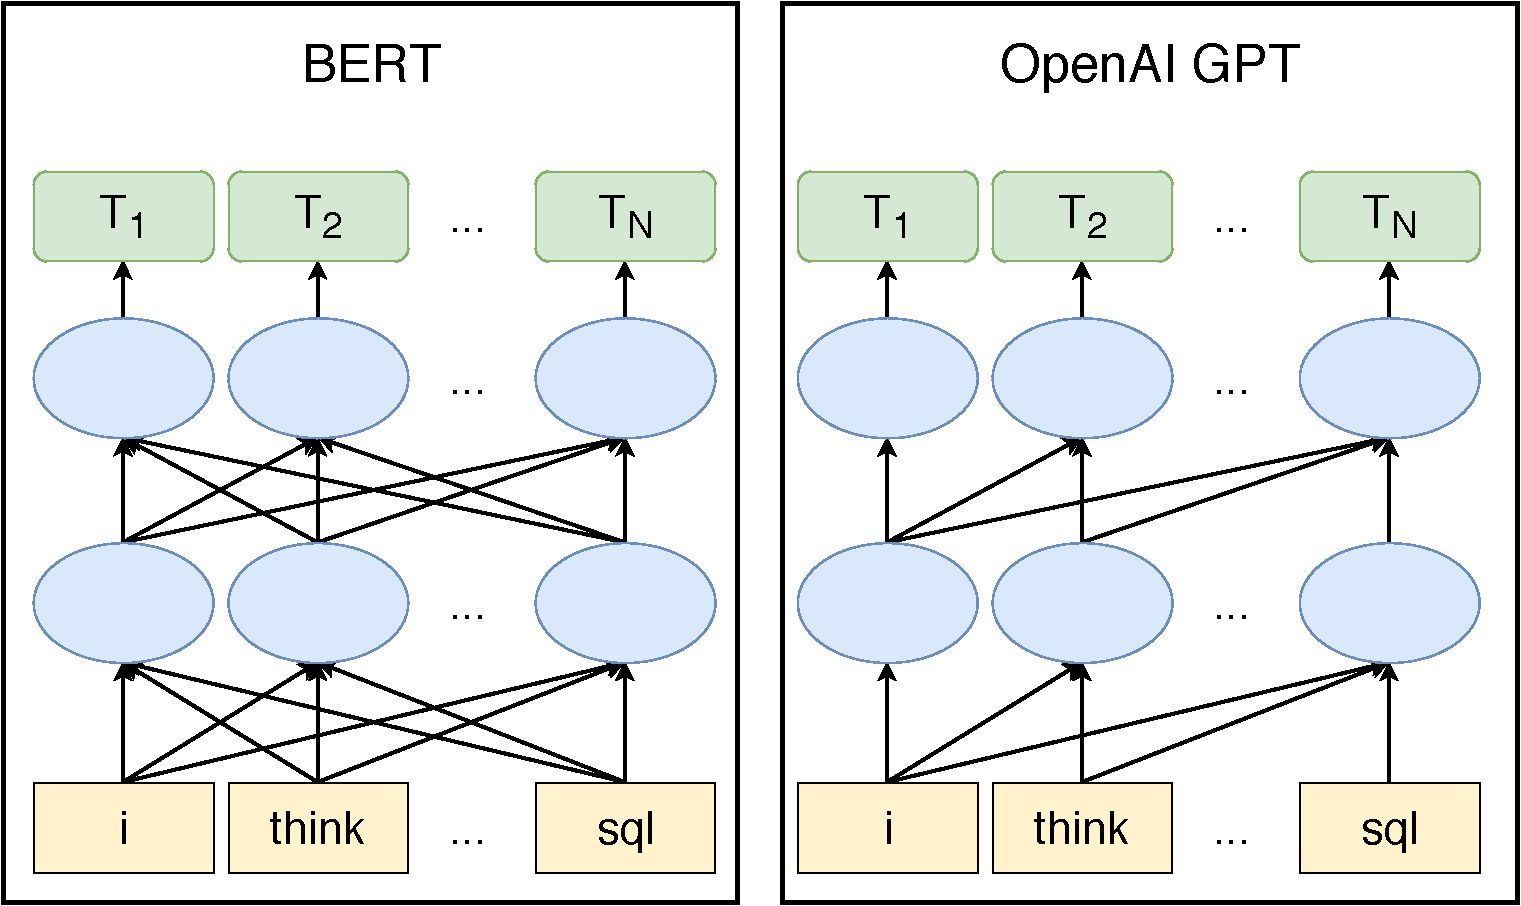
\includegraphics[height=50mm]{figures/bertmodel.pdf}
	\vspace{-3mm}
	\caption{BERT deeply bidirectional architecture compare with OpenAI GPT which is unidirectional}
	\vspace{-3mm}
	\label{fig:bertmodel}
\end{figure}
%\subsection{Constructing the classifier}
%\label{sec:fineTuning}
\revise{
However, the supervised learn requires a large-scale labeled dataset which labour-extensive and time-consuming.
To overcome this issue, we adopt the state-of-the-art model, BERT for this work.
BERT (Bidirectional Encoder Representations)~\cite{devlin2018bert} is \wang{the first deeply bidirectional unsupervised language representation, pre-trained using only a plain text corpus\cite{web:bertblog}. Fig~\ref{fig:bertmodel} shows its architecture compare with a unidrectional representation. For each word, BERT considers its different meanings in different contextual environments. For example, the word `chair' would have same representation in `seat a the chair' and `the chair of the committee' for a context-free models. A contextual model like BERT would have one representation of each word that is based on the other words in its surroundings.  BERT also introduce the ``masked language modeling'', which is to make sure BERT is a deep bidirectional representation. While doing the training, the model will randomly mask some percentage of the input tokens, and predict them. For example, the \textbf{Input} is ``A Lady went to the [MASK1]. She bought a [MASK2] of pork belly.'' and the \textbf{Labels} are ``MASK1=butcher,MASK2=tray''. Those features make BERT different but powerful than other pre-trained representations. }
In addition, Google release a pretrained BERT model~\cite{web:bertmodel} based on the large-scale corpus including Wikipedia and BookCorpus~\cite{moviebook} which contains 2,500 million words from English wikipedia sentences and 800 million words from 11,038 unpublished books.
As the pretrained model is well trained based on such big data and long time, it already encodes a lot of information about our general language. 
To leverage that learned knowledge, we only fine tune the pretrained BERT model by adding a new layer on the top of it.
We freeze the parameters of existing pretrained model but only train the final layer based on a small manually-labeled dataset for adapting it with domain-specific information.
}

\begin{comment}
BERT has already been trained with large amount of plain text, so we only need to provide a small set of data to BERT for fine-tune. And expect it the model to return its predictions. 
From all the comparative sentences, we randomly select around 800 sentences as training corpus. We firstly replace the comparable technology pairs with two unique tokens e.g. Tech A and Tech B, to reduce the ambiguity of different technology pairs.  For each sentence, we have three possible labels as 0, 1, 2. A sentence will be labeled as 0 if itself is neutral and we can't see which technology is better. Label 1 means that we can predict that tech A is better than tech B on some certain aspect or overall speaking, whereas label 2 means the opposite. Table~\ref{tab:label} shows some sample sentences we labeled and all the labeled sentences construct the training corpus for fine-tuning.
\end{comment}



\begin{comment}
Then, we further process the sentences to structures that BERT can understand. The process start with breaking sentences into tokens and add start mark "CLS" and end mark "SEP"to all tokenized sentences. We also add the index and segment id from words in sentences to the input data based on the provided BERT vocabulary file.

We use the TensorFlow estimator to train and predict data. After preprocing the data input, we load the BERT model and create a new layer on the top of it. The new layer then get trained, and after a few epoch of training, the new model will be able to predict sentences based on the training samples.

\end{comment}



\section{Implementation}
\begin{figure}%
\centering
\subfigure[Visiting Statistics]{%
\label{fig:stats}%
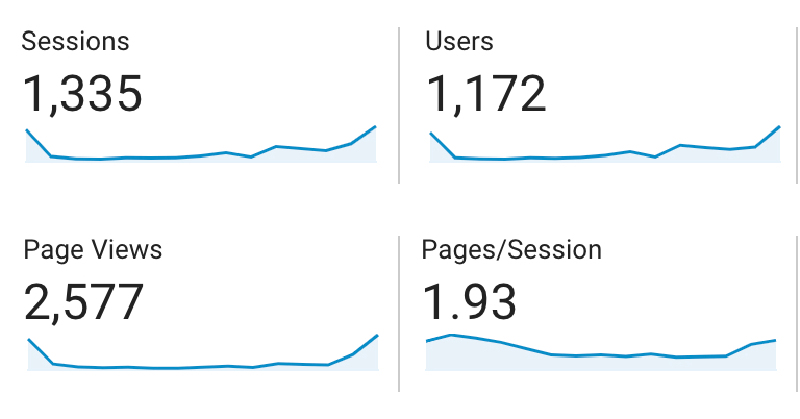
\includegraphics[width=0.23\textwidth]{figures/stats.pdf}}%
\qquad
\subfigure[Returning Users]{%
\label{fig:return}%
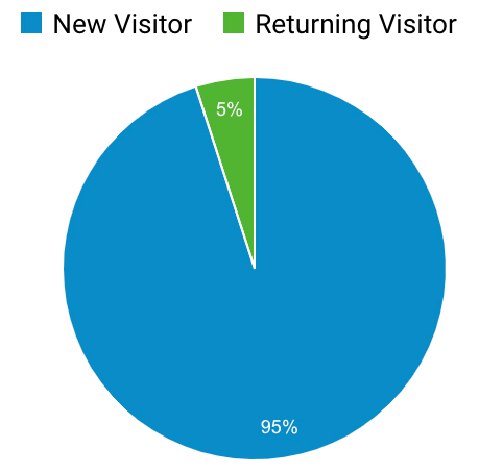
\includegraphics[width=0.17\textwidth]{figures/returning.pdf}}%
\qquad
\subfigure[Geo Map]{%
\label{fig:map}%
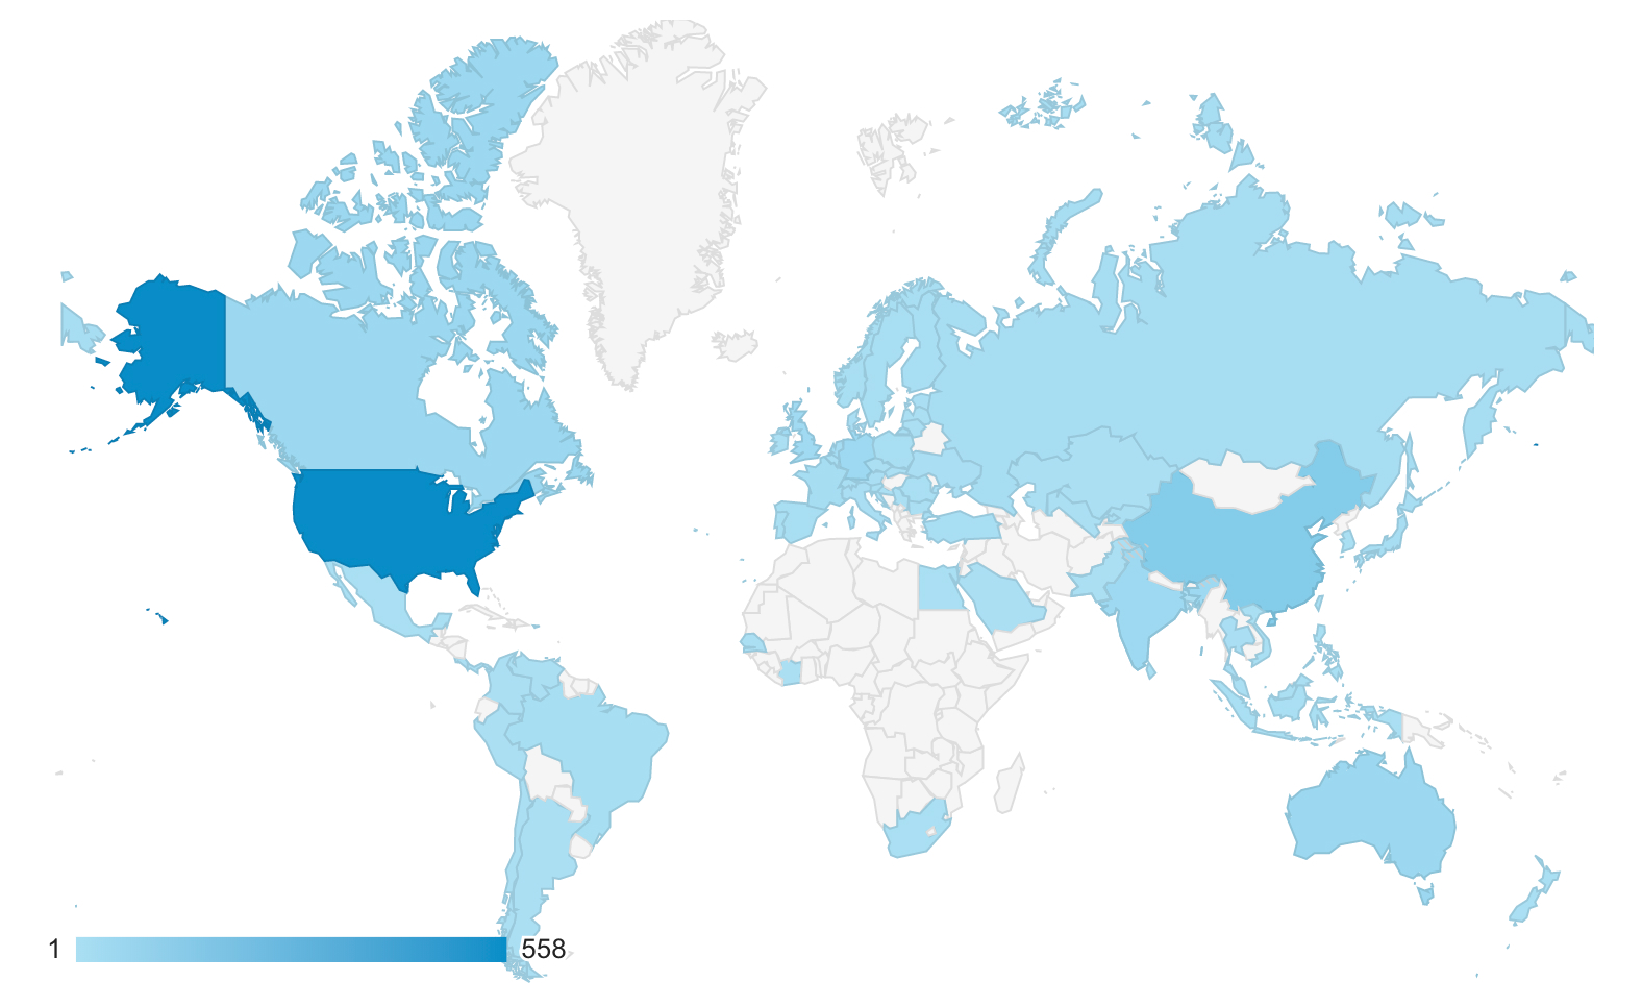
\includegraphics[width=0.4\textwidth]{figures/theworld.pdf}}%

\caption{The traffic of our website from Google Analytics\chen{This is too large, make it to a single-column figure with (a) and (c) in the first row while the map in the second row.}}
\label{fig:googleanalytics}
\end{figure}

\subsection{Dataset}
We take the latest Stack Overflow data dump (released on 4 September 2019) as the data source.
It contains 18,154,493 questions with 55,665 unique tags, and 27,765,324 answers.
With the approach in Section~\ref{sec:similarTech}, we collect in total 14,876 pairs of comparable technologies.
Among these technologies, we extract 19,118 comparative sentences for 2,410 pairs of comparable technologies.
We use these technology pairs and comparative sentences to build a knowledge base for technology comparison.

\subsection{Tool Support}
Based on the our proposed approach, we implement a practical website\footnote{\url{https://difftech.herokuapp.com/}} for developers.
With the knowledge base of comparable technologies and their comparative sentences mined from Stack Overflow, our site can return an informative and aggregated view of comparative sentences in different comparison aspects for comparable technology queries.
In addition, the tool provides the link of each comparative sentence to its corresponding Stack Overflow post so that users can easily find more detailed content. 
\wang{For example, as shown in Fig~\ref{fig:website}, given a pair of comparable technologies \textit{Gson} and \textit{Jackson}, the definition of them from TagWiki is below each technology name. 
About 69.8\% of the users support using \textit{Jackson} instead of \textit{Gson}. 
The post trend shows that \chen{although both technologies are more and more popular, there are more discussion about Jackson.}
We could also see that the method clustered all the comparative sentences into four clusters and has been clarified at the top left corner. 
For each clustered aspect, we list the comparative sentences below and attach the direct link for each comparative sentence to its original post.
User can click the link for retrieving more content.}

\subsection{Visitor Analysis}
\wang{We initially released our website on September 2018, and has updated data and layout on September 2019. We posted the news on some websites such as StackApps~\cite{??} and Reddit~\cite{??} as well for propaganda purpose. } 
\chen{You may update the following part if you have more data.}
\revise{We embedded Google Analytics into our website to monitor the site traffic. 
Fig.~\ref{fig:googleanalytics} shows that about 1,200 users from 75 different countries visited our website. 
These users viewed 2,577 different pages and in average 1.93 pages for each session. 
Note that most users come to our site with very specific target, i.e., comparing a pair of similar technologies, so, the average number of visited pages in each session is rather small.
By tracking their IP, we find that most users come from the U.S. (47.6\%), and other countries such as China (10.8\%), Australia (4\%), Canada (4\%), etc. 
Nearly 5\% of the users come back to visit our website again, indicating the usefulness and attraction of our site.
%Both the data from Google Analytics and users' comments after using our website, shows their interests and needs to our methods in comparing technologies, especially for those who are new to this area. 
}

%\wang{We find that the average page number users view per session is a bit low. This might be ascribed to the page design. For those people visiting the home page, if they can't find the desired technologies underneath, they might try to use search bar. However, it seems not clear for them to search which comparative technology pairs are available in our website. Then, for users who already is in the compare page, they might find themselves interested in certain answer ,click the question link, and end up with leaving our site to StackOverflow. }

\revise{
Among all visiting technology pairs, users compared \textit{Mysql} with \textit{Postgresql} most frequently (197 times) and other frequent technology pairs like \textit{tco vs udp}, \textit{lisp vs scheme}.
Apart from the visiting, some users also post comments under our advertisements in Reddit such as  ``\textit{Thank you ...will share the word}'', ``\textit{It was actually better than I expected, at least for the suggested comparisons. Good job!}''.
They also provide some constructive suggestion for improving our tool like \chen{``\textit{This sounds interesting. However I think it would be better if there were options to add to the technologies, pros, cons and usage.}''}, and we will further add more features in our site to make it more powerful. 
%and some suggestions on further category pros and cons for each technology. 
%In general, our website  fulfill our intention to build the site, which is to provide a platform for developers to compare similar technologies, aggregate opinions, and give suggestions. 
}





\begin{figure}
	\centering
	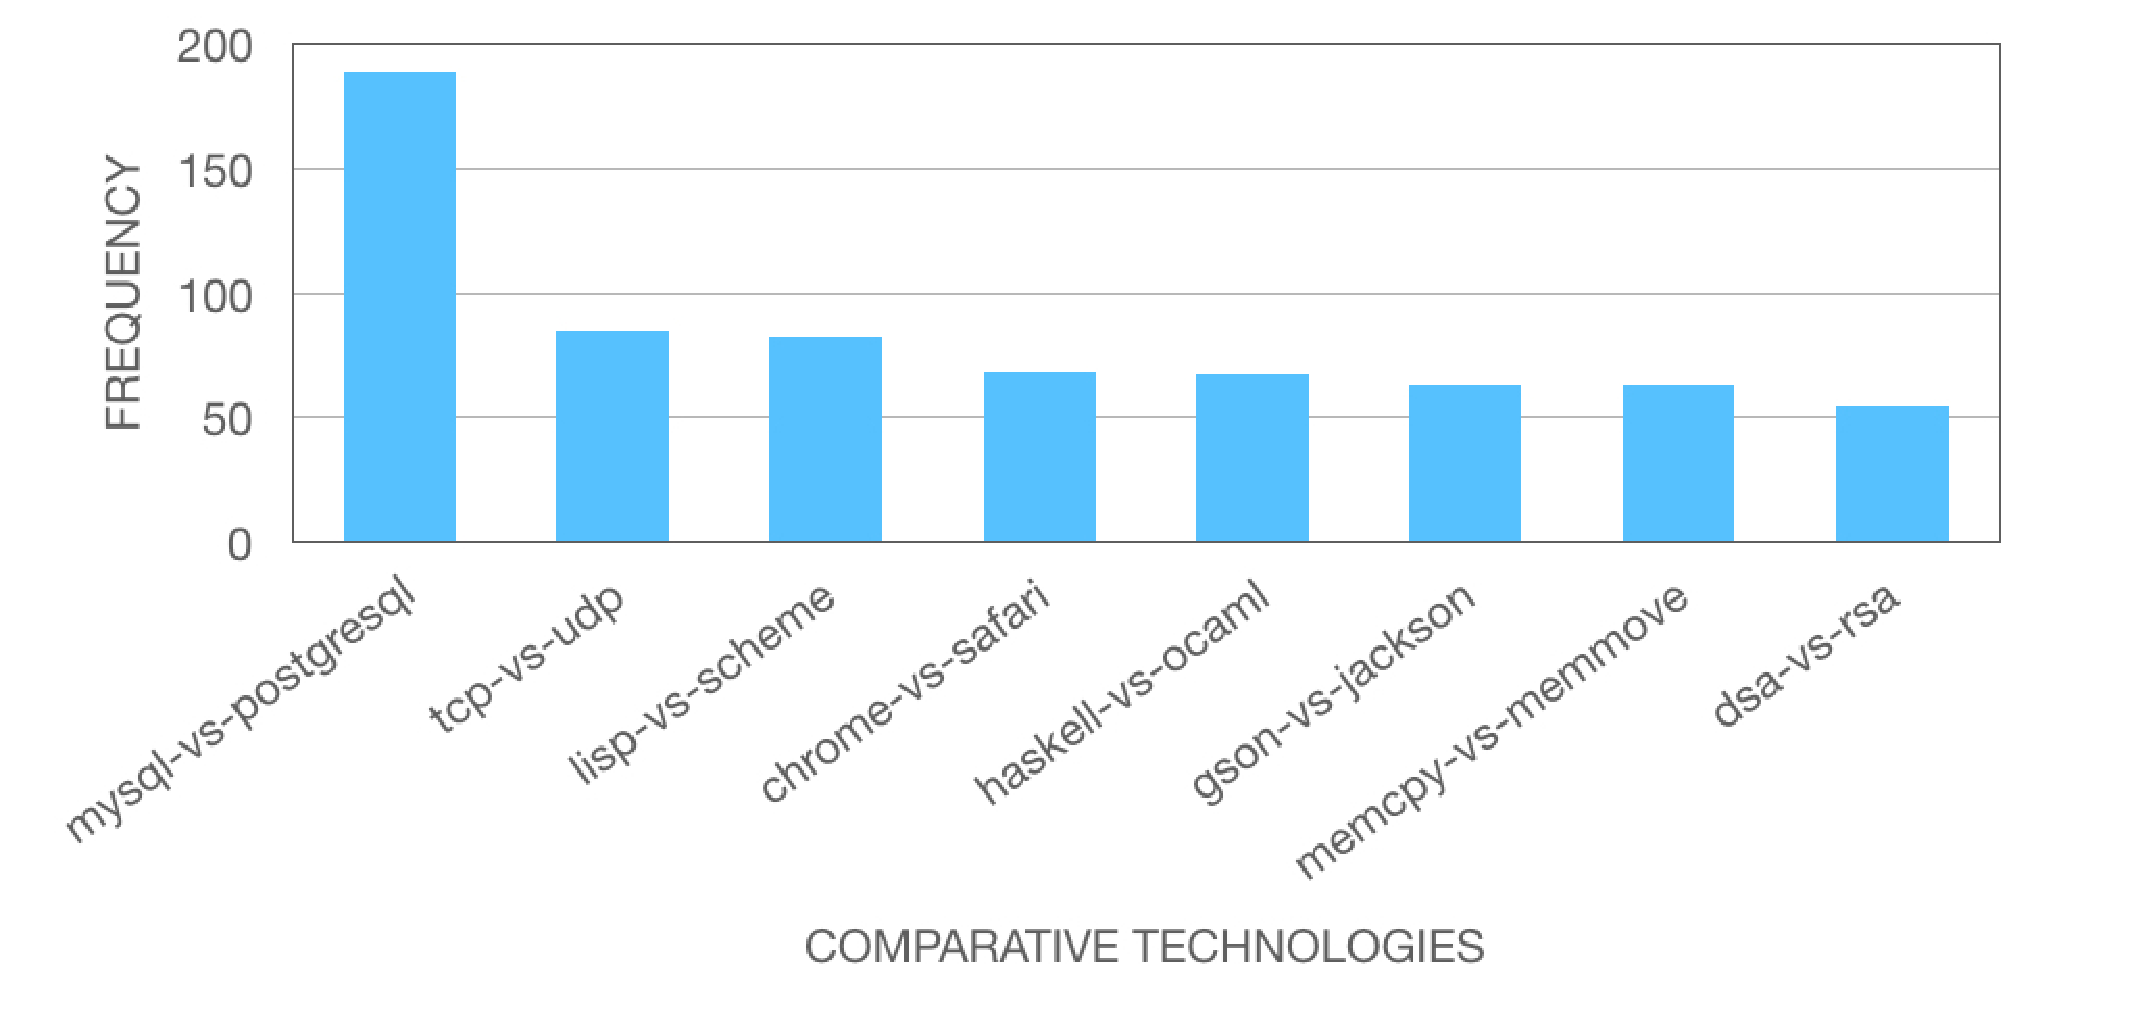
\includegraphics[width=0.49\textwidth]{figures/barChart.pdf}
	\vspace{-3mm}
	\caption{Top 8 most visited pages \chen{1)Make the labels larger 2)make it more flat for taking less vertical space.}}
	\vspace{-3mm}
	\label{fig:barChart}
\end{figure} 

\section{Experiment}
\label{sec:experiment}
In this section, we evaluate each step of our approach.
As there is no ground truth for technology comparison, we have to manually check the results of each step or build the ground truth.
And as it is clear to judge whether a tag is of a certain category from its tag description, whether two technologies are comparable, and whether a sentence is a comparative sentence, we recruit two Master students to manually check the results of these three steps.
Only results that they both agree will be regarded as ground truth for computing relevant accuracy metrics, and those results without consensus will be given to the third judge who is a PhD student with more experience.
All three students are majoring in computer science and computer engineering in our school, and they have diverse research and engineering background with different software tools and programming languages in their work.
In addition, we release all experiment data and results in our website\footnote{\url{https://sites.google.com/view/difftech/}}.
 

\subsection{Accuracy of Extracting Comparable Technologies}
This section reports our evaluation of the accuracy of tag category identification, the important of tag category for filtering out irrelevant technologies, and the impact of word embedding models and hyperparameters.

\subsubsection{The Accuracy of Tag Category}
From 33,306 tags with tag category extracted by our method, we randomly sample 1000 tags whose categories are determined using the NLP method, and the other 1000 tags whose categories are determined by the dictionary look-up method (see Section~\ref{sec:categoryKG}).
%As it is clear that whether a tag represents a programming language, a library, or a general computing concept and whether the extracted category corresponds to what a tag represents, 1 final-year Computer Science undergraduate students are recruited to manually examine the category of these 2000 tags by reading their corresponding TagWiki.
%we assign different participants with different sets of tags, so that we can examine as many results as possible with limited number of participants. 
%In this experiment, each participant is assigned 200 tags from the NLP method, and 200 tags from the dictionary look-up method for checking.
Among the 1000 sampled tag categories by the NLP method, categories of 838 (83.8\%) tags are correctly extracted by the proposed method.
For the 1000 sampled tags by the dictionary look-up method, categories of 788 (78.8\%) tags are correct.

According to our observation, two reasons lead to the erroneous tag categories.
First, some tag definition sentences are complex which can lead to erroneous POS tagging results.
For example, the tagWiki of the tag \textit{rpy2} states that ``RPy is a very simple, yet robust, Python interface to the R Programming Language''. 
The default POS tagging	recognizes \textit{simple} as the noun which is then regarded as the category by our method.
Second, the dictionary look-up method sometimes makes mistakes, as the matched category may not be the real category.
For example, the TagWiki of the tag \textit{honeypot} states ``A trap set to detect or deflect attempts to hack a site or system''.
Our approach matches the \textit{system} as the category of the \textit{honeypot}.

\subsubsection{The Importance of Tag Category}
To check the importance of tag category for the accurate comparable technology extraction, we set up two methods, i.e., one is word embedding and tag category filtering, and the other is only with word embedding.
The word embedding model in two methods are both skip-gram model with the word embedding dimension as 800.  
We randomly sample 150 technologies pairs extracted from each method, and manually check the if the extracted technology pair is comparable or not.
It shows that the performance of model with tag category (90.7\%) is much better than that without the tag category filtering (29.3\%).

\subsubsection{The impact of parameters of word embedding}
%The are two kinds of widely-used word embedding models, the skip-gram model and CBOW model mentioned in Section~\ref{sec:w2v}.
\label{sec:comparison_w2v}
There are two important parameters for the word embedding model, and we test its impact on the the performance of our method.
First, we compare the performance of CBOW and Skip-gram mentioned in Section~\ref{sec:w2v} by randomly sampling 150 technology pairs extracted by each method under the same parameter setting (the word embedding dimension is 400).
The results show that Skip-gram model (90.7\%) outperforms the CBOW model (88.7\%), but the difference is marginal.

Second, we randomly sample 150 technologies pairs by the skip-gram model with different word embedding dimensions, and manually check the accuracy.
From the dimension 200 to 1000 with the step as 200, the accuracy is 70.7\%, 72.7\%, 81.3\%, 90.7\%, 87.3\%.
We can see that the model with the word embedding dimension as 800 achieves the best performance.
Finally, we take the Skip-gram model with 800 word-embedding dimension as the word embedding model to obtain the comparable technologies in this work.   

\subsection{Accuracy and coverage of comparative sentences}
We evaluate the accuracy and coverage of our approach in finding comparative sentences from the corpus.
\wang{We first randomly sample 350 sentences (50 sentences for each comparative sentence pattern in Table~\ref{tab:patternSingle} and Table~\ref{tab:patternMultiple}) which are extracted by our model.
We manually check the accuracy of the sampled sentences and Table~\ref{tab:patternAccuracy} shows the results.
The overall accuracy of comparative sentence extraction is 89.1\%, and our approach is especially accurate for the first 2 patterns for single sentence and all three patterns for contextual sentences.
The last two patterns for single sentence do not get good performance due to the relatively loose conditions.}

\wang{
We further check the wrong extraction of comparative sentences and find that most errors from single sentence patterns are caused when the two comparative technologies are listed together for a similar feature, i.e. ``\textit{Java framework awt or swing makes more sense for something this simple}''} or when the two comparative technologies are used to compare with a third technology like ``\textit{I mean it came as a surprise to me that drupal is so much faster than wordpress and joomla}''.
In addition, although some sentences do not contain the question mark, they are actually interrogative sentence such as ``\textit{I also wonder if postgresql will be a win over mysql}''.
\wang{
For contextual sentences, we also find out that sometimes the sentence is comparing the two selected technology pairs with a third one. And sometimes for the AFF-NEG pattern, it seems although both sentences mentioned two comparative technologies respectively, they aren't tended to compare them, i.e. ``\textit{Vim does only text editing and that very well without plugins.
Its up to you if you like emacs or not.}''}
%Second, the comparison between the two similar technologies is quantitive (e.g., a \textit{ng-app} can have more than one \textit{ng-controller}).

\begin{comment}
\begin{figure}
	\centering
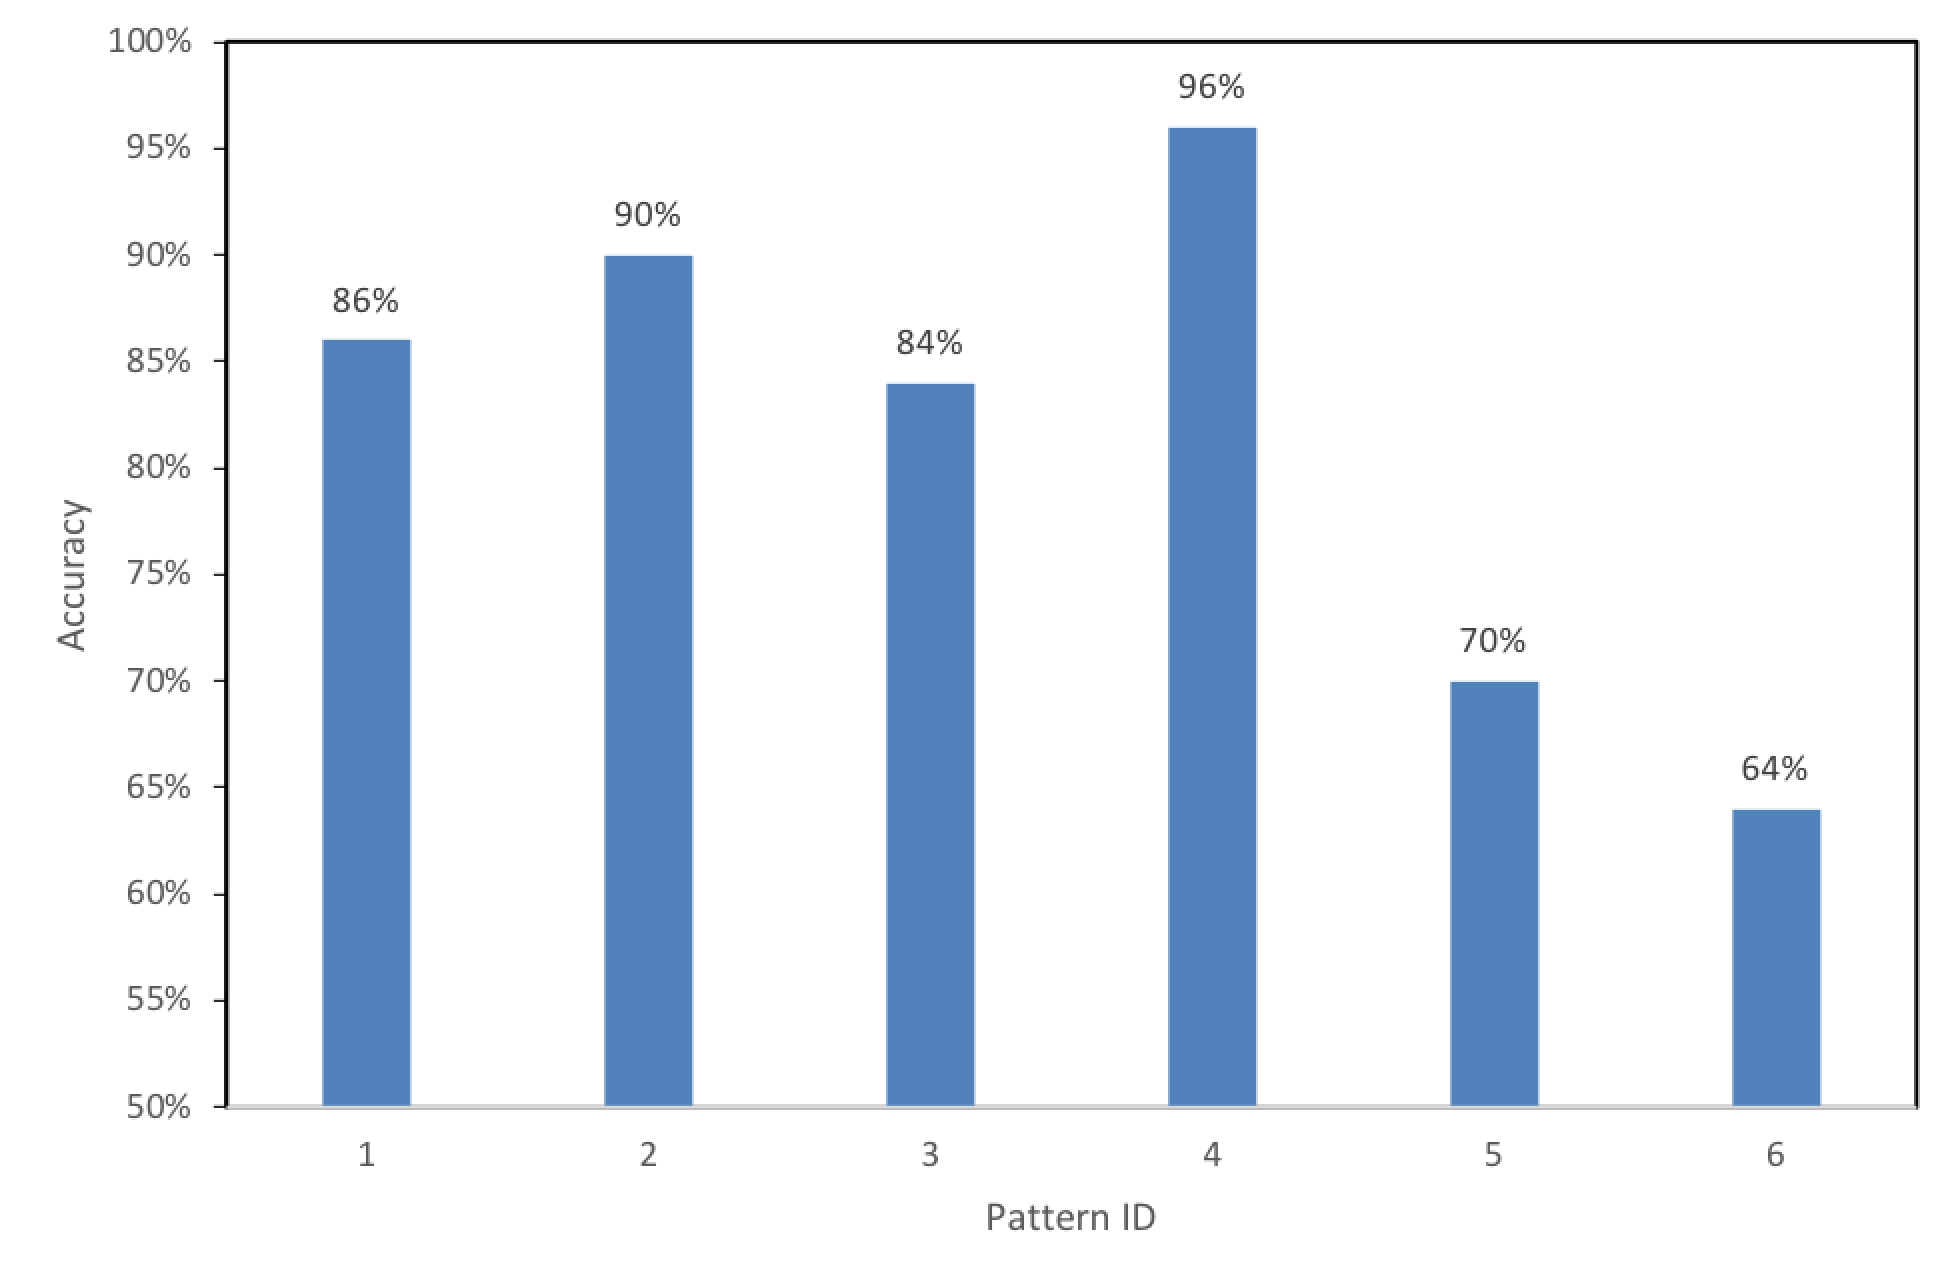
\includegraphics[width=0.5\textwidth]{figures/patternAccuracy.png}
	\label{fig:patternAccuracy}
\end{figure}	
\end{comment}


\begin{table}
	\centering
	\caption{The accuracy of comparative sentences extraction}
	\vspace{-2mm}
	\begin{tabular}{c c c c c}
	\hline
	\multicolumn{5}{c}{Single sentence}\\
	\hline
	\textbf{No.} & Pattern & \textbf{\#right} & \textbf{\#wrong} & \textbf{Accuracy} \\ \hline
	1 & \textit{TECH * VBZ * JJR/RBR} & 47 & 3  & 94\% \\
	2 & \textit{(RBR JJ) /JJR * CIN * TECH} & 46 & 4  & 92\% \\
	3 & \textit{CV * CIN TECH} & 42 & 8 & 82\% \\
	4 & \textit{CV VBG TECH} & 38 & 12 & 76\% \\
	\hline
	\multicolumn{5}{c}{Contextual sentences}\\
	\hline
	\textbf{No.} & Pattern & \textbf{\#right} & \textbf{\#wrong} & \textbf{Accuracy} \\ \hline
	1 & \textit{TECH * VBZ * JJR/RBR} & 47 & 3  & 94\% \\
	2 & \textit{(RBR JJ) /JJR * CIN * TECH} & 47 & 3  & 94\% \\
	3 & \textit{AFF-NEG} & 45 & 5  & 90\% \\
	\hline
	Total &  & 312 & 38 & 89.1\% \\
	\hline
	\end{tabular}
	\vspace{-2mm}
	\label{tab:patternAccuracy}
\end{table}

\begin{comment}
To measure the coverage, we first find all sentences that contain pairs of similar technologies.
Then we randomly sample 200 sentences of them, and find \textcolor{red}{??} sentences are comparative sentences via the manual check.
Among \textcolor{red}{??} comparative sentences, \textcolor{red}{?? (??\%) of them are successfully extracted by our approach.}
\textcolor{red}{For the ?? comparative sentences we missed, we conclude xx reasons: 1) 2) CCY: Please tell why we cannot find some of them.}
%For coverage, we compare the baseline without using synonyms and abbreviations in our previous work~\cite{chen2017unsupervised}.
\end{comment}

\subsection{Accuracy of clustering comparative sentences}
\label{sec:clusterEvaluate}
We evaluate the performance of our opinion clustering method by comparing it with the baseline methods.

\subsubsection{Baseline}
\wang{
We set up three baselines to compare with our comparative sentence clustering method. 
The first baseline is the traditional TF-IDF~\cite{sparck1972statistical} with K-means~\cite{hartigan1979algorithm}, the second baseline is based on the document-to-vector deep learning model (i.e., Doc2vec~\cite{le2014distributed}) with K-means, and the last one is BERT~\cite{devlin2018bert} with K-means.
All of methods first convert the comparative sentences for a pair of comparable technologies into a list of vectors.
%We train both models with all comparative sentences in our corpus.
Then, we carry out K-means algorithms to cluster the sentence vectors into $N$ clusters.
To make the baseline as competitive as possible, we set $N$ at the cluster number of the ground truth.
In contrast, our method specifies its cluster number by community detection which may differ from the cluster number of the ground truth.}
\chen{Will check this paragraph later.}

\subsubsection{Ground Truth}
\label{sec:clusteringGroundTruth}
As there is no ground truth for clustering comparative sentences, we ask two Master students mentioned before to manually build a small-scale ground truth.
We randomly sample 15 pairs of comparable technologies with different number of comparative sentences.
For each technology pair, the two students read each comparative sentence and each of them will individually create several clusters for these comparative sentences.
Note some comparative sentences are unique without any similar comparative sentence, and we put all those sentences into one cluster.
Then they will discuss with the Ph.D student about the clustering results, and change the clusters accordingly.
Finally, they reach an agreement for 10 pairs of comparable technologies.
We take these 10 pairs as the ground truth whose details can be seen in Table~\ref{tab:groundTruth}.

\begin{table}
	\centering
	\small
	\caption{Ground truth for evaluating clustering results}
	\vspace{-2mm}
	\setlength{\tabcolsep}{0.01em}
	\begin{tabular}{c c c c}
	\hline
	\textbf{No.} & \textbf{Technology pair} & \textbf{\#comparative sentence} & \textbf{\#cluster} \\ \hline
	1 & \textit{compiled \& interpreted language} & 34 & 4 \\
    2 & \textit{sortedlist \& sorteddictionary} & 18 & 4 \\
	3 & \textit{quicksort \& heapsort} & 51 & 5 \\
	4 & \textit{ant \& maven} & 83 & 9 \\
	5 & \textit{lxml \& beautifulsoup} & 52 & 6 \\
	6 & \textit{awt \& swing} & 53 & 7 \\
	7 & \textit{jackson \& gson} & 39 & 3 \\
	8 & \textit{jruby \& mri} & 25 & 4 \\
	9 & \textit{pypy \& cpython} & 72 & 7 \\
	10 & \textit{memmove \& memcpy} & 33 & 3 \\
	\hline
	\end{tabular}
	\vspace{-3mm}
	\label{tab:groundTruth}
\end{table}

\subsubsection{Evaluation Metrics}
\label{sec:clusteringGroundTruth}
Given the ground truth clusters, many metrics have been proposed to evaluate the clustering performance in the literature.
In this work, we take the Adjusted Rand Index (ARI)~\cite{hubert1985comparing}, Normalized Mutual Information(NMI)~\cite{vinh2010information}, homogeneity, completeness, V-measure~\cite{rosenberg2007v}, and Fowlkes-Mallows Index (FMI)~\cite{fowlkes1983method}.
For all six metrics, higher value represents better clustering performance.
For each pair of comparable technologies, we take all comparative sentences as a fixed list, and $G$ as a ground truth cluster assignment and $C$ as the algorithm clustering assignment.

\textbf{Adjusted Rand Index (ARI)} measures the similarity between
two partitions in a statistical way.
It first calculates the raw Rand Index (RI) by $ RI = \frac{a+b}{C^{N}_{2}}$ where $a$ is the number of pairs of elements that are in the same cluster in $G$ and also in the same cluster in $C$, and $b$ is the number of pairs of elements that are in different clusters in $G$ and also in different clusters in $C$.
$C^{N}_{2}$is the total number of possible pairs in the dataset (without ordering) where $N$ is the number of comparative sentences.
To guarantee that random label assignments will get a value close to zero, ARI is defined as 
$$ ARI = \frac{RI - E[RI]}{\max (RI) - E[RI]}$$
where $E[RI]$ is the expected value of $RI$.

\textbf{Normalized Mutual Information (NMI)} measures the mutual information between the ground truth labels $G$ and the algorithm clustering labels $C$, followed by a normalization operation:
$$ NMI(G, C) = \frac{MI(G, C)}{\sqrt{H(G) H(C)}} $$
where $H(G)$ is the entropy of set $G$ i.e., $H(G) = - \sum^{|G|}_{i=1}P(i) \log (P(i)) $ and $P(i) = \frac{G_i}{N}$ is the probability than an objet picked at random falls into class $G_i$.
The $MI(G, C)$ is the mutual information between $G$ and $C$ where $MI(G, C) = \sum^{|G|}_{i=1} \sum^{|C|}_{j=1} P(i, j) \log ( \frac{P(i, j)}{P(i)P(j)} )$


\textbf{Homogeneity (HOM)} is the proportion of clusters containing only members of a single class by
$$ h = 1 - \frac{H(G|C)}{H(G)} $$
\textbf{Completeness (COM)} is the proportion of all members of a given class are assigned to the same cluster by
$$ c = 1 - \frac{H(C|G)}{H(C)} $$
where $H(G|C)$ is the conditional entropy of the ground-truth classes given the algorithm clustering assignments.

\textbf{V-measure (V-M)} is the harmonic mean of homogeneity and completeness
$$ v = 2 \times \frac{h\times c}{h+c} $$

\textbf{Fowlkes-Mallows Index (FMI)} is defined as the geometric mean of the pairwise precision and recall:
$$ FMI = \frac{TP}{\sqrt{(TP+FP)(TP+FN)}} $$
where $TP$ is the number of True Positive (i.e. the number of pairs of comparative sentences that belong to the same clusters in both the ground truth and the algorithm prediction), $FP$ is the number of False Positive (i.e. the number of pairs of comparative sentences that belong to the same clusters in the ground-truth labels but not in the algorithm prediction) and $FN$ is the number of False Negative (i.e the number of pairs of comparative sentences that belongs in the same clusters in the algorithm prediction but not in the ground truth labels).

\subsubsection{Overall Performance}
\wang{
Table~\ref{tab:clusterEvaluation} shows the evaluation results.
the three baseline methods has similar results whereas tf-idf and Sentence-Bert are slitly better, but our model significantly outperforms all models in all six metrics.}

According to our inspection of detailed results, we find two reasons why our model outperforms the baselines.
First, our model can capture the semantic meaning of comparative sentences.
TF-IDF can only find similar sentences using the same words but count similar words like ``secure'' and ``safe'' as unrelated.
While the sentence vector from Doc2vec is easily influenced by the noise as it takes all words in the sentence into consideration. \wang{The Bert model would break word that it doesn't recognised into pieces, i.e.heapsort to heap-, -sort. In this way they might conduct vectors that is not close to the original words. Also, the BERT model is trained by general corpus(like wikipeidia), which is different from our technology-specific dataset.}
Second, constructing the similar sentences as a graph in our model explicitly encodes the sentence relationships.
The community detection based on the graph can then easily put similar sentences into clusters.
In contrast, for the four baselines, the error brought from them is accumulated and amplified to K-means in the clustering phase.

\begin{table}
	\centering
	\caption{Clustering performance}
	\vspace{-2mm}
	\setlength{\tabcolsep}{0.5em}
	\begin{tabular}{lllllll}
	\hline
	\textbf{Method} & \textbf{ARI} & \textbf{NMI} & \textbf{HOM} & \textbf{COM} & \textbf{V-M} & \textbf{FMI} \\ \hline
	TF-IDF+Kmeans  & 0.09&0.24&0.35&0.28&0.26&0.25\\
	Doc2vec+Kmeans & 0.01&0.17&0.29&0.20&0.18&0.18\\
	%BERT+Kmeans & 0.01&0.18&0.31&0.20&0.19&0.18\\
	Bert+Kmeans & 0.10&0.24&0.35&0.28&0.26&0.26\\
	\tool & \textbf{0.65}&\textbf{0.67}&\textbf{0.76}&\textbf{0.77}&\textbf{0.72}&\textbf{0.71}\\
	\hline
	\end{tabular}
	\vspace{-1mm}
	\label{tab:clusterEvaluation}
\end{table}

\subsection{Accuracy of Opinion Summarization}
\label{sec:summarization}
\wang{All of this section are newly added}
\chen{Please add more details in this section}
In this section, we evaluate the accuracy of our overall opinion summarization. We compare our methods with five different baselines that are commonly used in sentence analysis. We implement those baselines and use four metrics to compare them with our methods, and our methods performs better in opinion summarization than the rest of them.

\subsubsection{Baselines}
\chen{Where is FastText?}
In this section, we set up five baselines to compare with our method. The first baseline is TF-IDF\cite{sparck1972statistical} with SVM \cite{Cortes1995}, whereas the second one is N-gram vectorizer with SVM. The two models firstly covert the train sentences into vectors. Then, we use the Support Vector Machines(SVM) to make predictions for the given sentences. For both of the models, we tried to use different size of C in SVM in order to avoid the misclassifying of the vectors. Then, we also build another two baselines which are Convolutional Neural Network(CNN) and Long Short Term Memory(LSTM). Both of them are neural networks that can be trained for classification after text embedding. The last baseline is FastText~\cite{joulin2016fasttext}, which is a pre-trained model released by Facebook for text classification and representation learning.
\begin{table}
	\scriptsize
	\center	
	\caption{Examples of labeled sentences \chen{1) Please replace the first example, and it can be regarded as a wrong case, 2)Please give one example for each case 3) Please use label ``support A'', ``neutral'' as the name.}}
	\vspace{-4mm}
	%\setlength{\tabcolsep}{0.3em}
	\begin{tabular}{c |l}
		\hline
		\textbf{Label} & \textbf{Sentence} \\
		\hline
        \multirow{1}{*}{Neutral} & I am not sure if TechA server will be much better than TechB\\
        \hline
        \multirow{1}{*}{Support Tech A} & I do know TechA better than TechB\\
        \hline
        \multirow{1}{*}{Support Tech B} & Also have a look at TechB which is safer version of TechA\\
				\hline
	\end{tabular}
	\vspace{-3mm}
	\label{tab:label}
\end{table}
\subsubsection{Dataset}
\revise{As we are adopting the supervised model for opinion summarization, we manually create a set of labels annotating which technology does the sentence support.
We randomly select 801 and 150 comparative sentences as the training and testing datasets respectively. 
We replace the comparable technology pairs with two unique tokens i.e., TechA (first occurrence) and TechB (second occurrence) to generalize different technology pairs.
For each sentence, two authors in this paper label it as one of three categories including supporting TechA, supporting TechB, or neutral, shown in Table~\ref{tab:label}
Note that the two annotators work individually and the sentence can be taken in to the consideration only when they reach the agreement.
There are more sentences about supporting TechA or TechB, but fewer neutral sentences.
To balance the data from three categories, we remove some comparative sentences about supporting certain technology, with 267 sentences for supporting TechA, 267 for supporting TechB and 267 neutral ones.
}
 
%From all the comparative sentences, we randomly sample 800 sentences as training set. Then, we randomly sample another 150 sentences as testing set. Then, as being mentioned in Section~\ref{{sec:fineTuning}}, we label both the training set and the testing set with 0,1,2 based on the semantic meaning of sentences. Then we leverage the 800 sentences training set to 817 sentences which including 275 \textit{label 0} sentences, 275 \textit{label 1} sentences, and 267 \textit{label 2} sentences, so that the number of each type of sentences are relatively equal.

\subsubsection{Metrics} 
\revise{
As this is a typical multi-class classification task, we adopt four metrics for measuring the performance of our model including accuracy, precision, recall, and F1-score. 
%as metrics to evaluate the accuracy of our opinion summarization. 
All of these metrics are based on the four statistics: TP (true positive) represents the number of sentences that are correctly classified as one label; 
TN (true negative) represents the number of sentences that are corrected classified as not that label; 
FP (false positive) represents the number of sentences that are predicted as the label, but the it's not;
FN (false negative) represents the number of sentences that as not the label, but actually it is in the label;
}

\textbf{Accuracy} is the proportion of correct result among the whole test case: 
$ Accuracy = \frac{TP+TN}{(TP+FP+TN+FN)} $

\textbf{Precision} is the ratio of the correctly predicted positive records to the whole positive records:
$ Precision = \frac{TP}{(TP+FP)} $

\textbf{Recall} is calculating the correctly predicted positive records among all predicted positive records:
$ Recall = \frac{TP}{(TP+FN)} $

\textbf{F1-score}  is the harmonic mean of precision and recall, which can combine both of the two metrics above:
$ F1-score = 2*\frac{Precision*Recall}{(Precision+Recall)} $

\revise{
Note that these metrics are default for binary classification.
As our task is a multi-class classification, we adopt the macro average~\cite{web:macroAverage} of these metrics for each class as the overall performance for this model.
%calculate the four scores for each label independently (i.e whe n calculate label 0, all sentences with label 0 are positive and rest of them are negative). Then we take the metrics from three labels and calculate the macro average of four metrics and have the final results.
A higher value represents better performance for all the metrics.
%\chen{There are two kinds of average, micro and macro, and can you do both of them?}
}

\subsubsection{Overall Performance}
\chen{One paragraph is needed to analyze why other models do not work well, and another paragraph for analyzing the reasons of our wrong cases?}
Table~\ref{tab:opinionSummarizationPerformance} shows the experiment results. We can see that TF-IDF with SVM has the worst performance, CNN and LSTM have similar performance which are both better than TF-IDF, FastText is slightly better than them, and n-gram with SVM has the highest among other baselines. Our model performs the best out of the five methods. \wang{TF-IDF has the worst performance is probably because it can't capture the semantic information of complex sentences. For CNN, LSTM, and FastText the problem could be the size of our training corpus is not large enough. N-gram with SVM model performs good is because it takes a sequence words together, so that the model can read the sentence semantics better.}
We think the reason our model performs the best is that we use BERT. It offers sentence level classification, and has been trained with large data corpus. It results in a better performance when dealing with such sentiment analysis problems.

\begin{table}
	\centering
	\caption{Opinion summarization performance \chen{Please use decimals within 0 to 1}}
	\vspace{-2mm}
	\setlength{\tabcolsep}{0.5em}
	\begin{tabular}{lllll}
	\hline
	\textbf{Method} & \textbf{accuracy} & \textbf{precision} & \textbf{recall} & \textbf{f1-score} \\ \hline
	TF-IDF+SVM  & 0.533 & 0.506 & 0.513 & 0.507 \\
	n-gram+SVM &  0.753 & 0.741 & 0.749 & 0.741\\
	CNN & 0.62& 0.573 & 0.585 &0.57\\
	LSTM & 0.633 & 0.613 & 0.622 & 0.614\\
	FastText & 0.68 & 0.658 & 0.663 & 0.659\\
	\tool & \textbf{0.847} & \textbf{0.843} & \textbf{0.854} & \textbf{0.841}\\
	\hline
	\end{tabular}
	\vspace{-1mm}
	\label{tab:opinionSummarizationPerformance}
\end{table}

\revise{Despite good performance of our model, there are still some wrong cases within our model.
We manually check those wrongly predicted sentences, and find that most wrong predictions are caused by the neutral ones.
For example, our model make mistake in the sentence ``I am not sure if VMware Server will be much better than VirtualBox.'' into supporting VMware.
The sentence structure may be too complicated for the BERT model, but more labeled dataset in the future may help mitigate that effect. And some of the wrong predicted cases are the sentence is comparing two technologies, but they are not expressing their feelings on which they prefer, but focus on how different they are. For example in the sentence ``char is guaranteed to be smaller than int'' is simply indicate that char type takes less storage space than int type, it's a neutral express, but our model would take it into support int.}
%  \chen{Please replace TechA, TechB with the real examples, and add more analysis of wrong predictions.}}
 
 \subsection{Experiments on Generality}
\wang{Besides the Stack Overflow site, we also carry out our method to other Stack Exchange Sites, like Super User and Unix and Linux. Just like Stack Overflow, both of the sites are Q\&A sites, but they focus on different perspectives. For the experiments, we also use the dataset released on 4 September 2019. }

\wang{After conduct our methods to those two datasets, we randomly sampled 50 comparative sentences from each site. From the Table \ref{tab:generality} we can see that both of the website have an accuracy over 80\%. Based on the experiments we can say that our method construct domain-specific thesaurus, showing that our method has the generality for most of the Q\&A websites.}

\begin{table}
	\centering
	\caption{The accuracy of comparative sentences extraction}
	\vspace{-2mm}
	\begin{tabular}{c c c c}
	\hline
	Source & \textbf{\#right} & \textbf{\#wrong} & \textbf{Accuracy} \\ \hline
	Unix and Linux & 44 & 6  & 88\% \\
	Super User & 42 & 8  & 82\% \\
	\hline
	\end{tabular}
	\vspace{-2mm}
	\label{tab:generality}
\end{table}
\section{The Generality of Approach}
\chen{Will have a look at it later.}
In order to show the generality of our method, we select other two websites from the Stack Exchange Networks that have different domains compare with StackOverflow, which is for professional and enthusiast programmers. The two sites are Super User, which is focus on computer enthusiasts and power users, and Unix \& Linux, which is an Q\&A site for users of Linux, FreeBSD and other Unix-like operating systems. We successfully adopt our approach to both of the websites, and collect 858 comparative sentences out of 431k questions from Superuser as well as 611 comparative sentences out of 171k questions from Unix \& Linux. We also cluster the comparative sentences based on technology pairs, and summarize the overall opinions.

Based on the low number of comparative sentences we have for the two sites, we simplify the experiment to justify the accuracy of our method. For the accuracy of extracting comparative sentences, we randomly select 50 sentences from each site. For Super User, the acucracy is 88\%, and for Unix \& Linux the accuracy is 84\%. In regards of the accuracy of clustering, our model also out performs the other baselines. Finally, similar to what we did in Section~\ref{sec:summarization}, we decrease the test samples from 150 to 50 for each site. The accuracy for Super User is 0.78. For Unix \& Linux, the accuracy is 0.76. More detailed data can be found in our website\footnote{\url{https:///}}.

There are some reasons that we think the performance of our method on the two sites is not as good as it is on StackOverflow. Firstly, the mistake could come from the very first step while we find similar technology pairs. For example, the pair \textit{Linux} and \textit{Ubuntu} are not used for comparing, \textit{Ubuntu} is a subset of \textit{Linux}, but they are often mentioned in the same sentence, which happens a lot in Unix \& Linux. In addition, it seems that users in the two sites are more likely to user the technology pairs side by side to compare with a third party, i.e. \textit{Make sure with shortcuts etc that \textbf{opera} \textbf{firefox} is easier to start find than internet explorer} and \textit{It s could not be as stable as \textbf{rhel} or \textbf{slackware}}. These also explain the decrease of accuracy in summarize the overall opinion, for there are more neutral sentences which are harder to predict. Despite of all the decrease in accuracy, our model still has a relatively high accuracy and performs the best out of all the baselines. These show that
given a corpus of domain-specific data, our approach can be
used to distill similar technologies. 
% \section{The Generality of Approach}
\chen{Will have a look at it later.}
In order to show the generality of our method, we select other two websites from the Stack Exchange Networks that have different domains compare with StackOverflow, which is for professional and enthusiast programmers. The two sites are Super User, which is focus on computer enthusiasts and power users, and Unix \& Linux, which is an Q\&A site for users of Linux, FreeBSD and other Unix-like operating systems. We successfully adopt our approach to both of the websites, and collect 858 comparative sentences out of 431k questions from Superuser as well as 611 comparative sentences out of 171k questions from Unix \& Linux. We also cluster the comparative sentences based on technology pairs, and summarize the overall opinions.

Based on the low number of comparative sentences we have for the two sites, we simplify the experiment to justify the accuracy of our method. For the accuracy of extracting comparative sentences, we randomly select 50 sentences from each site. For Super User, the acucracy is 88\%, and for Unix \& Linux the accuracy is 84\%. In regards of the accuracy of clustering, our model also out performs the other baselines. Finally, similar to what we did in Section~\ref{sec:summarization}, we decrease the test samples from 150 to 50 for each site. The accuracy for Super User is 0.78. For Unix \& Linux, the accuracy is 0.76. More detailed data can be found in our website\footnote{\url{https:///}}.

There are some reasons that we think the performance of our method on the two sites is not as good as it is on StackOverflow. Firstly, the mistake could come from the very first step while we find similar technology pairs. For example, the pair \textit{Linux} and \textit{Ubuntu} are not used for comparing, \textit{Ubuntu} is a subset of \textit{Linux}, but they are often mentioned in the same sentence, which happens a lot in Unix \& Linux. In addition, it seems that users in the two sites are more likely to user the technology pairs side by side to compare with a third party, i.e. \textit{Make sure with shortcuts etc that \textbf{opera} \textbf{firefox} is easier to start find than internet explorer} and \textit{It s could not be as stable as \textbf{rhel} or \textbf{slackware}}. These also explain the decrease of accuracy in summarize the overall opinion, for there are more neutral sentences which are harder to predict. Despite of all the decrease in accuracy, our model still has a relatively high accuracy and performs the best out of all the baselines. These show that
given a corpus of domain-specific data, our approach can be
used to distill similar technologies. 
%\section{Usefulness Evaluation}
\label{sec:usefulness}
Experiments in Section~\ref{sec:experiment} have shown the accuracy of our approach.
In this section, we further demonstrate the usefulness of our approach.
According to our observation of Stack Overflow, there are some questions discussing comparable technologies such as ``\textit{What is the difference between Swing and AWT}''.
We demonstrate the usefulness of the technology-comparison knowledge our approach distills from Stack Overflow discussions by checking how well the distilled knowledge by our approach can answer those questions.
%\textcolor{blue}{We exclude these explicit technology comparison questions from the dataset to distill comparative sentences.}

\begin{table*}
	\centering
	\caption{Comparative questions}
	\vspace{-3mm}
	\begin{tabular}{c|c|c|c|c}
	\hline
	\textbf{Question ID} & \textbf{Question title} & \textbf{Tech pair} & \textbf{Tech category} & \textbf{\#answers} \\ \hline
	70402 & Why is quicksort better than mergesort? & \textit{quicksort \& mergesort} & Algorithm & 29 \\
	5970383 & Difference between TCP and UDP & \textit{tcp \& udp} & Protocol & 9 \\
	630179 & Benchmark: VMware vs Virtualbox & \textit{vmware \& virtualbox} & IDE & 13 \\
	408820 & What is the difference between Swing and AWT? & \textit{swing \& awt} & Library & 8 \\
	46585 & When do you use POST and when do you use GET? & \textit{post \& get} & Method & 28 \\
	\hline
	\end{tabular}
	\vspace{-1mm}
	\label{tab:comparativeQuestion}
\end{table*}

\subsection{Evaluation Procedures}
We use the name of comparable technologies with several keywords such as \textit{compare}, \textit{vs}, \textit{difference} to search questions in Stack Overflow.
We then manually check which of them are truly about comparable technology comparison, and randomly sample five questions that discuss comparable technologies in different categories and have at least five answers.
The testing dataset can be seen in Table~\ref{tab:comparativeQuestion}.


\begin{comment}
\textcolor{red}{CCY: There are two options for this experiment, one is the user study for comparison, and the other is to semi-automatically find that how many comparative opinions in original answers have counterparts in our model.}

\textcolor{blue}{
I feel the second option would be easier and should be sufficient. 
Basically, we collect ground truth from explicit comparison posts, and use the ground-truth to evaluate our comparison sentence results.}

\textcolor{blue}{
One question, do we compare the ground-truth sentences and the extracted sentences at the sentence level or at the cluster level, or both?
The section ``Accuracy of Clustering Comparative Opinions'' somehow shows the usefulness of the clusters.
Do we have any evaluation of the usefulness of individual comparison sentences extracted?
If not, maybe here is a good place to evaluate the usefulness of individual comparison sentences extracted?}


We ask the 8 Master students mentioned in Section~\ref{sec:clusterEvaluate} to mark three metrics for each question on 5-point likert scale (1 being the worst and 5 being the best), i.e., \textcolor{red}{completeness and satisfaction ??Anything more?}, after inspecting the information in our model and reading the original question answers.	
\end{comment}

We then ask the two Master students to read each sentence in all answers and cluster all sentences into several clusters which represent developers' opinions in different aspects.
To make the data as valid as possible, they still first carry out the clustering individually and then reach an agreement after discussions.
For each comparative opinion in the answer, we manually check if that opinion also appears in the knowledge base of comparative sentences extracted by our method.
To make this study fair, our method does not extract comparative sentences from answers of questions used in this experiment.	
\begin{comment}
\textcolor{red}{\textbf{Do next few sentences sound reasonable?}}
Some comparative sentences from different answers actually share the same meaning such as \textcolor{red}{\textit{A??} is faster than \textit{B??} (post can transmit a larger amount of information than get)} and \textcolor{red}{\textit{B??} is slower than \textit{A??} (post has more capacity it can transfer more data than get)}.
We manually cluster all comparative sentences into different opinions.
And for each comparative opinion, we manually check if that opinion also appears in results from our model, and vice versa.
Note that to keep fair, our model will not extract comparative sentences from  those answers mentioned in this experiment.	
\end{comment}

\begin{table}
	\centering
	\caption{Distilled knowledge by our approach versus original answers}
	\vspace{-3mm}
	\setlength{\tabcolsep}{0.3em}
	\begin{tabular}{cccc}
	\hline
	\textbf{Question ID} & \textbf{\#Aspects} & \textbf{\#Covered} & \textbf{\#Unique in our model} \\ \hline
	70402   & 6  & 4 (66.67\%)   & 2 \\
	5970383 & 3  & 3  (100\%)  & 5 \\
	630179  & 7  & 4  (57.1\%)  & 1 \\
	408820  & 5  & 3  (60\%) & 4 \\
	46585   & 4  & 4  (100\%) & 2\\
	\hline
	\textbf{Total} & 25 & 18 (72\%) & 14\\
	\hline
	\end{tabular}	
	\vspace{-1mm}
	\label{tab:usefulenessEvaluation}
\end{table}


\subsection{Results}
Table~\ref{tab:usefulenessEvaluation} shows the evaluation results.
We can see that most comparison (72\%) aspects can be covered by our knowledge base.
For two questions (\#5970383 and \#46585), the technology-comparison knowledge distilled by our method can cover all of comparison aspects in the original answers such as speed, reliability, data size for comparing \textit{post} and \textit{get}.
While for the other three questions, our model can still cover more than half of the comparison aspects.

We miss some comparison aspects for the other three questions, such as ``\textit{One psychological reason that has not been given is simply that Quicksort is more cleverly named, i.e. good marketing.}'', ``\textit{The VMWare Workstation client provides a nicer end-user experience (subjective, I know...)}'' and ``\textit{Another statement which I saw is that swing is MVC based and awt is not.}''.
Such opinions are either too subjective or too detailed which rarely appear again in other Stack Overflow discussions, leading to not having them in our knowledge base.

Apart from comparison aspects appeared in the original answers, our tool can provide some unique opinions from other aspects, such as ``\textit{In my experience, udp based code is generally less complex than tcp based code}'' for comparing \textit{tcp} and \textit{udp}, ``\textit{however I found that vmware is much more stable in full screen resolution to handle the iphone connection via usb}'' for comparing \textit{vmware} and \textit{virtualbox}, and ``\textit{GET would obviously allow for a user to change the value a lot easier than POST}'' for comparing \textit{post} and \textit{get}.
As seen in Table~\ref{tab:usefulenessEvaluation}, our model can provide more than one unique comparative aspects which are not in the existing answers for each technology pair.
%NOTE that as we put all single sentences which are not in any community into one cluster in last section. So we may have \#covered + \#unique in this section > \#cluster in last section
Therefore, our knowledge base can be a good complement to these existing technology-comparison questions with answers.
Furthermore, our knowledge base contains the comparison knowledge of 2074 pairs of comparable technologies, many of which have not been explicitly asked and discussed in Stack Overflow, such as \textit{swift} and \textit{objective-c}, \textit{nginx} and \textit{apache}.

%The high coverage can demonstrate the potential of our model in answering questions about comparative 
\section{Related Works}
\subsection{Mining similar software artefects}
Finding similar software artefacts can help developers migrate from one tool to the other which is more suitable to their requirement.
But it is a challenging task to identify similar software artefacts from the existing large pool of candidates.
Therefore, much research effort has been put into this domain.
Different methods has been adopted to mine similar artefacts ranging from high-level software~\cite{mcmillan2012detecting, thung2012detecting}, mobile applications~\cite{chen2015simapp, linares2016automatically}, github projects\cite{zhang2017detecting} to low-level third-party libraries~\cite{teyton2013automatic, chen2016mining, chen2016similartech}, APIs~\cite{gu2017deepam, nguyen2017exploring}, code snippets~\cite{su2016identifying}, or Q\&A questions~\cite{chen2016learning}.
Compared with these research studies, the mined software technologies in this work has much broader scope including not only software-specific artefacts, but also general software concepts (e.g., algorithm, protocol),  tools (e.g., IDE).

\subsection{Extracting opinions about software technologies}
\revise{
Extraction opinions about technology preference is also important to developers, as the opinions from other developers may provide a general vision especially for novice developers on the technology selection for their own tasks. 
%Using Sentiment Analysis~\cite{pang2008opinion} to solve this type of problem seems to become common, like extracting sentiments in tweets that are strongly correlate to human judgment ~\cite{guzman2017exploratory}.
Uddin and Khomh~\cite{uddin2017opiner, uddin2017automatic} extract API opinion sentences in different aspects to show developers' sentiment to that API. 
Ahasanuzzaman et.al ~\cite{ahasanuzzaman2019caps} classify StackOverflow posts concerning API issues-only with Conditional Random Field (CRF)~\cite{sutton2012introduction}. 
Lin et.al~\cite{lin2019pattern} produced a pattern-based approach that can identify overall quality, pros, and cons of APIs.
Different from the works mentioned above for only extracting opinion about one certain API or library, our method tries to extract the comparison opinions of two similar technologies. 
%And we adopt the the state-of-art BERT model for the classification, which has a higher accuracy on prediction.
}

\subsection{Comparison in Software Engineering}
Given a list of similar technologies, developers may further compare and contrast them for the final selection.
Some researcher investigate such comparison, the comparison is highly domain-specific such as software for traffic simulation~\cite{jones2004traffic}, regression models~\cite{horton2001multiple}, x86 virtualization~\cite{adams2006comparison}, etc.
Michail and Notkin~\cite{michail1999assessing} assess different third-party libraries by matching similar components (such as classes and functions) across similar libraries.
But it can only work for library comparison without the possibility to be extended to other higher/lower-level technologies in Software Engineering.
Instead, we find developers's preference of certain software technologies highly depends on other developers' usage experience and report of similar technology comparisons.
Li et al.~\cite{li2017mining} adopt NLP methods to distill comparative user review about similar mobile Apps.
De et al~\cite{de2018library, de2018empirical} compare the software libraries by a set of metrics.
\revise{Different from their works, we adopt a light-weight approach by extracting a large pool of comparable technologies and corresponding explicit comparison in natural-language sentences, rather than heavy-weight program analysis.
In addition, apart from extracting comparative sentences, we further organize them into different clusters and represent each cluster with some keywords to help developers understand technology comparison more easily.
}

Finally, it is worth mentioning some related practical projects. 
SimilarWeb~\cite{web:similarweb} is a website that provides both users engagement statistics and similar competitors for websites and mobile applications. 
AlternativeTo~\cite{web:alternativeto} is a social software recommendation website in which users can find alternatives to a given software based on user recommendations. 
SimilarTech~\cite{web:similartechgraph} is a site to recommend analogical third-party libraries across different programming languages.
These websites can help users find similar or alternative websites or software applications without detailed comparison.  
%\section{Discussion}
\subsection{Benefits to technology developers}
Our work can locate potential defects or feature request of certain technology such as the performance overhead, lack of certain features compared with other similar technology, and so on.
Such feedback can be returned to the technology creators or maintainers, so that they can improve their softwares or product accordingly.

\subsection{Benefits to Migration}
Our work not only spots similar technologies in Software Engineering domain, but also render the comparison among them.
Such conclusion can be regarded as a backbone to support the potential migration among different technologies.

\subsection{Generability}
Actually, the method used in this work can be extent to other domains such as math, english, etc.

\subsection{Limitation of our tool}
Some comparative opinions may be out-of-date or biased, but our summarization does not consider the time factor.
In addition, the current extraction of comparative sentences is too naive to deal with complicated cases.
For example, some users mentioned good points of one technology in one paragraph, while bad points of the other technology in next paragraph.
Our method cannot extract some comparison between them, and there are many such cases in Stack Overflow.
It leads to a big loss of user opinions.

\section{Conclusion and Future Work}
\wang{
In this paper, we present an automatic approach to distill and aggregate comparative opinions of comparable technologies from Q\&A websites.
We first obtain a large pool of comparable technologies by incorporating categorical knowledge into word embedding of tags in Stack Overflow, and then locate comparative sentences about these technologies by Coreference and POS-tag based pattern matching, organize comparative sentences into clusters for easier understanding, and finally summarize comparative sentences to obtain a general opinion for each comparable technologies.
The evaluation shows that our system covers a large set of comparable technologies and their corresponding comparative sentences with high accuracy. We implement our method not only on Stack Overflow, but also on Super User and Unix and Linux shows that our method has a general usage on most of the Q\&A sites.}
We also demonstrate the potential of our system to answer questions about comparing comparable technologies, because the technology comparison knowledge mined using our system largely overlap with the original answers in Stack Overflow.


\wang{Maybe mention on using Bert in clustering or compare clusters of comparative techs instead of two techs only. Find relations between questions and link similar answers to certain questions}
Apart from comparative sentences explicitly mentioning both comparable technologies, some comparative opinions may hide deeper.
For example, one developer expresses his opinions about one technology in one paragraph while discussing the other technology in the next paragraph. 
Therefore, we will improve our system to distill technology comparison knowledge from the current sentence level to post level.
In addition, we also plan to summarize higher-level opinions or preferences from separated individual comparative sentences for easier understanding.




% if have a single appendix:
%\appendix[Proof of the Zonklar Equations]
% or
%\appendix  % for no appendix heading
% do not use \section anymore after \appendix, only \section*
% is possibly needed

% use appendices with more than one appendix
% then use \section to start each appendix
% you must declare a \section before using any
% \subsection or using \label (\appendices by itself
% starts a section numbered zero.)
%

\begin{comment}

\appendices
\section{Proof of the First Zonklar Equation}
Appendix one text goes here.

% you can choose not to have a title for an appendix
% if you want by leaving the argument blank
\section{}
Appendix two text goes here.


% use section* for acknowledgment
\ifCLASSOPTIONcompsoc
  % The Computer Society usually uses the plural form
  \section*{Acknowledgments}
\else
  % regular IEEE prefers the singular form
  \section*{Acknowledgment}
\fi


The authors would like to thank...
\end{comment}

% Can use something like this to put references on a page
% by themselves when using endfloat and the captionsoff option.
\ifCLASSOPTIONcaptionsoff
  \newpage
\fi


\bibliographystyle{IEEEtran}
\bibliography{reference}

% that's all folks
\end{document}


